\documentclass[twoside]{article}

% Packages required by doxygen
\usepackage{fixltx2e}
\usepackage{calc}
\usepackage{doxygen}
\usepackage[export]{adjustbox} % also loads graphicx
\usepackage{graphicx}
\usepackage[utf8]{inputenc}
\usepackage{makeidx}
\usepackage{multicol}
\usepackage{multirow}
\PassOptionsToPackage{warn}{textcomp}
\usepackage{textcomp}
\usepackage[nointegrals]{wasysym}
\usepackage[table]{xcolor}

% Font selection
\usepackage[T1]{fontenc}
\usepackage[scaled=.90]{helvet}
\usepackage{courier}
\usepackage{amssymb}
\usepackage{sectsty}
\renewcommand{\familydefault}{\sfdefault}
\allsectionsfont{%
  \fontseries{bc}\selectfont%
  \color{darkgray}%
}
\renewcommand{\DoxyLabelFont}{%
  \fontseries{bc}\selectfont%
  \color{darkgray}%
}
\newcommand{\+}{\discretionary{\mbox{\scriptsize$\hookleftarrow$}}{}{}}

% Page & text layout
\usepackage{geometry}
\geometry{%
  a4paper,%
  top=2.5cm,%
  bottom=2.5cm,%
  left=2.5cm,%
  right=2.5cm%
}
\tolerance=750
\hfuzz=15pt
\hbadness=750
\setlength{\emergencystretch}{15pt}
\setlength{\parindent}{0cm}
\setlength{\parskip}{3ex plus 2ex minus 2ex}
\makeatletter
\renewcommand{\paragraph}{%
  \@startsection{paragraph}{4}{0ex}{-1.0ex}{1.0ex}{%
    \normalfont\normalsize\bfseries\SS@parafont%
  }%
}
\renewcommand{\subparagraph}{%
  \@startsection{subparagraph}{5}{0ex}{-1.0ex}{1.0ex}{%
    \normalfont\normalsize\bfseries\SS@subparafont%
  }%
}
\makeatother

% Headers & footers
\usepackage{fancyhdr}
\pagestyle{fancyplain}
\fancyhead[LE]{\fancyplain{}{\bfseries\thepage}}
\fancyhead[CE]{\fancyplain{}{}}
\fancyhead[RE]{\fancyplain{}{\bfseries\leftmark}}
\fancyhead[LO]{\fancyplain{}{\bfseries\rightmark}}
\fancyhead[CO]{\fancyplain{}{}}
\fancyhead[RO]{\fancyplain{}{\bfseries\thepage}}
\fancyfoot[LE]{\fancyplain{}{}}
\fancyfoot[CE]{\fancyplain{}{}}
\fancyfoot[RE]{\fancyplain{}{\bfseries\scriptsize Generated by Doxygen }}
\fancyfoot[LO]{\fancyplain{}{\bfseries\scriptsize Generated by Doxygen }}
\fancyfoot[CO]{\fancyplain{}{}}
\fancyfoot[RO]{\fancyplain{}{}}
\renewcommand{\footrulewidth}{0.4pt}
\renewcommand{\sectionmark}[1]{%
  \markright{\thesection\ #1}%
}

% Indices & bibliography
\usepackage{natbib}
\usepackage[titles]{tocloft}
\setcounter{tocdepth}{3}
\setcounter{secnumdepth}{5}
\makeindex

% Hyperlinks (required, but should be loaded last)
\usepackage{ifpdf}
\ifpdf
  \usepackage[pdftex,pagebackref=true]{hyperref}
\else
  \usepackage[ps2pdf,pagebackref=true]{hyperref}
\fi
\hypersetup{%
  colorlinks=true,%
  linkcolor=blue,%
  citecolor=blue,%
  unicode%
}

% Custom commands
\newcommand{\clearemptydoublepage}{%
  \newpage{\pagestyle{empty}\cleardoublepage}%
}

\usepackage{caption}
\captionsetup{labelsep=space,justification=centering,font={bf},singlelinecheck=off,skip=4pt,position=top}

%===== C O N T E N T S =====

\begin{document}

% Titlepage & ToC
\hypersetup{pageanchor=false,
             bookmarksnumbered=true,
             pdfencoding=unicode
            }
\pagenumbering{roman}
\begin{titlepage}
\vspace*{7cm}
\begin{center}%
{\Large J\+P\+C\+R\+E2 \\[1ex]\large 10.\+25.\+03 }\\
\vspace*{1cm}
{\large Generated by Doxygen 1.8.11}\\
\end{center}
\end{titlepage}
\tableofcontents
\pagenumbering{arabic}
\hypersetup{pageanchor=true}

%--- Begin generated contents ---
\section{J\+P\+C\+R\+E2}
\label{index}\hypertarget{index}{}C++ wrapper for P\+C\+R\+E2 library

\href{https://travis-ci.org/jpcre2/jpcre2/}{\tt } \href{http://docs.neurobin.org/jpcre2/index.html}{\tt }  \href{http://www.regular-expressions.info/pcre2.html}{\tt } 

\begin{quote}
P\+C\+R\+E2 is the name used for a revised A\+PI for the P\+C\+RE library, which is a set of functions, written in C, that implement regular expression pattern matching using the same syntax and semantics as Perl, with just a few differences. Some features that appeared in Python and the original P\+C\+RE before they appeared in Perl are also available using the Python syntax. \end{quote}


This provides some C++ wrapper functions to provide some useful utilities like regex match and regex replace.\hypertarget{index_dependency}{}\subsection{Dependency}\label{index_dependency}

\begin{DoxyEnumerate}
\item P\+C\+R\+E2 library ({\ttfamily version $>$=10.\+21}).
\end{DoxyEnumerate}

If the required P\+C\+R\+E2 version is not available in the official channel, download \href{https://github.com/jpcre2/pcre2}{\tt my fork of the library}.\hypertarget{index_install-or-include}{}\subsection{Install or Include}\label{index_install-or-include}
The {\ttfamily \hyperlink{jpcre2_8hpp}{jpcre2.\+hpp}} header should be included in the source file that uses J\+P\+C\+R\+E2 functionalities.\hypertarget{index_use-with-sources}{}\subsubsection{Use with sources}\label{index_use-with-sources}
After including the header you can compile your source either by installing and linking with J\+P\+C\+R\+E2 library or providing the following sources to your compiler\+:


\begin{DoxyEnumerate}
\item {\bfseries \hyperlink{jpcre2_8hpp}{jpcre2.\+hpp}}
\item {\bfseries jpcre2.\+cpp}
\end{DoxyEnumerate}

An example compile/build command with G\+CC would be\+:


\begin{DoxyCode}
g++ mycpp.cpp jpcre2.cpp jpcre2.hpp -lpcre2-8
\end{DoxyCode}


If your P\+C\+R\+E2 library is not in the standard library path, then add the path\+:


\begin{DoxyCode}
g++ mycpp.cpp ... -L/path/to/your/pcre2/library -lpcre2-8
\end{DoxyCode}


{\bfseries Note that} it requires the P\+C\+R\+E2 library installed in your system. If it is not already installed and linked in your compiler, you will need to link it with appropriate path and options.\hypertarget{index_install-as-a-library}{}\subsubsection{Use as a library}\label{index_install-as-a-library}
To install it as a library in a Unix based system, run\+:


\begin{DoxyCode}
./configure
make
make install # or sudo make install
\end{DoxyCode}
 Now {\ttfamily \#include $<$\hyperlink{jpcre2_8hpp}{jpcre2.\+hpp}$>$} in your code and build/compile by linking with both J\+P\+C\+R\+E2 and P\+C\+R\+E2 library.

An example command for G\+CC would be\+:


\begin{DoxyCode}
g++  mycpp.cpp -ljpcre2-8 -lpcre2-8 #sequence is important
\end{DoxyCode}


If you are in a non-\/\+Unix system (e.\+g Windows), build a library from the J\+P\+C\+R\+E2 sources with your favorite I\+DE or use it as it is.

{\bfseries Notes\+:}


\begin{DoxyEnumerate}
\item Only {\ttfamily P\+C\+R\+E2\+\_\+\+C\+O\+D\+E\+\_\+\+U\+N\+I\+T\+\_\+\+W\+I\+D\+TH} 8 is supported in this version.
\item To use the {\ttfamily P\+C\+R\+E2 P\+O\+S\+IX} compatible library, add the {\ttfamily -\/lpcre2-\/posix} along with the others.
\end{DoxyEnumerate}\hypertarget{index_how-to-code-with-jpcre2}{}\subsection{How to code with J\+P\+C\+R\+E2}\label{index_how-to-code-with-jpcre2}
Performing a match or replacement against regex pattern involves two steps\+:


\begin{DoxyEnumerate}
\item Compiling the pattern
\item Performing the match or replacement operation
\end{DoxyEnumerate}\hypertarget{index_compile-a-pattern}{}\subsubsection{Compile a pattern}\label{index_compile-a-pattern}
{\bfseries First create a {\ttfamily \hyperlink{classjpcre2_1_1Regex}{jpcre2\+::\+Regex}} object}

(You can use temporary object too, see \href{#short-examples}{\tt short examples}).

This object will hold the pattern, modifiers (P\+C\+R\+E2 and J\+P\+C\+R\+E2 options) and compiled pattern.


\begin{DoxyCode}
\hyperlink{classjpcre2_1_1Regex}{jpcre2::Regex} re;
\end{DoxyCode}
 Each object for each regex pattern.

{\bfseries Compile the pattern\+:}


\begin{DoxyCode}
re.\hyperlink{classjpcre2_1_1Regex_a85d9a514ea86ae68533223adac6c6bd8_a85d9a514ea86ae68533223adac6c6bd8}{setPattern}(\textcolor{stringliteral}{"(?:(?<word>[?.#@:]+)|(?<word>\(\backslash\)\(\backslash\)w+))\(\backslash\)\(\backslash\)s*(?<digit>\(\backslash\)\(\backslash\)d+)"})  \textcolor{comment}{//set pattern}
  .\hyperlink{classjpcre2_1_1Regex_ab1af1471339602446d8221b8c97c6b55_ab1af1471339602446d8221b8c97c6b55}{addModifier}(\textcolor{stringliteral}{"nJS"})                                                   \textcolor{comment}{//add modifier}
  .\hyperlink{classjpcre2_1_1Regex_aad1d5ef1e87f762f68a587eec4022e69_aad1d5ef1e87f762f68a587eec4022e69}{compile}();                                                           \textcolor{comment}{//Finally compile it.}

\textcolor{comment}{//Do not use setModifier() after adding any options, it will reset them.}

\textcolor{comment}{//Another way is to use constructor to initialize and compile at the same time:}
\hyperlink{classjpcre2_1_1Regex}{jpcre2::Regex} re2(\textcolor{stringliteral}{"pattern2"},\textcolor{stringliteral}{"mSi"});  \textcolor{comment}{//S is an optimization mod.}
\hyperlink{classjpcre2_1_1Regex}{jpcre2::Regex} re3(\textcolor{stringliteral}{"pattern3"}, PCRE2\_ANCHORED);
\hyperlink{classjpcre2_1_1Regex}{jpcre2::Regex} re4(\textcolor{stringliteral}{"pattern4"}, PCRE2\_ANCHORED, \hyperlink{namespacejpcre2_a85c143271501e383843f45b9999c2f00_a85c143271501e383843f45b9999c2f00a5e8bab7c478015b19baf3e84ed00876e}{jpcre2::JIT\_COMPILE});
\end{DoxyCode}


Now you can perform match or replace against the pattern. Use the {\ttfamily match()} member function to perform regex match and the {\ttfamily replace()} member function to perform regex replace.\hypertarget{index_match}{}\subsubsection{Match}\label{index_match}
The {\ttfamily \hyperlink{classjpcre2_1_1Regex_a9ffbb6aa54cb97125f1b4211bc1d09a5_a9ffbb6aa54cb97125f1b4211bc1d09a5}{jpcre2\+::\+Regex\+::match(const String\& s)}} member function can take two arguments (subject \& modifier) and returns the number of matches found against the compiled pattern.

To get the match result (captured groups) however, you need to call the {\ttfamily \hyperlink{classjpcre2_1_1RegexMatch_a5868aef3a146594ea1ebef34d122bb33_a5868aef3a146594ea1ebef34d122bb33}{jpcre2\+::\+Regex\+Match\+::match()}} function. Point be noted that, you can not call this function directly or create any object of the class {\ttfamily \hyperlink{classjpcre2_1_1RegexMatch}{jpcre2\+::\+Regex\+Match}}. To call this function, first invoke the {\ttfamily \hyperlink{classjpcre2_1_1Regex_a519b0915bf1163c6ce6a4d674b30cfcd_a519b0915bf1163c6ce6a4d674b30cfcd}{jpcre2\+::\+Regex\+::init\+Match()}} function. It will give you a temporary {\ttfamily \hyperlink{classjpcre2_1_1RegexMatch}{jpcre2\+::\+Regex\+Match}} object. Now you can chain function calls of {\ttfamily \hyperlink{classjpcre2_1_1RegexMatch_a2c7efe1ec2e13827f670db4ecedcd0a0_a2c7efe1ec2e13827f670db4ecedcd0a0}{jpcre2\+::\+Regex\+Match\+::set\+Numbered\+Substring\+Vector(\+Vec\+Num$\ast$ vec\+\_\+num)}} and such functions from {\ttfamily \hyperlink{classjpcre2_1_1RegexMatch}{jpcre2\+::\+Regex\+Match}} class to pass various parameters. After you are done passing all the parameter that you need, the {\ttfamily \hyperlink{classjpcre2_1_1RegexMatch_a5868aef3a146594ea1ebef34d122bb33_a5868aef3a146594ea1ebef34d122bb33}{jpcre2\+::\+Regex\+Match\+::match()}} function should be called to perform the actual match and return the match count. The match results will be stored in vectors (vectors of maps) whose pointers were passed as parameters.\hypertarget{index_simple-match-count}{}\paragraph{Get match count}\label{index_simple-match-count}

\begin{DoxyCode}
\textcolor{comment}{//If you want to match all and get the match count, use the action modifier 'g':}
\textcolor{keywordtype}{size\_t} count = \hyperlink{classjpcre2_1_1Regex}{jpcre2::Regex}(\textcolor{stringliteral}{"(\(\backslash\)\(\backslash\)d)|(\(\backslash\)\(\backslash\)w)"},\textcolor{stringliteral}{"m"}).\hyperlink{classjpcre2_1_1Regex_ab93775a93a0a537d09b9e9ab4a5a3894_ab93775a93a0a537d09b9e9ab4a5a3894}{match}(\textcolor{stringliteral}{"I am the subject"},\textcolor{stringliteral}{"g"});
\end{DoxyCode}
\hypertarget{index_do-match}{}\paragraph{Get match result}\label{index_do-match}
To get the match results, you need to pass appropriate vector pointers. This is an example of how you can get the numbered substrings/captured groups from a match\+:


\begin{DoxyCode}
\hyperlink{namespacejpcre2_ac1cf752c8fbb0be78020be3b80e77ce3}{jpcre2::VecNum} vec\_num;
\textcolor{keywordtype}{size\_t} count=re.\hyperlink{classjpcre2_1_1Regex_a519b0915bf1163c6ce6a4d674b30cfcd_a519b0915bf1163c6ce6a4d674b30cfcd}{initMatch}()                                 \textcolor{comment}{//prepare for match() call}
               .\hyperlink{classjpcre2_1_1RegexMatch_a635c652195deaa8ebb9e107c4f972aab_a635c652195deaa8ebb9e107c4f972aab}{setSubject}(subject)                         \textcolor{comment}{//set subject string}
               .\hyperlink{classjpcre2_1_1RegexMatch_a9df7e92f96b61553f62720cb8f5f23e5_a9df7e92f96b61553f62720cb8f5f23e5}{setModifier}(ac\_mod)                         \textcolor{comment}{//set modifier string}
               .\hyperlink{classjpcre2_1_1RegexMatch_a2c7efe1ec2e13827f670db4ecedcd0a0_a2c7efe1ec2e13827f670db4ecedcd0a0}{setNumberedSubstringVector}(&vec\_num)        \textcolor{comment}{//pass VecNum vector
       to store maps of numbered substrings}
               .\hyperlink{classjpcre2_1_1RegexMatch_a5868aef3a146594ea1ebef34d122bb33_a5868aef3a146594ea1ebef34d122bb33}{match}();                                    \textcolor{comment}{//Finally perform the match.}
\textcolor{comment}{//vec\_num will be populated with maps of numbered substrings.}
\textcolor{comment}{//count is the total number of matches found}
\end{DoxyCode}
 \hypertarget{index_access-a-capture-group}{}\paragraph{Access a captured group}\label{index_access-a-capture-group}
You can access a substring/captured group by specifying their index (position)\+:


\begin{DoxyCode}
std::cout<<vec\_num[0][0]; \textcolor{comment}{// group 0 in first match}
std::cout<<vec\_num[0][1]; \textcolor{comment}{// group 1 in first match}
std::cout<<vec\_num[1][0]; \textcolor{comment}{// group 0 in second match}
\end{DoxyCode}
 \hypertarget{index_get-named-capture-group}{}\paragraph{Get named capture group}\label{index_get-named-capture-group}
To get named substring and/or name to number mapping, pass pointer to the appropriate vectors with {\ttfamily \hyperlink{classjpcre2_1_1RegexMatch_ae495431f57cae54363331237ab21b56c_ae495431f57cae54363331237ab21b56c}{jpcre2\+::\+Regex\+Match\+::set\+Named\+Substring\+Vector()}} and/or {\ttfamily \hyperlink{classjpcre2_1_1RegexMatch_a04926e61d8b5f1d8bdf344efecd567d8_a04926e61d8b5f1d8bdf344efecd567d8}{jpcre2\+::\+Regex\+Match\+::set\+Name\+To\+Number\+Map\+Vector()}} before doing the match.


\begin{DoxyCode}
\hyperlink{namespacejpcre2_ac1cf752c8fbb0be78020be3b80e77ce3}{jpcre2::VecNum} vec\_num;   
\hyperlink{namespacejpcre2_a2b121ae776ea5b2913839f418a7d856b}{jpcre2::VecNas} vec\_nas;   
\hyperlink{namespacejpcre2_a88a7aaf84cad627d34c8152e726168eb}{jpcre2::VecNtN} vec\_ntn;   
std::string ac\_mod=\textcolor{stringliteral}{"g"};   \textcolor{comment}{// g is for global match. Equivalent to using setFindAll() or FIND\_ALL in
       addJpcre2Option()}
re.\hyperlink{classjpcre2_1_1Regex_a519b0915bf1163c6ce6a4d674b30cfcd_a519b0915bf1163c6ce6a4d674b30cfcd}{initMatch}()
  .\hyperlink{classjpcre2_1_1RegexMatch_a635c652195deaa8ebb9e107c4f972aab_a635c652195deaa8ebb9e107c4f972aab}{setSubject}(subject)                         \textcolor{comment}{//set subject string}
  .\hyperlink{classjpcre2_1_1RegexMatch_a9df7e92f96b61553f62720cb8f5f23e5_a9df7e92f96b61553f62720cb8f5f23e5}{setModifier}(ac\_mod)                         \textcolor{comment}{//set modifier string}
  .\hyperlink{classjpcre2_1_1RegexMatch_a2c7efe1ec2e13827f670db4ecedcd0a0_a2c7efe1ec2e13827f670db4ecedcd0a0}{setNumberedSubstringVector}(&vec\_num)        \textcolor{comment}{//pass pointer to vector of
       numbered substring maps}
  .\hyperlink{classjpcre2_1_1RegexMatch_ae495431f57cae54363331237ab21b56c_ae495431f57cae54363331237ab21b56c}{setNamedSubstringVector}(&vec\_nas)           \textcolor{comment}{//pass pointer to vector of named
       substring maps}
  .\hyperlink{classjpcre2_1_1RegexMatch_a04926e61d8b5f1d8bdf344efecd567d8_a04926e61d8b5f1d8bdf344efecd567d8}{setNameToNumberMapVector}(&vec\_ntn)          \textcolor{comment}{//pass pointer to vector of name to
       number maps}
  .\hyperlink{classjpcre2_1_1RegexMatch_a5868aef3a146594ea1ebef34d122bb33_a5868aef3a146594ea1ebef34d122bb33}{match}();                                    \textcolor{comment}{//Finally perform the match()}
\end{DoxyCode}
\hypertarget{index_access-substring-by-name}{}\paragraph{Access a capture group by name}\label{index_access-substring-by-name}

\begin{DoxyCode}
std::cout<<vec\_nas[0][\textcolor{stringliteral}{"name"}]; \textcolor{comment}{// captured group by name in first match}
std::cout<<vec\_nas[1][\textcolor{stringliteral}{"name"}]; \textcolor{comment}{// captured group by name in second match}
\end{DoxyCode}
\hypertarget{index_get-number-to-name}{}\paragraph{Get the position of a capture group name}\label{index_get-number-to-name}
If you need this information, you should have passed a {\ttfamily \hyperlink{namespacejpcre2_a88a7aaf84cad627d34c8152e726168eb}{jpcre2\+::\+Vec\+NtN}} pointer to {\ttfamily \hyperlink{classjpcre2_1_1RegexMatch_a04926e61d8b5f1d8bdf344efecd567d8_a04926e61d8b5f1d8bdf344efecd567d8}{jpcre2\+::\+Regex\+Match\+::set\+Name\+To\+Number\+Map\+Vector()}} function before doing the match (\href{#get-named-capture-group}{\tt see above}).


\begin{DoxyCode}
std::cout<<vec\_ntn[0][\textcolor{stringliteral}{"name"}]; \textcolor{comment}{// position of captured group 'name' in first match}
\end{DoxyCode}
\hypertarget{index_iterate}{}\paragraph{Iterate through match result}\label{index_iterate}
You can iterate through the matches and their substrings like this\+:


\begin{DoxyCode}
\textcolor{keywordflow}{for}(\textcolor{keywordtype}{size\_t} i=0;i<vec\_num.size();++i)\{
    \textcolor{comment}{//i=0 is the first match found, i=1 is the second and so forth}
    \textcolor{keywordflow}{for}(jpcre2::MapNum::iterator ent=vec\_num[i].begin();ent!=vec\_num[i].end();++ent)\{
        \textcolor{comment}{//ent.first is the number/position of substring found}
        \textcolor{comment}{//ent.second is the substring itself}
        \textcolor{comment}{//when ent->first is 0, ent->second is the total match.}
        std::cout<<\textcolor{stringliteral}{"\(\backslash\)n\(\backslash\)t"}<<ent->first<<\textcolor{stringliteral}{": "}<<ent->second<<\textcolor{stringliteral}{"\(\backslash\)n"};
    \}
\}
\end{DoxyCode}


If you are using {\ttfamily $>$=C++11}, you can make the loop a lot simpler\+:


\begin{DoxyCode}
\textcolor{keywordflow}{for}(\textcolor{keywordtype}{size\_t} i=0;i<vec\_num.size();++i)\{
    \textcolor{keywordflow}{for}(\textcolor{keyword}{auto} \textcolor{keyword}{const}& ent : vec\_num[i])\{
        std::cout<<\textcolor{stringliteral}{"\(\backslash\)n\(\backslash\)t"}<<ent.first<<\textcolor{stringliteral}{": "}<<ent.second<<\textcolor{stringliteral}{"\(\backslash\)n"};
    \}
\}
\end{DoxyCode}


{\itshape The process of iterating through the vectors and associated maps are the same for all three. The size of those vectors are the same and can be accessed in the same way.}\hypertarget{index_replace}{}\subsubsection{Replace or Substitute}\label{index_replace}
The {\ttfamily \hyperlink{classjpcre2_1_1Regex_addd7c21abd0f4cf6c532a7602cfb5835_addd7c21abd0f4cf6c532a7602cfb5835}{jpcre2\+::\+Regex\+::replace(const String\& s, const String\& r)}} member function can take up-\/to three arguments (subject, replacement string, modifier) and returns the resultant replaced string.

If you want to pass more options or prefer a named parameter idiom, you will have to use the {\ttfamily \hyperlink{classjpcre2_1_1RegexReplace_afd087fa7a9bfedec802d1a3dd7edbdd0_afd087fa7a9bfedec802d1a3dd7edbdd0}{jpcre2\+::\+Regex\+Replace\+::replace()}} function instead. Point be noted that, all constructors of the {\ttfamily \hyperlink{classjpcre2_1_1RegexReplace}{jpcre2\+::\+Regex\+Replace}} class are private and thus you can\textquotesingle{}t create any object of this class or call the mentioned function directly. In this case you need to call {\ttfamily \hyperlink{classjpcre2_1_1Regex_ae7235a991492fa88f1bd3fb02d59cd0a_ae7235a991492fa88f1bd3fb02d59cd0a}{jpcre2\+::\+Regex\+::init\+Replace()}} function which will give you a temporary object that you can use to chain method calls to pass various options to be used by {\ttfamily \hyperlink{classjpcre2_1_1RegexReplace_afd087fa7a9bfedec802d1a3dd7edbdd0_afd087fa7a9bfedec802d1a3dd7edbdd0}{jpcre2\+::\+Regex\+Replace\+::replace()}} before calling it.\hypertarget{index_simple-replace}{}\paragraph{Simple replacement}\label{index_simple-replace}

\begin{DoxyCode}
\textcolor{comment}{//Using a temporary regex object}
std::cout<<\hyperlink{classjpcre2_1_1Regex}{jpcre2::Regex}(\textcolor{stringliteral}{"\(\backslash\)\(\backslash\)d+"}).\hyperlink{classjpcre2_1_1Regex_ac592ce7a5e4210ed5f90a0105b1f2981_ac592ce7a5e4210ed5f90a0105b1f2981}{replace}(\textcolor{stringliteral}{"I am digits 1234"},\textcolor{stringliteral}{"5678"}, \textcolor{stringliteral}{"g"});
\textcolor{comment}{//'g' modifier is for global replacement}
\end{DoxyCode}
\hypertarget{index_using-method-chaining}{}\paragraph{Using method chain}\label{index_using-method-chaining}

\begin{DoxyCode}
std::cout<<
re.\hyperlink{classjpcre2_1_1Regex_ae7235a991492fa88f1bd3fb02d59cd0a_ae7235a991492fa88f1bd3fb02d59cd0a}{initReplace}()       \textcolor{comment}{//Prepare to call jpcre2::RegexReplace::replace()}
  .\hyperlink{classjpcre2_1_1RegexReplace_a46eefdb105827920bebc8436721fa4cb_a46eefdb105827920bebc8436721fa4cb}{setSubject}(s)       \textcolor{comment}{//Set various parameters}
  .\hyperlink{classjpcre2_1_1RegexReplace_af1069f489de9b343493da2dc77b04c73_af1069f489de9b343493da2dc77b04c73}{setReplaceWith}(s2)  \textcolor{comment}{//...}
  .\hyperlink{classjpcre2_1_1RegexReplace_ae2abe2994b0fbe54950f88e63000c910_ae2abe2994b0fbe54950f88e63000c910}{setModifier}(\textcolor{stringliteral}{"gE"})   \textcolor{comment}{//...}
  .\hyperlink{classjpcre2_1_1RegexReplace_a3f86b1e11d08d0153a08244771e59061_a3f86b1e11d08d0153a08244771e59061}{addJpcre2Option}(0)  \textcolor{comment}{//...}
  .\hyperlink{classjpcre2_1_1RegexReplace_a3cfd03568b23bebcbb530a2c120b5d33_a3cfd03568b23bebcbb530a2c120b5d33}{addPcre2Option}(0)   \textcolor{comment}{//...}
  .\hyperlink{classjpcre2_1_1RegexReplace_afd087fa7a9bfedec802d1a3dd7edbdd0_afd087fa7a9bfedec802d1a3dd7edbdd0}{replace}();          \textcolor{comment}{//Finally do the replacement.}
\textcolor{comment}{//gE is the modifier passed (global and unknown-unset-empty).}
\textcolor{comment}{//Access substrings/captured groups with $\{1234\},$1234 (for numbered substrings)}
\textcolor{comment}{// or $\{name\} (for named substrings) in the replacement part i.e in setReplaceWith()}
\end{DoxyCode}
 If you pass the size of the resultant string with {\ttfamily \hyperlink{classjpcre2_1_1RegexReplace_a452dd2632031a13b39c13b792f18a491_a452dd2632031a13b39c13b792f18a491}{jpcre2\+::\+Regex\+Replace\+::set\+Buffer\+Size()}} function, make sure it will be enough to store the whole resultant replaced string; otherwise the internal replace function ({\ttfamily pcre2\+\_\+substitute()}) will be called {\itshape twice} to adjust the size of the buffer to hold the whole resultant string in order to avoid {\ttfamily P\+C\+R\+E2\+\_\+\+E\+R\+R\+O\+R\+\_\+\+N\+O\+M\+E\+M\+O\+RY} error.\hypertarget{index_modifiers}{}\subsection{Modifiers}\label{index_modifiers}
{\bfseries J\+P\+C\+R\+E2} uses modifiers to control various options, type, behavior of the regex and its\textquotesingle{} interactions with different functions that uses it.

\begin{quote}
All modifier strings are parsed and converted to equivalent P\+C\+R\+E2 and J\+P\+C\+R\+E2 options on the fly. If you don\textquotesingle{}t want it to spend any time parsing modifier then pass the equivalent option directly with one of the many variants of {\ttfamily add\+Jpcre2\+Option()} and {\ttfamily add\+Pcre2\+Option()} functions. \end{quote}


Types of modifiers available\+:


\begin{DoxyEnumerate}
\item Compile modifier
\begin{DoxyEnumerate}
\item Unique modifier
\item Combined or mixed modifier (e.\+g \textquotesingle{}n\textquotesingle{})
\end{DoxyEnumerate}
\item Action modifier
\begin{DoxyEnumerate}
\item Unique modifier
\item Combined or mixed modifier (e.\+g \textquotesingle{}E\textquotesingle{})
\end{DoxyEnumerate}
\end{DoxyEnumerate}\hypertarget{index_compile-modifier}{}\subsubsection{Compile modifiers}\label{index_compile-modifier}
These modifiers define the behavior of a regex pattern. They have more or less the same meaning as the \href{https://php.net/manual/en/reference.pcre.pattern.modifiers.php}{\tt P\+HP regex modifiers} except for {\ttfamily e, j and n} (marked with \textsuperscript{$\ast$}).

\tabulinesep=1mm
\begin{longtabu} spread 0pt [c]{*{2}{|X[-1]}|}
\hline
\rowcolor{\tableheadbgcolor}{\bf Modifier }&{\bf Details  }\\\cline{1-2}
\endfirsthead
\hline
\endfoot
\hline
\rowcolor{\tableheadbgcolor}{\bf Modifier }&{\bf Details  }\\\cline{1-2}
\endhead
{\ttfamily e}\textsuperscript{$\ast$} &Unset back-\/references in the pattern will match to empty strings. Equivalent to {\ttfamily P\+C\+R\+E2\+\_\+\+M\+A\+T\+C\+H\+\_\+\+U\+N\+S\+E\+T\+\_\+\+B\+A\+C\+K\+R\+EF}. \\\cline{1-2}
{\ttfamily i} &Case-\/insensitive. Equivalent to {\ttfamily P\+C\+R\+E2\+\_\+\+C\+A\+S\+E\+L\+E\+SS} option. \\\cline{1-2}
{\ttfamily j}\textsuperscript{$\ast$} &{\ttfamily \textbackslash{}u \textbackslash{}U \textbackslash{}x} and unset back-\/references will act as Java\+Script standard. 
\begin{DoxyItemize}
\item {\ttfamily } matches an upper case \char`\"{}\+U\char`\"{} character (by default it causes a compile time error if this option is not set).
\item {\ttfamily } matches a lower case \char`\"{}u\char`\"{} character unless it is followed by four hexadecimal digits, in which case the hexadecimal number defines the code point to match (by default it causes a compile time error if this option is not set).
\item {\ttfamily } matches a lower case \char`\"{}x\char`\"{} character unless it is followed by two hexadecimal digits, in which case the hexadecimal number defines the code point to match (By default, as in Perl, a hexadecimal number is always expected after {\ttfamily }, but it may have zero, one, or two digits (so, for example, {\ttfamily } matches a binary zero character followed by z) ).
\item Unset back-\/references in the pattern will match to empty strings.
\end{DoxyItemize}\\\cline{1-2}
{\ttfamily m} &Multi-\/line regex. Equivalent to {\ttfamily P\+C\+R\+E2\+\_\+\+M\+U\+L\+T\+I\+L\+I\+NE} option. \\\cline{1-2}
{\ttfamily n}\textsuperscript{$\ast$} &Enable Unicode support for {\ttfamily \textbackslash{}w \textbackslash{}d} etc... in pattern. Equivalent to P\+C\+R\+E2\+\_\+\+U\+TF $|$ P\+C\+R\+E2\+\_\+\+U\+CP. \\\cline{1-2}
{\ttfamily s} &If this modifier is set, a dot meta-\/character in the pattern matches all characters, including newlines. Equivalent to {\ttfamily P\+C\+R\+E2\+\_\+\+D\+O\+T\+A\+LL} option. \\\cline{1-2}
{\ttfamily u} &Enable U\+TF support.\+Treat pattern and subjects as U\+TF strings. It is equivalent to {\ttfamily P\+C\+R\+E2\+\_\+\+U\+TF} option. \\\cline{1-2}
{\ttfamily x} &Whitespace data characters in the pattern are totally ignored except when escaped or inside a character class, enables commentary in pattern. Equivalent to {\ttfamily P\+C\+R\+E2\+\_\+\+E\+X\+T\+E\+N\+D\+ED} option. \\\cline{1-2}
{\ttfamily A} &Match only at the first position. It is equivalent to {\ttfamily P\+C\+R\+E2\+\_\+\+A\+N\+C\+H\+O\+R\+ED} option. \\\cline{1-2}
{\ttfamily D} &A dollar meta-\/character in the pattern matches only at the end of the subject string. Without this modifier, a dollar also matches immediately before the final character if it is a newline (but not before any other newlines). This modifier is ignored if {\ttfamily m} modifier is set. Equivalent to {\ttfamily P\+C\+R\+E2\+\_\+\+D\+O\+L\+L\+A\+R\+\_\+\+E\+N\+D\+O\+N\+LY} option. \\\cline{1-2}
{\ttfamily J} &Allow duplicate names for sub-\/patterns. Equivalent to {\ttfamily P\+C\+R\+E2\+\_\+\+D\+U\+P\+N\+A\+M\+ES} option. \\\cline{1-2}
{\ttfamily S} &When a pattern is going to be used several times, it is worth spending more time analyzing it in order to speed up the time taken for matching/replacing. It may also be beneficial for a very long subject string or pattern. Equivalent to an extra compilation with J\+I\+T\+\_\+\+C\+O\+M\+P\+I\+L\+ER with the option {\ttfamily P\+C\+R\+E2\+\_\+\+J\+I\+T\+\_\+\+C\+O\+M\+P\+L\+E\+TE}. \\\cline{1-2}
{\ttfamily U} &This modifier inverts the \char`\"{}greediness\char`\"{} of the quantifiers so that they are not greedy by default, but become greedy if followed by {\ttfamily ?}. Equivalent to {\ttfamily P\+C\+R\+E2\+\_\+\+U\+N\+G\+R\+E\+E\+DY} option. \\\cline{1-2}
\end{longtabu}
\hypertarget{index_action-modifiers}{}\subsubsection{Action modifiers}\label{index_action-modifiers}
These modifiers are not compiled in the regex itself, rather they are used per call of each match, replace or compile function.

\tabulinesep=1mm
\begin{longtabu} spread 0pt [c]{*{3}{|X[-1]}|}
\hline
\rowcolor{\tableheadbgcolor}{\bf Modifier }&{\bf Action }&{\bf Details  }\\\cline{1-3}
\endfirsthead
\hline
\endfoot
\hline
\rowcolor{\tableheadbgcolor}{\bf Modifier }&{\bf Action }&{\bf Details  }\\\cline{1-3}
\endhead
{\ttfamily A} &match &Match at start. Equivalent to {\ttfamily P\+C\+R\+E2\+\_\+\+A\+N\+C\+H\+O\+R\+ED}. Can be used in match operation. Setting this option only at match time (i.\+e regex was not compiled with this option) will disable optimization during match time. \\\cline{1-3}
{\ttfamily e} &replace &Replaces unset group with empty string. Equivalent to {\ttfamily P\+C\+R\+E2\+\_\+\+S\+U\+B\+S\+T\+I\+T\+U\+T\+E\+\_\+\+U\+N\+S\+E\+T\+\_\+\+E\+M\+P\+TY}. \\\cline{1-3}
{\ttfamily E} &replace &Extension of {\ttfamily e} modifier. Sets even unknown groups to empty string. Equivalent to P\+C\+R\+E2\+\_\+\+S\+U\+B\+S\+T\+I\+T\+U\+T\+E\+\_\+\+U\+N\+S\+E\+T\+\_\+\+E\+M\+P\+TY $|$ P\+C\+R\+E2\+\_\+\+S\+U\+B\+S\+T\+I\+T\+U\+T\+E\+\_\+\+U\+N\+K\+N\+O\+W\+N\+\_\+\+U\+N\+S\+ET \\\cline{1-3}
{\ttfamily g} &match~\newline
replace &Global. Will perform global matching or replacement if passed. Equivalent to {\ttfamily \hyperlink{namespacejpcre2_a85c143271501e383843f45b9999c2f00_a85c143271501e383843f45b9999c2f00af29fccdb263520155e9c25a826a7200c}{jpcre2\+::\+F\+I\+N\+D\+\_\+\+A\+LL}}. \\\cline{1-3}
{\ttfamily x} &replace &Extended replacement operation. Equivalent to {\ttfamily P\+C\+R\+E2\+\_\+\+S\+U\+B\+S\+T\+I\+T\+U\+T\+E\+\_\+\+E\+X\+T\+E\+N\+D\+ED}. It enables some Bash like features\+:~\newline
{\ttfamily \$\{$<$n$>$\+:-\/$<$string$>$\}}~\newline
{\ttfamily \$\{$<$n$>$\+:+$<$string1$>$\+:$<$string2$>$\}}~\newline
{\ttfamily $<$n$>$} may be a group number or a name. The first form specifies a default value. If group {\ttfamily $<$n$>$} is set, its value is inserted; if not, {\ttfamily $<$string$>$} is expanded and the result is inserted. The second form specifies strings that are expanded and inserted when group {\ttfamily $<$n$>$} is set or unset, respectively. The first form is just a convenient shorthand for {\ttfamily \$\{$<$n$>$\+:+\$\{$<$n$>$\}\+:$<$string$>$\}}. \\\cline{1-3}
{\ttfamily $\sim$} &match~\newline
replace~\newline
compile &Treat warnings as errors. Equivalent to {\ttfamily \hyperlink{namespacejpcre2_a85c143271501e383843f45b9999c2f00_a85c143271501e383843f45b9999c2f00a6fec35fc9fdd8a606bed430c1816c552}{jpcre2\+::\+E\+R\+R\+O\+R\+\_\+\+A\+LL}}. \\\cline{1-3}
{\ttfamily \&} &match~\newline
replace~\newline
compile &Validate modifier. Throws {\ttfamily \hyperlink{namespacejpcre2_1_1ERROR_a4b2998984439438fa9da8d7043909bc2_a4b2998984439438fa9da8d7043909bc2a4115340549b623f4e2da285bf0aa9bff}{jpcre2\+::\+E\+R\+R\+O\+R\+::\+I\+N\+V\+A\+L\+I\+D\+\_\+\+M\+O\+D\+I\+F\+I\+ER}} error in case invalid modifier encountered. Equivalent to {\ttfamily \hyperlink{namespacejpcre2_a85c143271501e383843f45b9999c2f00_a85c143271501e383843f45b9999c2f00a9124b768bcae4d51430aa7f26126f387}{jpcre2\+::\+V\+A\+L\+I\+D\+A\+T\+E\+\_\+\+M\+O\+D\+I\+F\+I\+ER}}. \\\cline{1-3}
\end{longtabu}
\hypertarget{index_options}{}\subsection{Options}\label{index_options}
J\+P\+C\+R\+E2 allows both P\+C\+R\+E2 and native J\+P\+C\+R\+E2 options to be passed. P\+C\+R\+E2 options are recognized by the P\+C\+R\+E2 library itself.\hypertarget{index_jpcre-options}{}\subsubsection{J\+P\+C\+R\+E2 options}\label{index_jpcre-options}
These options are meaningful only for the {\bfseries J\+P\+C\+R\+E2} library itself not the original {\bfseries P\+C\+R\+E2} library. We use the {\ttfamily \hyperlink{classjpcre2_1_1Regex_a03974fa7ba8f7c47186cb8d6f54934de_a03974fa7ba8f7c47186cb8d6f54934de}{jpcre2\+::\+Regex\+::add\+Jpcre2\+Option()}} and such functions to pass these options.

\tabulinesep=1mm
\begin{longtabu} spread 0pt [c]{*{2}{|X[-1]}|}
\hline
\rowcolor{\tableheadbgcolor}{\bf Option }&{\bf Details  }\\\cline{1-2}
\endfirsthead
\hline
\endfoot
\hline
\rowcolor{\tableheadbgcolor}{\bf Option }&{\bf Details  }\\\cline{1-2}
\endhead
{\ttfamily \hyperlink{namespacejpcre2_a85c143271501e383843f45b9999c2f00_a85c143271501e383843f45b9999c2f00aecf4a781b081ff541006fbe84e143fb9}{jpcre2\+::\+N\+O\+NE}} &This is the default option. Equivalent to 0 (zero). \\\cline{1-2}
{\ttfamily \hyperlink{namespacejpcre2_a85c143271501e383843f45b9999c2f00_a85c143271501e383843f45b9999c2f00a9124b768bcae4d51430aa7f26126f387}{jpcre2\+::\+V\+A\+L\+I\+D\+A\+T\+E\+\_\+\+M\+O\+D\+I\+F\+I\+ER}} &If this option is passed, modifiers will be subject to validation check. If any of them is invalid, a {\ttfamily \hyperlink{namespacejpcre2_1_1ERROR_a4b2998984439438fa9da8d7043909bc2_a4b2998984439438fa9da8d7043909bc2a4115340549b623f4e2da285bf0aa9bff}{jpcre2\+::\+E\+R\+R\+O\+R\+::\+I\+N\+V\+A\+L\+I\+D\+\_\+\+M\+O\+D\+I\+F\+I\+ER}} error exception will be thrown. \\\cline{1-2}
{\ttfamily \hyperlink{namespacejpcre2_a85c143271501e383843f45b9999c2f00_a85c143271501e383843f45b9999c2f00af29fccdb263520155e9c25a826a7200c}{jpcre2\+::\+F\+I\+N\+D\+\_\+\+A\+LL}} &This option will do a global matching if passed during matching. The same can be achieved by passing the \textquotesingle{}g\textquotesingle{} modifier with {\ttfamily \hyperlink{classjpcre2_1_1RegexMatch_a9df7e92f96b61553f62720cb8f5f23e5_a9df7e92f96b61553f62720cb8f5f23e5}{jpcre2\+::\+Regex\+Match\+::set\+Modifier()}} function. \\\cline{1-2}
{\ttfamily \hyperlink{namespacejpcre2_a85c143271501e383843f45b9999c2f00_a85c143271501e383843f45b9999c2f00a6fec35fc9fdd8a606bed430c1816c552}{jpcre2\+::\+E\+R\+R\+O\+R\+\_\+\+A\+LL}} &Treat warnings as errors and throw exception. \\\cline{1-2}
{\ttfamily \hyperlink{namespacejpcre2_a85c143271501e383843f45b9999c2f00_a85c143271501e383843f45b9999c2f00a5e8bab7c478015b19baf3e84ed00876e}{jpcre2\+::\+J\+I\+T\+\_\+\+C\+O\+M\+P\+I\+LE}} &This is same as passing the {\ttfamily S} modifier during pattern compilation. \\\cline{1-2}
\end{longtabu}
\hypertarget{index_pcre2-options}{}\subsubsection{P\+C\+R\+E2 options}\label{index_pcre2-options}
While having its own way of doing things, J\+P\+C\+R\+E2 also supports the traditional P\+C\+R\+E2 options to be passed. We use the {\ttfamily \hyperlink{classjpcre2_1_1Regex_a2c7dcf12f26b2b046e147b013c8b5087_a2c7dcf12f26b2b046e147b013c8b5087}{jpcre2\+::\+Regex\+::add\+Pcre2\+Option()}} and such functions to pass the P\+C\+R\+E2 options. These options are the same as the P\+C\+R\+E2 library and have the same meaning. For example instead of passing the \textquotesingle{}g\textquotesingle{} modifier to the replacement operation we can also pass its P\+C\+R\+E2 equivalent {\ttfamily P\+C\+R\+E2\+\_\+\+S\+U\+B\+S\+T\+I\+T\+U\+T\+E\+\_\+\+G\+L\+O\+B\+AL} to have the same effect.\hypertarget{index_exception-handling}{}\subsection{Exception handling}\label{index_exception-handling}
When a known error is occurred during pattern compilation or match or replace, an exception of type {\ttfamily \hyperlink{classjpcre2_1_1Except}{jpcre2\+::\+Except}} is thrown. The {\ttfamily \hyperlink{classjpcre2_1_1Except}{jpcre2\+::\+Except}} class provides public member functions to get the error number, error offset and error message.

In normal operation, when working with a valid regex with valid options, no exception is supposed to occur. Most of the time you can get away without resorting to try catch block just by being a little careful about what you pass and what your environment supports.

Protecting your regex operation with try..catch is not needed, but it\textquotesingle{}s something for you to decide. For example, if your implementation needs to take regex pattern from user input and warn them about bad input, you will definitely need try catch.

Note that, bad input isn\textquotesingle{}t the only reason that an exception can be thrown. As of original P\+C\+R\+E2 specs, you can get errors for lots of unfavorable situations. These errors are well defined and you will get {\ttfamily \hyperlink{classjpcre2_1_1Except}{jpcre2\+::\+Except}} exception when you encounter one of them.

This is a rough list of cases that you need to consider\+:


\begin{DoxyEnumerate}
\item {\bfseries Bad input\+:}
\begin{DoxyEnumerate}
\item Invalid modifier. It\textquotesingle{}s an error only if validation check is enabled, otherwise ignored as warning (It\textquotesingle{}s harmless either way).
\item Incomplete options for regex pattern may throw exception. For example, pattern with duplicate named substrings without \textquotesingle{}J\textquotesingle{} modifier (or equivalent P\+C\+R\+E2 option) will throw {\ttfamily \hyperlink{classjpcre2_1_1Except}{jpcre2\+::\+Except}} exception. Any P\+C\+R\+E2 error should be accounted for, they mean failure of operation.
\item Invalid option isn\textquotesingle{}t an error, options that are not known or not applicable gets ignored graciously.
\item Malicious options that affect existing ones can produce undefined/unexpected behavior.
\end{DoxyEnumerate}
\item {\bfseries P\+C\+R\+E2 errors\+:} These errors are well defined in the original P\+C\+R\+E2 specs.
\item {\bfseries Runtime error\+:} Error that happens for unknown/unexpected reasons. These errors are not thrown by {\ttfamily \hyperlink{classjpcre2_1_1Except}{jpcre2\+::\+Except}} and therefore should be caught with {\ttfamily std\+::exception}.
\end{DoxyEnumerate}

An example of catching all exceptions including runtime error and \hyperlink{classjpcre2_1_1Except}{jpcre2\+::\+Except} errors\+:


\begin{DoxyCode}
\textcolor{keywordflow}{try} \{
    \hyperlink{classjpcre2_1_1Regex}{jpcre2::Regex} re(\textcolor{stringliteral}{"pattern"}, \textcolor{stringliteral}{"mod"}); \textcolor{comment}{//will not throw any exception for any sane cause.}
\} \textcolor{keywordflow}{catch} (std::exception& e) \{
    std::cout<<e.what();
\}
\end{DoxyCode}


An example of catching only \hyperlink{classjpcre2_1_1Except}{jpcre2\+::\+Except} errors\+:


\begin{DoxyCode}
\textcolor{keywordflow}{try} \{
    \hyperlink{classjpcre2_1_1Regex}{jpcre2::Regex} re(\textcolor{stringliteral}{"pattern"}, \textcolor{stringliteral}{"mod"}); \textcolor{comment}{//will not throw any exception for any sane cause.}
\}
\textcolor{keywordflow}{catch}( \hyperlink{classjpcre2_1_1Except}{jpcre2::Except}& e)\{
    std::cout<<e.\hyperlink{classjpcre2_1_1Except_aa16bdec8432ee950955f7ad81a9655bb_aa16bdec8432ee950955f7ad81a9655bb}{what}();
\}
\end{DoxyCode}
\hypertarget{index_short-examples}{}\subsection{Short examples}\label{index_short-examples}

\begin{DoxyCode}
\textcolor{keywordtype}{size\_t} count;
\textcolor{comment}{//Check if string matches the pattern}
\textcolor{comment}{/*}
\textcolor{comment}{ * The following uses a temporary Regex object.}
\textcolor{comment}{ */}
\textcolor{keywordflow}{if}(\hyperlink{classjpcre2_1_1Regex}{jpcre2::Regex}(\textcolor{stringliteral}{"(\(\backslash\)\(\backslash\)d)|(\(\backslash\)\(\backslash\)w)"}).match(\textcolor{stringliteral}{"I am the subject"})) 
    std::cout<<\textcolor{stringliteral}{"\(\backslash\)nmatched"};
\textcolor{keywordflow}{else}
    std::cout<<\textcolor{stringliteral}{"\(\backslash\)nno match"};
\textcolor{comment}{/*}
\textcolor{comment}{ * Using the modifier S (i.e jpcre2::JIT\_COMPILE) with temporary object may or may not give you}
\textcolor{comment}{ * any performance boost (depends on the complexity of the pattern). The more complex }
\textcolor{comment}{ * the pattern gets, the more sense the S modifier makes.}
\textcolor{comment}{ */}

\textcolor{comment}{//If you want to match all and get the match count, use the action modifier 'g':}
std::cout<<\textcolor{stringliteral}{"\(\backslash\)n"}<<
    \hyperlink{classjpcre2_1_1Regex}{jpcre2::Regex}(\textcolor{stringliteral}{"(\(\backslash\)\(\backslash\)d)|(\(\backslash\)\(\backslash\)w)"},\textcolor{stringliteral}{"m"}).\hyperlink{classjpcre2_1_1Regex_ab93775a93a0a537d09b9e9ab4a5a3894_ab93775a93a0a537d09b9e9ab4a5a3894}{match}(\textcolor{stringliteral}{"I am the subject"},\textcolor{stringliteral}{"g"});

\textcolor{comment}{/*}
\textcolor{comment}{ * Modifiers passed to the Regex constructor or with compile() function are compile modifiers}
\textcolor{comment}{ * Modifiers passed with the match() or replace() functions are action modifiers}
\textcolor{comment}{ */}

\textcolor{comment}{// Substrings/Captured groups:}

\textcolor{comment}{/*}
\textcolor{comment}{ * *** Getting captured groups/substring ***}
\textcolor{comment}{ * }
\textcolor{comment}{ * captured groups or substrings are stored in maps for each match,}
\textcolor{comment}{ * and each match is stored in a vector. }
\textcolor{comment}{ * Thus captured groups are in a vector of maps.}
\textcolor{comment}{ * }
\textcolor{comment}{ * PCRE2 provides two types of substrings:}
\textcolor{comment}{ *  1. numbered (index) substring}
\textcolor{comment}{ *  2. named substring}
\textcolor{comment}{ * }
\textcolor{comment}{ * For the above two, we have two vectors respectively:}
\textcolor{comment}{ *  1. jpcre2::VecNum (Corresponding map: jpcre2::MapNum)}
\textcolor{comment}{ *  2. jpcre2::VecNas (Corresponding map: jpcre2::MapNas)}
\textcolor{comment}{ * }
\textcolor{comment}{ * Another additional vector is available to get the substring position/number}
\textcolor{comment}{ * for a particular captured group by name. It's a vector of name to number maps}
\textcolor{comment}{ *  * jpcre2::VecNtN (Corresponding map: jpcre2:MapNtN)}
\textcolor{comment}{ */}

\textcolor{comment}{// ***** Get numbered substring ***** ///}
\hyperlink{namespacejpcre2_ac1cf752c8fbb0be78020be3b80e77ce3}{jpcre2::VecNum} vec\_num;
count = 
\hyperlink{classjpcre2_1_1Regex}{jpcre2::Regex}(\textcolor{stringliteral}{"(\(\backslash\)\(\backslash\)w+)\(\backslash\)\(\backslash\)s*(\(\backslash\)\(\backslash\)d+)"},\textcolor{stringliteral}{"m"})
        .\hyperlink{classjpcre2_1_1Regex_a519b0915bf1163c6ce6a4d674b30cfcd_a519b0915bf1163c6ce6a4d674b30cfcd}{initMatch}()
        .\hyperlink{classjpcre2_1_1RegexMatch_a635c652195deaa8ebb9e107c4f972aab_a635c652195deaa8ebb9e107c4f972aab}{setSubject}(\textcolor{stringliteral}{"I am 23, I am digits 10"})
        .\hyperlink{classjpcre2_1_1RegexMatch_a9df7e92f96b61553f62720cb8f5f23e5_a9df7e92f96b61553f62720cb8f5f23e5}{setModifier}(\textcolor{stringliteral}{"g"})
        .\hyperlink{classjpcre2_1_1RegexMatch_a2c7efe1ec2e13827f670db4ecedcd0a0_a2c7efe1ec2e13827f670db4ecedcd0a0}{setNumberedSubstringVector}(&vec\_num)
        .\hyperlink{classjpcre2_1_1RegexMatch_a5868aef3a146594ea1ebef34d122bb33_a5868aef3a146594ea1ebef34d122bb33}{match}();
\textcolor{comment}{/*}
\textcolor{comment}{* count (the return value) is guaranteed to give you the correct number of matches,}
\textcolor{comment}{* while vec\_num.size() may give you wrong result if any match result}
\textcolor{comment}{* was failed to be inserted in the vector. This should not happen}
\textcolor{comment}{* i.e count and vec\_num.size() should always be equal.}
\textcolor{comment}{*/}
std::cout<<\textcolor{stringliteral}{"\(\backslash\)nNumber of matches: "}<<count\textcolor{comment}{/* or vec\_num.size()*/};

\textcolor{comment}{//Now vec\_num is populated with numbered substrings for each match}
\textcolor{comment}{//The size of vec\_num is the total match count}
\textcolor{comment}{//vec\_num[0] is the first match}
\textcolor{comment}{//The type of vec\_num[0] is jpcre2::MapNum}
std::cout<<\textcolor{stringliteral}{"\(\backslash\)nTotal match of first match: "}<<vec\_num[0][0];      
std::cout<<\textcolor{stringliteral}{"\(\backslash\)nCaptrued group 1 of first match: "}<<vec\_num[0][1]; 
std::cout<<\textcolor{stringliteral}{"\(\backslash\)nCaptrued group 2 of first match: "}<<vec\_num[0][2]; 

 \textcolor{comment}{//captured group 3 doesn't exist, it will give you empty string}
std::cout<<\textcolor{stringliteral}{"\(\backslash\)nCaptrued group 3 of first match: "}<<vec\_num[0][3];

\textcolor{comment}{//Using the [] operator with jpcre2::MapNum will create new element if it doesn't exist}
\textcolor{comment}{// i.e vec\_num[0][3] were created in the above example.}
\textcolor{comment}{//This should be ok, if existence of a particular substring is not important}

\textcolor{comment}{//If the existence of a substring is important, use the std::map::find() or std::map::at() (>=C++11)
       function to access map elements}
\textcolor{comment}{/* //>=C++11}
\textcolor{comment}{try\{}
\textcolor{comment}{    //This will throw exception, because substring 4 doesn't exist}
\textcolor{comment}{    std::cout<<"\(\backslash\)nCaptrued group 4 of first match: "<<vec\_num[0].at(4);}
\textcolor{comment}{\} catch (std::logic\_error& e)\{}
\textcolor{comment}{    std::cerr<<"\(\backslash\)nCaptrued group 4 doesn't exist";}
\textcolor{comment}{\}*/}

\textcolor{comment}{//There were two matches found (vec\_num.size() == 2) in the above example}
std::cout<<\textcolor{stringliteral}{"\(\backslash\)nTotal match of second match: "}<<vec\_num[1][0];      \textcolor{comment}{//Total match (group 0) from second match}
std::cout<<\textcolor{stringliteral}{"\(\backslash\)nCaptrued group 1 of second match: "}<<vec\_num[1][1]; \textcolor{comment}{//captured group 1 from second match }
std::cout<<\textcolor{stringliteral}{"\(\backslash\)nCaptrued group 2 of second match: "}<<vec\_num[1][2]; \textcolor{comment}{//captured group 2 from second match}


\textcolor{comment}{// ***** Get named substring ***** //}

\hyperlink{namespacejpcre2_a2b121ae776ea5b2913839f418a7d856b}{jpcre2::VecNas} vec\_nas;
\hyperlink{namespacejpcre2_a88a7aaf84cad627d34c8152e726168eb}{jpcre2::VecNtN} vec\_ntn; \textcolor{comment}{// We will get name to number map vector too}
count = 
\hyperlink{classjpcre2_1_1Regex}{jpcre2::Regex}(\textcolor{stringliteral}{"(?<word>\(\backslash\)\(\backslash\)w+)\(\backslash\)\(\backslash\)s*(?<digit>\(\backslash\)\(\backslash\)d+)"},\textcolor{stringliteral}{"m"})
        .\hyperlink{classjpcre2_1_1Regex_a519b0915bf1163c6ce6a4d674b30cfcd_a519b0915bf1163c6ce6a4d674b30cfcd}{initMatch}()
        .\hyperlink{classjpcre2_1_1RegexMatch_a635c652195deaa8ebb9e107c4f972aab_a635c652195deaa8ebb9e107c4f972aab}{setSubject}(\textcolor{stringliteral}{"I am 23, I am digits 10"})
        .\hyperlink{classjpcre2_1_1RegexMatch_a9df7e92f96b61553f62720cb8f5f23e5_a9df7e92f96b61553f62720cb8f5f23e5}{setModifier}(\textcolor{stringliteral}{"g"})
        \textcolor{comment}{//.setNumberedSubstringVector(vec\_num) // We don't need it in this example}
        .\hyperlink{classjpcre2_1_1RegexMatch_ae495431f57cae54363331237ab21b56c_ae495431f57cae54363331237ab21b56c}{setNamedSubstringVector}(&vec\_nas)
        .\hyperlink{classjpcre2_1_1RegexMatch_a04926e61d8b5f1d8bdf344efecd567d8_a04926e61d8b5f1d8bdf344efecd567d8}{setNameToNumberMapVector}(&vec\_ntn) \textcolor{comment}{// Additional (name to number maps)}
        .\hyperlink{classjpcre2_1_1RegexMatch_a5868aef3a146594ea1ebef34d122bb33_a5868aef3a146594ea1ebef34d122bb33}{match}();
std::cout<<\textcolor{stringliteral}{"\(\backslash\)nNumber of matches: "}<<vec\_nas.size()\textcolor{comment}{/* or count */};
\textcolor{comment}{//Now vec\_nas is populated with named substrings for each match}
\textcolor{comment}{//The size of vec\_nas is the total match count}
\textcolor{comment}{//vec\_nas[0] is the first match}
\textcolor{comment}{//The type of vec\_nas[0] is jpcre2::MapNas}
std::cout<<\textcolor{stringliteral}{"\(\backslash\)nCaptured group (word) of first match: "}<<vec\_nas[0][\textcolor{stringliteral}{"word"}];
std::cout<<\textcolor{stringliteral}{"\(\backslash\)nCaptured group (digit) of first match: "}<<vec\_nas[0][\textcolor{stringliteral}{"digit"}];

\textcolor{comment}{//If the existence of a substring is important, use the std::map::find() or std::map::at() (>=C++11)
       function to access map elements}
\textcolor{comment}{/* //>=C++11}
\textcolor{comment}{try\{}
\textcolor{comment}{    std::cout<<"\(\backslash\)nCaptured group (name) of first match: "<<vec\_nas[0].at("name");}
\textcolor{comment}{\} catch(std::logic\_error& e)\{}
\textcolor{comment}{    std::cerr<<"\(\backslash\)nCaptured group (name) doesn't exist";}
\textcolor{comment}{\}*/}

\textcolor{comment}{//There were two matches found (vec\_nas.size() == 2) in the above example}
std::cout<<\textcolor{stringliteral}{"\(\backslash\)nCaptured group (word) of second match: "}<<vec\_nas[1][\textcolor{stringliteral}{"word"}];
std::cout<<\textcolor{stringliteral}{"\(\backslash\)nCaptured group (digit) of second match: "}<<vec\_nas[1][\textcolor{stringliteral}{"digit"}];

\textcolor{comment}{//Get the position (number) of a captured group name (that was found in match)}
std::cout<<\textcolor{stringliteral}{"\(\backslash\)nPosition of captured group (word) in first match: "}<<vec\_ntn[0][\textcolor{stringliteral}{"word"}];
std::cout<<\textcolor{stringliteral}{"\(\backslash\)nPosition of captured group (digit) in first match: "}<<vec\_ntn[0][\textcolor{stringliteral}{"digit"}];

\textcolor{comment}{/*}
\textcolor{comment}{ * Replacement Examples}
\textcolor{comment}{ * Replace pattern in a string with a replacement string}
\textcolor{comment}{ * }
\textcolor{comment}{ * The initReplace() function can take a subject and replacement string as argument.}
\textcolor{comment}{ * You can also pass the subject with setSubject() function in method chain,}
\textcolor{comment}{ * replacement string with setReplaceWith() function in method chain, etc ...}
\textcolor{comment}{ * }
\textcolor{comment}{ * A call to replace() will return the resultant string}
\textcolor{comment}{ */}

std::cout<<\textcolor{stringliteral}{"\(\backslash\)n"}<<
\textcolor{comment}{//replace first occurrence of a digit with @}
\hyperlink{classjpcre2_1_1Regex}{jpcre2::Regex}(\textcolor{stringliteral}{"\(\backslash\)\(\backslash\)d"}).\hyperlink{classjpcre2_1_1Regex_ac592ce7a5e4210ed5f90a0105b1f2981_ac592ce7a5e4210ed5f90a0105b1f2981}{replace}(\textcolor{stringliteral}{"I am the subject string 44"}, \textcolor{stringliteral}{"@"});

std::cout<<\textcolor{stringliteral}{"\(\backslash\)n"}<<
\textcolor{comment}{//replace all occurrences of a digit with @}
\hyperlink{classjpcre2_1_1Regex}{jpcre2::Regex}(\textcolor{stringliteral}{"\(\backslash\)\(\backslash\)d"}).\hyperlink{classjpcre2_1_1Regex_ac592ce7a5e4210ed5f90a0105b1f2981_ac592ce7a5e4210ed5f90a0105b1f2981}{replace}(\textcolor{stringliteral}{"I am the subject string 44"}, \textcolor{stringliteral}{"@"}, \textcolor{stringliteral}{"g"});

\textcolor{comment}{//swap two parts of a string}
std::cout<<\textcolor{stringliteral}{"\(\backslash\)n"}<<
\hyperlink{classjpcre2_1_1Regex}{jpcre2::Regex}(\textcolor{stringliteral}{"^([^\(\backslash\)t]+)\(\backslash\)t([^\(\backslash\)t]+)$"})
        .\hyperlink{classjpcre2_1_1Regex_ac592ce7a5e4210ed5f90a0105b1f2981_ac592ce7a5e4210ed5f90a0105b1f2981}{replace}(\textcolor{stringliteral}{"I am the subject\(\backslash\)tTo be swapped according to tab"}, \textcolor{stringliteral}{"$2 $1"});
\end{DoxyCode}
 
\section{Namespace Documentation}
\hypertarget{namespacejpcre2}{}\subsection{jpcre2 Namespace Reference}
\label{namespacejpcre2}\index{jpcre2@{jpcre2}}


Top level namespace of J\+P\+C\+R\+E2.  


\subsubsection*{Namespaces}
\begin{DoxyCompactItemize}
\item 
 \hyperlink{namespacejpcre2_1_1ERROR}{E\+R\+R\+OR}
\begin{DoxyCompactList}\small\item\em Namespace for error codes. \end{DoxyCompactList}\item 
 \hyperlink{namespacejpcre2_1_1utils}{utils}
\begin{DoxyCompactList}\small\item\em Namespace for some utility functions. \end{DoxyCompactList}\end{DoxyCompactItemize}
\subsubsection*{Classes}
\begin{DoxyCompactItemize}
\item 
class \hyperlink{classjpcre2_1_1Regex}{Regex}
\begin{DoxyCompactList}\small\item\em Implements public overloaded and copy constructors, provides functions to set/unset various options and perform regex match and replace against a compiled pattern. \end{DoxyCompactList}\item 
class \hyperlink{classjpcre2_1_1RegexMatch}{Regex\+Match}
\begin{DoxyCompactList}\small\item\em Performs regex matching. \end{DoxyCompactList}\item 
class \hyperlink{classjpcre2_1_1RegexReplace}{Regex\+Replace}
\begin{DoxyCompactList}\small\item\em Performs regex replace on a string. \end{DoxyCompactList}\end{DoxyCompactItemize}
\subsubsection*{Typedefs}
\begin{DoxyCompactItemize}
\item 
typedef std\+::size\+\_\+t \hyperlink{namespacejpcre2_a2aac465ddcb123560c7c8215dd69246c}{S\+I\+Z\+E\+\_\+T}\hypertarget{namespacejpcre2_a2aac465ddcb123560c7c8215dd69246c}{}\label{namespacejpcre2_a2aac465ddcb123560c7c8215dd69246c}

\begin{DoxyCompactList}\small\item\em Used for match count and vector size. \end{DoxyCompactList}\item 
typedef uint32\+\_\+t \hyperlink{namespacejpcre2_a078242d38221a13fb3543b9edd78c099}{Uint}\hypertarget{namespacejpcre2_a078242d38221a13fb3543b9edd78c099}{}\label{namespacejpcre2_a078242d38221a13fb3543b9edd78c099}

\begin{DoxyCompactList}\small\item\em Used for options (bitwise operation) \end{DoxyCompactList}\item 
typedef std\+::string \hyperlink{namespacejpcre2_a91f03070152fb228bc116c5a737f1d16}{String}\hypertarget{namespacejpcre2_a91f03070152fb228bc116c5a737f1d16}{}\label{namespacejpcre2_a91f03070152fb228bc116c5a737f1d16}

\begin{DoxyCompactList}\small\item\em Used as std\+::string. \end{DoxyCompactList}\item 
typedef std\+::map$<$ \hyperlink{namespacejpcre2_a91f03070152fb228bc116c5a737f1d16}{String}, \hyperlink{namespacejpcre2_a91f03070152fb228bc116c5a737f1d16}{String} $>$ \hyperlink{namespacejpcre2_a20bd901c9ca3c949806aa6b9e324f6cf}{Map\+Nas}\hypertarget{namespacejpcre2_a20bd901c9ca3c949806aa6b9e324f6cf}{}\label{namespacejpcre2_a20bd901c9ca3c949806aa6b9e324f6cf}

\begin{DoxyCompactList}\small\item\em Map for Named substrings. \end{DoxyCompactList}\item 
typedef std\+::map$<$ \hyperlink{namespacejpcre2_a2aac465ddcb123560c7c8215dd69246c}{S\+I\+Z\+E\+\_\+T}, \hyperlink{namespacejpcre2_a91f03070152fb228bc116c5a737f1d16}{String} $>$ \hyperlink{namespacejpcre2_a947e37f0e4a1678157e7f1f855638e82}{Map\+Num}\hypertarget{namespacejpcre2_a947e37f0e4a1678157e7f1f855638e82}{}\label{namespacejpcre2_a947e37f0e4a1678157e7f1f855638e82}

\begin{DoxyCompactList}\small\item\em Map for Numbered substrings. \end{DoxyCompactList}\item 
typedef std\+::map$<$ \hyperlink{namespacejpcre2_a91f03070152fb228bc116c5a737f1d16}{String}, \hyperlink{namespacejpcre2_a2aac465ddcb123560c7c8215dd69246c}{S\+I\+Z\+E\+\_\+T} $>$ \hyperlink{namespacejpcre2_a753ebedfb8caf4a16ffbf47d8d705656}{Map\+NtN}\hypertarget{namespacejpcre2_a753ebedfb8caf4a16ffbf47d8d705656}{}\label{namespacejpcre2_a753ebedfb8caf4a16ffbf47d8d705656}

\begin{DoxyCompactList}\small\item\em Substring name to Substring number map. \end{DoxyCompactList}\item 
typedef \hyperlink{namespacejpcre2_a753ebedfb8caf4a16ffbf47d8d705656}{Map\+NtN} \hyperlink{namespacejpcre2_a09243236543ef477ff7f284c52656ef9}{Map\+Ntn}\hypertarget{namespacejpcre2_a09243236543ef477ff7f284c52656ef9}{}\label{namespacejpcre2_a09243236543ef477ff7f284c52656ef9}

\begin{DoxyCompactList}\small\item\em Allow spelling mistake of Map\+NtN as Map\+Ntn. \end{DoxyCompactList}\item 
typedef std\+::vector$<$ \hyperlink{namespacejpcre2_a20bd901c9ca3c949806aa6b9e324f6cf}{Map\+Nas} $>$ \hyperlink{namespacejpcre2_a2b121ae776ea5b2913839f418a7d856b}{Vec\+Nas}\hypertarget{namespacejpcre2_a2b121ae776ea5b2913839f418a7d856b}{}\label{namespacejpcre2_a2b121ae776ea5b2913839f418a7d856b}

\begin{DoxyCompactList}\small\item\em Vector of matches with named substrings. \end{DoxyCompactList}\item 
typedef std\+::vector$<$ \hyperlink{namespacejpcre2_a753ebedfb8caf4a16ffbf47d8d705656}{Map\+NtN} $>$ \hyperlink{namespacejpcre2_a88a7aaf84cad627d34c8152e726168eb}{Vec\+NtN}\hypertarget{namespacejpcre2_a88a7aaf84cad627d34c8152e726168eb}{}\label{namespacejpcre2_a88a7aaf84cad627d34c8152e726168eb}

\begin{DoxyCompactList}\small\item\em Vector of substring name to Substring number map. \end{DoxyCompactList}\item 
typedef \hyperlink{namespacejpcre2_a88a7aaf84cad627d34c8152e726168eb}{Vec\+NtN} \hyperlink{namespacejpcre2_a8d6b7b4c873bc7cb4626f950d2b40f9d}{Vec\+Ntn}\hypertarget{namespacejpcre2_a8d6b7b4c873bc7cb4626f950d2b40f9d}{}\label{namespacejpcre2_a8d6b7b4c873bc7cb4626f950d2b40f9d}

\begin{DoxyCompactList}\small\item\em Allow spelling mistake of Vec\+NtN as Vec\+Ntn. \end{DoxyCompactList}\item 
typedef std\+::vector$<$ \hyperlink{namespacejpcre2_a947e37f0e4a1678157e7f1f855638e82}{Map\+Num} $>$ \hyperlink{namespacejpcre2_ac1cf752c8fbb0be78020be3b80e77ce3}{Vec\+Num}\hypertarget{namespacejpcre2_ac1cf752c8fbb0be78020be3b80e77ce3}{}\label{namespacejpcre2_ac1cf752c8fbb0be78020be3b80e77ce3}

\begin{DoxyCompactList}\small\item\em Vector of matches with numbered substrings. \end{DoxyCompactList}\end{DoxyCompactItemize}
\subsubsection*{Enumerations}
\subsubsection*{Variables}
\begin{DoxyCompactItemize}
\item 
const \hyperlink{namespacejpcre2_a2aac465ddcb123560c7c8215dd69246c}{S\+I\+Z\+E\+\_\+T} \hyperlink{namespacejpcre2_a80cb201f2e733137b22a8ed98465096a}{S\+U\+B\+S\+T\+I\+T\+U\+T\+E\+\_\+\+R\+E\+S\+U\+L\+T\+\_\+\+I\+N\+I\+T\+\_\+\+S\+I\+ZE} = std\+::numeric\+\_\+limits$<$int$>$\+::max()
\begin{DoxyCompactList}\small\item\em Used by default to provide big enough initial buffer for replaced string. \end{DoxyCompactList}\item 
const \hyperlink{namespacejpcre2_a91f03070152fb228bc116c5a737f1d16}{String} \hyperlink{namespacejpcre2_ad2236dcdcc14d580724b256ce7f168e5}{L\+O\+C\+A\+L\+E\+\_\+\+N\+O\+NE} = \char`\"{}J\+P\+C\+R\+E2\+\_\+\+N\+O\+NE\char`\"{}
\begin{DoxyCompactList}\small\item\em Don\textquotesingle{}t do anything about locale if it is set to \hyperlink{namespacejpcre2_ad2236dcdcc14d580724b256ce7f168e5}{L\+O\+C\+A\+L\+E\+\_\+\+N\+O\+NE}. \end{DoxyCompactList}\item 
const \hyperlink{namespacejpcre2_a91f03070152fb228bc116c5a737f1d16}{String} \hyperlink{namespacejpcre2_adfdd3d1fff99e685734ae4e59771e84d}{L\+O\+C\+A\+L\+E\+\_\+\+D\+E\+F\+A\+U\+LT} = \hyperlink{namespacejpcre2_ad2236dcdcc14d580724b256ce7f168e5}{L\+O\+C\+A\+L\+E\+\_\+\+N\+O\+NE}
\begin{DoxyCompactList}\small\item\em Default locale. \end{DoxyCompactList}\item 
const \hyperlink{namespacejpcre2_a91f03070152fb228bc116c5a737f1d16}{String} \hyperlink{namespacejpcre2_abf6c3bff9268a572c299958d334ff26e}{J\+I\+T\+\_\+\+E\+R\+R\+O\+R\+\_\+\+M\+E\+S\+S\+A\+G\+E\+\_\+\+P\+R\+E\+F\+IX} = \char`\"{}J\+IT compilation failed! \char`\"{}\hypertarget{namespacejpcre2_abf6c3bff9268a572c299958d334ff26e}{}\label{namespacejpcre2_abf6c3bff9268a572c299958d334ff26e}

\begin{DoxyCompactList}\small\item\em Prefix to be added to J\+IT error message. \end{DoxyCompactList}\end{DoxyCompactItemize}


\subsubsection{Detailed Description}
Top level namespace of J\+P\+C\+R\+E2. 

All functions, classes, constants, enums that are provided by J\+P\+C\+R\+E2 belong to this namespace while {\bfseries P\+C\+R\+E2} functions, constants remain outside of its scope.

If you want to use any P\+C\+R\+E2 functions or constants, remember that they are in the global scope and should be used as such. 

\subsubsection{Enumeration Type Documentation}
\paragraph[{\texorpdfstring{anonymous enum}{anonymous enum}}]{\setlength{\rightskip}{0pt plus 5cm}anonymous enum}\hypertarget{namespacejpcre2_a85c143271501e383843f45b9999c2f00}{}\label{namespacejpcre2_a85c143271501e383843f45b9999c2f00}


These constants provide J\+P\+C\+R\+E2 options. 

\begin{Desc}
\item[Enumerator]\par
\begin{description}
\index{N\+O\+NE@{N\+O\+NE}!jpcre2@{jpcre2}}\index{jpcre2@{jpcre2}!N\+O\+NE@{N\+O\+NE}}\item[{\em 
N\+O\+NE\hypertarget{namespacejpcre2_a85c143271501e383843f45b9999c2f00aecf4a781b081ff541006fbe84e143fb9}{}\label{namespacejpcre2_a85c143271501e383843f45b9999c2f00aecf4a781b081ff541006fbe84e143fb9}
}]Option 0 (zero) \index{V\+A\+L\+I\+D\+A\+T\+E\+\_\+\+M\+O\+D\+I\+F\+I\+ER@{V\+A\+L\+I\+D\+A\+T\+E\+\_\+\+M\+O\+D\+I\+F\+I\+ER}!jpcre2@{jpcre2}}\index{jpcre2@{jpcre2}!V\+A\+L\+I\+D\+A\+T\+E\+\_\+\+M\+O\+D\+I\+F\+I\+ER@{V\+A\+L\+I\+D\+A\+T\+E\+\_\+\+M\+O\+D\+I\+F\+I\+ER}}\item[{\em 
V\+A\+L\+I\+D\+A\+T\+E\+\_\+\+M\+O\+D\+I\+F\+I\+ER\hypertarget{namespacejpcre2_a85c143271501e383843f45b9999c2f00a9124b768bcae4d51430aa7f26126f387}{}\label{namespacejpcre2_a85c143271501e383843f45b9999c2f00a9124b768bcae4d51430aa7f26126f387}
}]Perform validation check on modifiers and throw \#\+I\+N\+V\+A\+L\+I\+D\+\_\+\+M\+O\+D\+I\+F\+I\+ER if any wrong modifier is passed. \index{F\+I\+N\+D\+\_\+\+A\+LL@{F\+I\+N\+D\+\_\+\+A\+LL}!jpcre2@{jpcre2}}\index{jpcre2@{jpcre2}!F\+I\+N\+D\+\_\+\+A\+LL@{F\+I\+N\+D\+\_\+\+A\+LL}}\item[{\em 
F\+I\+N\+D\+\_\+\+A\+LL\hypertarget{namespacejpcre2_a85c143271501e383843f45b9999c2f00af29fccdb263520155e9c25a826a7200c}{}\label{namespacejpcre2_a85c143271501e383843f45b9999c2f00af29fccdb263520155e9c25a826a7200c}
}]Find all during match (global match) \index{J\+I\+T\+\_\+\+C\+O\+M\+P\+I\+LE@{J\+I\+T\+\_\+\+C\+O\+M\+P\+I\+LE}!jpcre2@{jpcre2}}\index{jpcre2@{jpcre2}!J\+I\+T\+\_\+\+C\+O\+M\+P\+I\+LE@{J\+I\+T\+\_\+\+C\+O\+M\+P\+I\+LE}}\item[{\em 
J\+I\+T\+\_\+\+C\+O\+M\+P\+I\+LE\hypertarget{namespacejpcre2_a85c143271501e383843f45b9999c2f00a5e8bab7c478015b19baf3e84ed00876e}{}\label{namespacejpcre2_a85c143271501e383843f45b9999c2f00a5e8bab7c478015b19baf3e84ed00876e}
}]Perform J\+IT compilation for optimization. \index{E\+R\+R\+O\+R\+\_\+\+A\+LL@{E\+R\+R\+O\+R\+\_\+\+A\+LL}!jpcre2@{jpcre2}}\index{jpcre2@{jpcre2}!E\+R\+R\+O\+R\+\_\+\+A\+LL@{E\+R\+R\+O\+R\+\_\+\+A\+LL}}\item[{\em 
E\+R\+R\+O\+R\+\_\+\+A\+LL\hypertarget{namespacejpcre2_a85c143271501e383843f45b9999c2f00a6fec35fc9fdd8a606bed430c1816c552}{}\label{namespacejpcre2_a85c143271501e383843f45b9999c2f00a6fec35fc9fdd8a606bed430c1816c552}
}]Treat warnings as error and throw exception (warnings don\textquotesingle{}t throw exception) \end{description}
\end{Desc}


\subsubsection{Variable Documentation}
\index{jpcre2@{jpcre2}!L\+O\+C\+A\+L\+E\+\_\+\+D\+E\+F\+A\+U\+LT@{L\+O\+C\+A\+L\+E\+\_\+\+D\+E\+F\+A\+U\+LT}}
\index{L\+O\+C\+A\+L\+E\+\_\+\+D\+E\+F\+A\+U\+LT@{L\+O\+C\+A\+L\+E\+\_\+\+D\+E\+F\+A\+U\+LT}!jpcre2@{jpcre2}}
\paragraph[{\texorpdfstring{L\+O\+C\+A\+L\+E\+\_\+\+D\+E\+F\+A\+U\+LT}{LOCALE_DEFAULT}}]{\setlength{\rightskip}{0pt plus 5cm}const {\bf jpcre2\+::\+String} jpcre2\+::\+L\+O\+C\+A\+L\+E\+\_\+\+D\+E\+F\+A\+U\+LT = {\bf L\+O\+C\+A\+L\+E\+\_\+\+N\+O\+NE}}\hypertarget{namespacejpcre2_adfdd3d1fff99e685734ae4e59771e84d}{}\label{namespacejpcre2_adfdd3d1fff99e685734ae4e59771e84d}


Default locale. 

Default local to be used. 

Referenced by jpcre2\+::\+Regex\+::init\+\_\+vars().

\index{jpcre2@{jpcre2}!L\+O\+C\+A\+L\+E\+\_\+\+N\+O\+NE@{L\+O\+C\+A\+L\+E\+\_\+\+N\+O\+NE}}
\index{L\+O\+C\+A\+L\+E\+\_\+\+N\+O\+NE@{L\+O\+C\+A\+L\+E\+\_\+\+N\+O\+NE}!jpcre2@{jpcre2}}
\paragraph[{\texorpdfstring{L\+O\+C\+A\+L\+E\+\_\+\+N\+O\+NE}{LOCALE_NONE}}]{\setlength{\rightskip}{0pt plus 5cm}const {\bf jpcre2\+::\+String} jpcre2\+::\+L\+O\+C\+A\+L\+E\+\_\+\+N\+O\+NE = \char`\"{}J\+P\+C\+R\+E2\+\_\+\+N\+O\+NE\char`\"{}}\hypertarget{namespacejpcre2_ad2236dcdcc14d580724b256ce7f168e5}{}\label{namespacejpcre2_ad2236dcdcc14d580724b256ce7f168e5}


Don\textquotesingle{}t do anything about locale if it is set to \hyperlink{namespacejpcre2_ad2236dcdcc14d580724b256ce7f168e5}{L\+O\+C\+A\+L\+E\+\_\+\+N\+O\+NE}. 

Nothing to be done on locale. 

Referenced by jpcre2\+::\+Regex\+::compile().

\index{jpcre2@{jpcre2}!S\+U\+B\+S\+T\+I\+T\+U\+T\+E\+\_\+\+R\+E\+S\+U\+L\+T\+\_\+\+I\+N\+I\+T\+\_\+\+S\+I\+ZE@{S\+U\+B\+S\+T\+I\+T\+U\+T\+E\+\_\+\+R\+E\+S\+U\+L\+T\+\_\+\+I\+N\+I\+T\+\_\+\+S\+I\+ZE}}
\index{S\+U\+B\+S\+T\+I\+T\+U\+T\+E\+\_\+\+R\+E\+S\+U\+L\+T\+\_\+\+I\+N\+I\+T\+\_\+\+S\+I\+ZE@{S\+U\+B\+S\+T\+I\+T\+U\+T\+E\+\_\+\+R\+E\+S\+U\+L\+T\+\_\+\+I\+N\+I\+T\+\_\+\+S\+I\+ZE}!jpcre2@{jpcre2}}
\paragraph[{\texorpdfstring{S\+U\+B\+S\+T\+I\+T\+U\+T\+E\+\_\+\+R\+E\+S\+U\+L\+T\+\_\+\+I\+N\+I\+T\+\_\+\+S\+I\+ZE}{SUBSTITUTE_RESULT_INIT_SIZE}}]{\setlength{\rightskip}{0pt plus 5cm}const {\bf jpcre2\+::\+S\+I\+Z\+E\+\_\+T} jpcre2\+::\+S\+U\+B\+S\+T\+I\+T\+U\+T\+E\+\_\+\+R\+E\+S\+U\+L\+T\+\_\+\+I\+N\+I\+T\+\_\+\+S\+I\+ZE = std\+::numeric\+\_\+limits$<$int$>$\+::max()}\hypertarget{namespacejpcre2_a80cb201f2e733137b22a8ed98465096a}{}\label{namespacejpcre2_a80cb201f2e733137b22a8ed98465096a}


Used by default to provide big enough initial buffer for replaced string. 

Use max of int as the initial size of replaced string.

\begin{DoxyAuthor}{Author}
\href{https://github.com/neurobin}{\tt Md Jahidul Hamid} 
\end{DoxyAuthor}


Referenced by jpcre2\+::\+Regex\+Replace\+::init\+\_\+vars().


\hypertarget{namespacejpcre2_1_1ERROR}{}\subsection{jpcre2\+:\+:E\+R\+R\+OR Namespace Reference}
\label{namespacejpcre2_1_1ERROR}\index{jpcre2\+::\+E\+R\+R\+OR@{jpcre2\+::\+E\+R\+R\+OR}}


Namespace for error codes.  


\subsubsection*{Enumerations}
\begin{DoxyCompactItemize}
\item 
enum \{ \newline
\hyperlink{namespacejpcre2_1_1ERROR_a4b2998984439438fa9da8d7043909bc2_a4b2998984439438fa9da8d7043909bc2a4115340549b623f4e2da285bf0aa9bff}{I\+N\+V\+A\+L\+I\+D\+\_\+\+M\+O\+D\+I\+F\+I\+ER} = 2, 
\newline
\hyperlink{namespacejpcre2_1_1ERROR_a4b2998984439438fa9da8d7043909bc2_a4b2998984439438fa9da8d7043909bc2aa116db5c7b638480ccad3ae938d33c3e}{J\+I\+T\+\_\+\+C\+O\+M\+P\+I\+L\+E\+\_\+\+F\+A\+I\+L\+ED} = 3
 \}\begin{DoxyCompactList}\small\item\em E\+R\+R\+OR numbers. \end{DoxyCompactList}
\end{DoxyCompactItemize}


\subsubsection{Detailed Description}
Namespace for error codes. 



\subsubsection{Enumeration Type Documentation}
\hypertarget{namespacejpcre2_1_1ERROR_a4b2998984439438fa9da8d7043909bc2_a4b2998984439438fa9da8d7043909bc2}{}\label{namespacejpcre2_1_1ERROR_a4b2998984439438fa9da8d7043909bc2_a4b2998984439438fa9da8d7043909bc2} 
\paragraph{\texorpdfstring{anonymous enum}{anonymous enum}}
{\footnotesize\ttfamily anonymous enum}



\hyperlink{namespacejpcre2_1_1ERROR}{E\+R\+R\+OR} numbers. 

J\+P\+C\+R\+E2 error numbers are positive integers while P\+C\+R\+E2 error numbers are negative integers. \begin{DoxyEnumFields}{Enumerator}
\raisebox{\heightof{T}}[0pt][0pt]{\index{I\+N\+V\+A\+L\+I\+D\+\_\+\+M\+O\+D\+I\+F\+I\+ER@{I\+N\+V\+A\+L\+I\+D\+\_\+\+M\+O\+D\+I\+F\+I\+ER}!jpcre2\+::\+E\+R\+R\+OR@{jpcre2\+::\+E\+R\+R\+OR}}\index{jpcre2\+::\+E\+R\+R\+OR@{jpcre2\+::\+E\+R\+R\+OR}!I\+N\+V\+A\+L\+I\+D\+\_\+\+M\+O\+D\+I\+F\+I\+ER@{I\+N\+V\+A\+L\+I\+D\+\_\+\+M\+O\+D\+I\+F\+I\+ER}}}\hypertarget{namespacejpcre2_1_1ERROR_a4b2998984439438fa9da8d7043909bc2_a4b2998984439438fa9da8d7043909bc2a4115340549b623f4e2da285bf0aa9bff}{}\label{namespacejpcre2_1_1ERROR_a4b2998984439438fa9da8d7043909bc2_a4b2998984439438fa9da8d7043909bc2a4115340549b623f4e2da285bf0aa9bff} 
I\+N\+V\+A\+L\+I\+D\+\_\+\+M\+O\+D\+I\+F\+I\+ER&Error number implying that invalid modifier was detected. \\
\hline

\raisebox{\heightof{T}}[0pt][0pt]{\index{J\+I\+T\+\_\+\+C\+O\+M\+P\+I\+L\+E\+\_\+\+F\+A\+I\+L\+ED@{J\+I\+T\+\_\+\+C\+O\+M\+P\+I\+L\+E\+\_\+\+F\+A\+I\+L\+ED}!jpcre2\+::\+E\+R\+R\+OR@{jpcre2\+::\+E\+R\+R\+OR}}\index{jpcre2\+::\+E\+R\+R\+OR@{jpcre2\+::\+E\+R\+R\+OR}!J\+I\+T\+\_\+\+C\+O\+M\+P\+I\+L\+E\+\_\+\+F\+A\+I\+L\+ED@{J\+I\+T\+\_\+\+C\+O\+M\+P\+I\+L\+E\+\_\+\+F\+A\+I\+L\+ED}}}\hypertarget{namespacejpcre2_1_1ERROR_a4b2998984439438fa9da8d7043909bc2_a4b2998984439438fa9da8d7043909bc2aa116db5c7b638480ccad3ae938d33c3e}{}\label{namespacejpcre2_1_1ERROR_a4b2998984439438fa9da8d7043909bc2_a4b2998984439438fa9da8d7043909bc2aa116db5c7b638480ccad3ae938d33c3e} 
J\+I\+T\+\_\+\+C\+O\+M\+P\+I\+L\+E\+\_\+\+F\+A\+I\+L\+ED&Error number implying that J\+IT compile failed. \\
\hline

\end{DoxyEnumFields}

\hypertarget{namespacejpcre2_1_1INFO}{}\subsection{jpcre2\+:\+:I\+N\+FO Namespace Reference}
\label{namespacejpcre2_1_1INFO}\index{jpcre2\+::\+I\+N\+FO@{jpcre2\+::\+I\+N\+FO}}


Namespace to provide information about J\+P\+C\+R\+E2 library itself.  


\subsubsection*{Variables}
\begin{DoxyCompactItemize}
\item 
const std\+::string \hyperlink{namespacejpcre2_1_1INFO_a0d5716a82b496f2ccf5eee832275b4b8}{N\+A\+ME}
\begin{DoxyCompactList}\small\item\em Name of the project. \end{DoxyCompactList}\item 
const std\+::string \hyperlink{namespacejpcre2_1_1INFO_a315fc58da1463f4d1cc417677bd31ca1}{F\+U\+L\+L\+\_\+\+V\+E\+R\+S\+I\+ON}\hypertarget{namespacejpcre2_1_1INFO_a315fc58da1463f4d1cc417677bd31ca1}{}\label{namespacejpcre2_1_1INFO_a315fc58da1463f4d1cc417677bd31ca1}

\begin{DoxyCompactList}\small\item\em Full version string. \end{DoxyCompactList}\item 
const std\+::string \hyperlink{namespacejpcre2_1_1INFO_a9d046526610d624eaaa04b5fb000e48f}{V\+E\+R\+S\+I\+O\+N\+\_\+\+G\+E\+N\+RE}\hypertarget{namespacejpcre2_1_1INFO_a9d046526610d624eaaa04b5fb000e48f}{}\label{namespacejpcre2_1_1INFO_a9d046526610d624eaaa04b5fb000e48f}

\begin{DoxyCompactList}\small\item\em Generation, depends on original P\+C\+R\+E2 version. \end{DoxyCompactList}\item 
const std\+::string \hyperlink{namespacejpcre2_1_1INFO_a5deb805502c30063a5a68d91bf034d86}{V\+E\+R\+S\+I\+O\+N\+\_\+\+M\+A\+J\+OR}\hypertarget{namespacejpcre2_1_1INFO_a5deb805502c30063a5a68d91bf034d86}{}\label{namespacejpcre2_1_1INFO_a5deb805502c30063a5a68d91bf034d86}

\begin{DoxyCompactList}\small\item\em Major version, updated when A\+PI change is made. \end{DoxyCompactList}\item 
const std\+::string \hyperlink{namespacejpcre2_1_1INFO_a0644b3b2680e99fc88c0a98f6a0d25d1}{V\+E\+R\+S\+I\+O\+N\+\_\+\+M\+I\+N\+OR}\hypertarget{namespacejpcre2_1_1INFO_a0644b3b2680e99fc88c0a98f6a0d25d1}{}\label{namespacejpcre2_1_1INFO_a0644b3b2680e99fc88c0a98f6a0d25d1}

\begin{DoxyCompactList}\small\item\em Minor version, includes bug fix or minor feature upgrade. \end{DoxyCompactList}\item 
const std\+::string \hyperlink{namespacejpcre2_1_1INFO_a85fb46b46141271d426f53b2c2ba6b15}{V\+E\+R\+S\+I\+O\+N\+\_\+\+P\+R\+E\+\_\+\+R\+E\+L\+E\+A\+SE}\hypertarget{namespacejpcre2_1_1INFO_a85fb46b46141271d426f53b2c2ba6b15}{}\label{namespacejpcre2_1_1INFO_a85fb46b46141271d426f53b2c2ba6b15}

\begin{DoxyCompactList}\small\item\em Alpha or beta (testing) release version. \end{DoxyCompactList}\end{DoxyCompactItemize}


\subsubsection{Detailed Description}
Namespace to provide information about J\+P\+C\+R\+E2 library itself. 

Contains constant Strings with version info. 

\subsubsection{Variable Documentation}
\index{jpcre2\+::\+I\+N\+FO@{jpcre2\+::\+I\+N\+FO}!N\+A\+ME@{N\+A\+ME}}
\index{N\+A\+ME@{N\+A\+ME}!jpcre2\+::\+I\+N\+FO@{jpcre2\+::\+I\+N\+FO}}
\paragraph[{\texorpdfstring{N\+A\+ME}{NAME}}]{\setlength{\rightskip}{0pt plus 5cm}const {\bf jpcre2\+::\+String} jpcre2\+::\+I\+N\+F\+O\+::\+N\+A\+ME}\hypertarget{namespacejpcre2_1_1INFO_a0d5716a82b496f2ccf5eee832275b4b8}{}\label{namespacejpcre2_1_1INFO_a0d5716a82b496f2ccf5eee832275b4b8}


Name of the project. 

\begin{DoxyAuthor}{Author}
\href{https://github.com/neurobin}{\tt Md Jahidul Hamid} 
\end{DoxyAuthor}

\hypertarget{namespacejpcre2_1_1MOD}{}\subsection{jpcre2\+:\+:M\+OD Namespace Reference}
\label{namespacejpcre2_1_1MOD}\index{jpcre2\+::\+M\+OD@{jpcre2\+::\+M\+OD}}


Namespace for modifier constants.  


\subsubsection*{Variables}
\begin{DoxyCompactItemize}
\item 
const \hyperlink{namespacejpcre2_a91f03070152fb228bc116c5a737f1d16}{String} \hyperlink{namespacejpcre2_1_1MOD_a3b72b258386dc5ea4a23504e89908247}{C\+\_\+N}\hypertarget{namespacejpcre2_1_1MOD_a3b72b258386dc5ea4a23504e89908247}{}\label{namespacejpcre2_1_1MOD_a3b72b258386dc5ea4a23504e89908247}

\begin{DoxyCompactList}\small\item\em String of compile modifier characters for P\+C\+R\+E2 options. \end{DoxyCompactList}\item 
const \hyperlink{namespacejpcre2_a078242d38221a13fb3543b9edd78c099}{Uint} \hyperlink{namespacejpcre2_1_1MOD_a78025b5470499fcedb9f9bcb7cc0060b}{C\+\_\+V} \mbox{[}$\,$\mbox{]}\hypertarget{namespacejpcre2_1_1MOD_a78025b5470499fcedb9f9bcb7cc0060b}{}\label{namespacejpcre2_1_1MOD_a78025b5470499fcedb9f9bcb7cc0060b}

\begin{DoxyCompactList}\small\item\em Array of compile modifier values for P\+C\+R\+E2 options. \end{DoxyCompactList}\item 
const \hyperlink{namespacejpcre2_a91f03070152fb228bc116c5a737f1d16}{String} \hyperlink{namespacejpcre2_1_1MOD_aa17f8c8525a87009846a6b9d9e3d1336}{C\+J\+\_\+N}\hypertarget{namespacejpcre2_1_1MOD_aa17f8c8525a87009846a6b9d9e3d1336}{}\label{namespacejpcre2_1_1MOD_aa17f8c8525a87009846a6b9d9e3d1336}

\begin{DoxyCompactList}\small\item\em String of compile modifier characters for J\+P\+C\+R\+E2 options. \end{DoxyCompactList}\item 
const \hyperlink{namespacejpcre2_a078242d38221a13fb3543b9edd78c099}{Uint} \hyperlink{namespacejpcre2_1_1MOD_a455f33361efc25e03e5a8613de8a0fa0}{C\+J\+\_\+V} \mbox{[}$\,$\mbox{]}\hypertarget{namespacejpcre2_1_1MOD_a455f33361efc25e03e5a8613de8a0fa0}{}\label{namespacejpcre2_1_1MOD_a455f33361efc25e03e5a8613de8a0fa0}

\begin{DoxyCompactList}\small\item\em Array of compile modifier values for J\+P\+C\+R\+E2 options. \end{DoxyCompactList}\item 
const \hyperlink{namespacejpcre2_a91f03070152fb228bc116c5a737f1d16}{String} \hyperlink{namespacejpcre2_1_1MOD_ae9029cd8600f49ba50ae0c7e42804a91}{M\+\_\+N}\hypertarget{namespacejpcre2_1_1MOD_ae9029cd8600f49ba50ae0c7e42804a91}{}\label{namespacejpcre2_1_1MOD_ae9029cd8600f49ba50ae0c7e42804a91}

\begin{DoxyCompactList}\small\item\em String of action (match) modifier characters for P\+C\+R\+E2 options. \end{DoxyCompactList}\item 
const \hyperlink{namespacejpcre2_a078242d38221a13fb3543b9edd78c099}{Uint} \hyperlink{namespacejpcre2_1_1MOD_a7dd2150647fee002204e7005aa126289}{M\+\_\+V} \mbox{[}$\,$\mbox{]}\hypertarget{namespacejpcre2_1_1MOD_a7dd2150647fee002204e7005aa126289}{}\label{namespacejpcre2_1_1MOD_a7dd2150647fee002204e7005aa126289}

\begin{DoxyCompactList}\small\item\em Array of action (match) modifier values for P\+C\+R\+E2 options. \end{DoxyCompactList}\item 
const \hyperlink{namespacejpcre2_a91f03070152fb228bc116c5a737f1d16}{String} \hyperlink{namespacejpcre2_1_1MOD_a079cc9fcb1e7eeab134b2146d4d67fe8}{M\+J\+\_\+N}\hypertarget{namespacejpcre2_1_1MOD_a079cc9fcb1e7eeab134b2146d4d67fe8}{}\label{namespacejpcre2_1_1MOD_a079cc9fcb1e7eeab134b2146d4d67fe8}

\begin{DoxyCompactList}\small\item\em String of action (match) modifier characters for J\+P\+C\+R\+E2 options. \end{DoxyCompactList}\item 
const \hyperlink{namespacejpcre2_a078242d38221a13fb3543b9edd78c099}{Uint} \hyperlink{namespacejpcre2_1_1MOD_a02e60618af8087b9a99ae8fbed0b887c}{M\+J\+\_\+V} \mbox{[}$\,$\mbox{]}\hypertarget{namespacejpcre2_1_1MOD_a02e60618af8087b9a99ae8fbed0b887c}{}\label{namespacejpcre2_1_1MOD_a02e60618af8087b9a99ae8fbed0b887c}

\begin{DoxyCompactList}\small\item\em Array of action (match) modifier values for J\+P\+C\+R\+E2 options. \end{DoxyCompactList}\item 
const \hyperlink{namespacejpcre2_a91f03070152fb228bc116c5a737f1d16}{String} \hyperlink{namespacejpcre2_1_1MOD_a122c288202e5ffc105b93fac5a7335bf}{R\+\_\+N}\hypertarget{namespacejpcre2_1_1MOD_a122c288202e5ffc105b93fac5a7335bf}{}\label{namespacejpcre2_1_1MOD_a122c288202e5ffc105b93fac5a7335bf}

\begin{DoxyCompactList}\small\item\em String of action (replace) modifier characters for P\+C\+R\+E2 options. \end{DoxyCompactList}\item 
const \hyperlink{namespacejpcre2_a078242d38221a13fb3543b9edd78c099}{Uint} \hyperlink{namespacejpcre2_1_1MOD_adde7332e9b90d54c907c30dfa9fbc4d6}{R\+\_\+V} \mbox{[}$\,$\mbox{]}\hypertarget{namespacejpcre2_1_1MOD_adde7332e9b90d54c907c30dfa9fbc4d6}{}\label{namespacejpcre2_1_1MOD_adde7332e9b90d54c907c30dfa9fbc4d6}

\begin{DoxyCompactList}\small\item\em Array of action (replace) modifier values for P\+C\+R\+E2 options. \end{DoxyCompactList}\item 
const \hyperlink{namespacejpcre2_a91f03070152fb228bc116c5a737f1d16}{String} \hyperlink{namespacejpcre2_1_1MOD_a8d13695c0e0355460cef4f7b96076210}{R\+J\+\_\+N}\hypertarget{namespacejpcre2_1_1MOD_a8d13695c0e0355460cef4f7b96076210}{}\label{namespacejpcre2_1_1MOD_a8d13695c0e0355460cef4f7b96076210}

\begin{DoxyCompactList}\small\item\em String of action (replace) modifier characters for J\+P\+C\+R\+E2 options. \end{DoxyCompactList}\item 
const \hyperlink{namespacejpcre2_a078242d38221a13fb3543b9edd78c099}{Uint} \hyperlink{namespacejpcre2_1_1MOD_a30011385a69e77d8681517c621c2a140}{R\+J\+\_\+V} \mbox{[}$\,$\mbox{]}\hypertarget{namespacejpcre2_1_1MOD_a30011385a69e77d8681517c621c2a140}{}\label{namespacejpcre2_1_1MOD_a30011385a69e77d8681517c621c2a140}

\begin{DoxyCompactList}\small\item\em Array of action (replace) modifier values for J\+P\+C\+R\+E2 options. \end{DoxyCompactList}\end{DoxyCompactItemize}


\subsubsection{Detailed Description}
Namespace for modifier constants. 

For each modifier constant there is a \hyperlink{namespacejpcre2_a078242d38221a13fb3543b9edd78c099}{jpcre2\+::\+Uint} option value. Some modifiers may have multiple values set together (O\+Red in bitwise operation) and thus they may include other modifiers. Such an example is the \textquotesingle{}n\textquotesingle{} modifier. It is combined together with \textquotesingle{}u\textquotesingle{}. 
\hypertarget{namespacejpcre2_1_1utils}{}\subsection{jpcre2\+:\+:utils Namespace Reference}
\label{namespacejpcre2_1_1utils}\index{jpcre2\+::utils@{jpcre2\+::utils}}


Namespace for some utility functions.  


\subsubsection*{Functions}
\begin{DoxyCompactItemize}
\item 
\hyperlink{namespacejpcre2_a91f03070152fb228bc116c5a737f1d16}{String} \hyperlink{namespacejpcre2_1_1utils_a3603a3493202e7408e18fd0a912bf725_a3603a3493202e7408e18fd0a912bf725}{to\+String} (int)
\begin{DoxyCompactList}\small\item\em Converts an integer to String. \end{DoxyCompactList}\item 
\hyperlink{namespacejpcre2_a91f03070152fb228bc116c5a737f1d16}{String} \hyperlink{namespacejpcre2_1_1utils_a917512161b56047d6ef240bdba2ac212_a917512161b56047d6ef240bdba2ac212}{to\+String} (char)
\begin{DoxyCompactList}\small\item\em Converts a char to String. \end{DoxyCompactList}\item 
\hyperlink{namespacejpcre2_a91f03070152fb228bc116c5a737f1d16}{String} \hyperlink{namespacejpcre2_1_1utils_a4065a2a40144999cd2a94e7a7e1d5eb6_a4065a2a40144999cd2a94e7a7e1d5eb6}{to\+String} (const char $\ast$)
\begin{DoxyCompactList}\small\item\em Converts const char$\ast$ to String. \end{DoxyCompactList}\item 
\hyperlink{namespacejpcre2_a91f03070152fb228bc116c5a737f1d16}{String} \hyperlink{namespacejpcre2_1_1utils_aea66a35f467adf41730c5a3bb21be6ed_aea66a35f467adf41730c5a3bb21be6ed}{to\+String} (P\+C\+R\+E2\+\_\+\+U\+C\+H\+AR $\ast$)
\begin{DoxyCompactList}\small\item\em Converts a P\+C\+R\+E2\+\_\+\+U\+C\+H\+A\+R$\ast$ to String. \end{DoxyCompactList}\item 
std\+::string \hyperlink{namespacejpcre2_1_1utils_a6f28489b48095eeaacfaa43a0a8e87a6_a6f28489b48095eeaacfaa43a0a8e87a6}{get\+Pcre2\+Error\+Message} (int)
\begin{DoxyCompactList}\small\item\em Get P\+C\+R\+E2 error message for an error number. \end{DoxyCompactList}\item 
std\+::string \hyperlink{namespacejpcre2_1_1utils_a58db3a9ce0296d70469611445cb42209_a58db3a9ce0296d70469611445cb42209}{get\+Error\+Message} (int, int)
\begin{DoxyCompactList}\small\item\em Get error message from error number and error offset. \end{DoxyCompactList}\item 
\hypertarget{namespacejpcre2_1_1utils_a0eaae87bf8d0c58046461d4d20a7eaba}{}\label{namespacejpcre2_1_1utils_a0eaae87bf8d0c58046461d4d20a7eaba} 
std\+::string \hyperlink{namespacejpcre2_1_1utils_a0eaae87bf8d0c58046461d4d20a7eaba}{get\+Warning\+Message} (int, int)
\begin{DoxyCompactList}\small\item\em Get warning message from warning number and offset. \end{DoxyCompactList}\end{DoxyCompactItemize}


\subsubsection{Detailed Description}
Namespace for some utility functions. 

\subsubsection{Function Documentation}
\hypertarget{namespacejpcre2_1_1utils_a58db3a9ce0296d70469611445cb42209_a58db3a9ce0296d70469611445cb42209}{}\label{namespacejpcre2_1_1utils_a58db3a9ce0296d70469611445cb42209_a58db3a9ce0296d70469611445cb42209} 
\index{jpcre2\+::utils@{jpcre2\+::utils}!get\+Error\+Message@{get\+Error\+Message}}
\index{get\+Error\+Message@{get\+Error\+Message}!jpcre2\+::utils@{jpcre2\+::utils}}
\paragraph{\texorpdfstring{get\+Error\+Message()}{getErrorMessage()}}
{\footnotesize\ttfamily std\+::string jpcre2\+::utils\+::get\+Error\+Message (\begin{DoxyParamCaption}\item[{int}]{err\+\_\+num,  }\item[{int}]{err\+\_\+off }\end{DoxyParamCaption})}



Get error message from error number and error offset. 

Return error message according to error number and error offset.


\begin{DoxyParams}{Parameters}
{\em err\+\_\+num} & Error number \\
\hline
{\em err\+\_\+off} & Error offset \\
\hline
\end{DoxyParams}
\begin{DoxyReturn}{Returns}
Error message as a string 
\end{DoxyReturn}
\hypertarget{namespacejpcre2_1_1utils_a6f28489b48095eeaacfaa43a0a8e87a6_a6f28489b48095eeaacfaa43a0a8e87a6}{}\label{namespacejpcre2_1_1utils_a6f28489b48095eeaacfaa43a0a8e87a6_a6f28489b48095eeaacfaa43a0a8e87a6} 
\index{jpcre2\+::utils@{jpcre2\+::utils}!get\+Pcre2\+Error\+Message@{get\+Pcre2\+Error\+Message}}
\index{get\+Pcre2\+Error\+Message@{get\+Pcre2\+Error\+Message}!jpcre2\+::utils@{jpcre2\+::utils}}
\paragraph{\texorpdfstring{get\+Pcre2\+Error\+Message()}{getPcre2ErrorMessage()}}
{\footnotesize\ttfamily std\+::string jpcre2\+::utils\+::get\+Pcre2\+Error\+Message (\begin{DoxyParamCaption}\item[{int}]{err\+\_\+num }\end{DoxyParamCaption})}



Get P\+C\+R\+E2 error message for an error number. 


\begin{DoxyParams}{Parameters}
{\em err\+\_\+num} & P\+C\+R\+E2 error number \\
\hline
\end{DoxyParams}
\begin{DoxyReturn}{Returns}
Error message as \hyperlink{namespacejpcre2_a91f03070152fb228bc116c5a737f1d16}{jpcre2\+::\+String} 
\end{DoxyReturn}
\hypertarget{namespacejpcre2_1_1utils_a3603a3493202e7408e18fd0a912bf725_a3603a3493202e7408e18fd0a912bf725}{}\label{namespacejpcre2_1_1utils_a3603a3493202e7408e18fd0a912bf725_a3603a3493202e7408e18fd0a912bf725} 
\index{jpcre2\+::utils@{jpcre2\+::utils}!to\+String@{to\+String}}
\index{to\+String@{to\+String}!jpcre2\+::utils@{jpcre2\+::utils}}
\paragraph{\texorpdfstring{to\+String()}{toString()}\hspace{0.1cm}{\footnotesize\ttfamily [1/4]}}
{\footnotesize\ttfamily \hyperlink{namespacejpcre2_a91f03070152fb228bc116c5a737f1d16}{jpcre2\+::\+String} jpcre2\+::utils\+::to\+String (\begin{DoxyParamCaption}\item[{int}]{x }\end{DoxyParamCaption})}



Converts an integer to String. 


\begin{DoxyParams}{Parameters}
{\em x} & Integer to be converted to \hyperlink{namespacejpcre2_a91f03070152fb228bc116c5a737f1d16}{jpcre2\+::\+String} \\
\hline
\end{DoxyParams}
\begin{DoxyReturn}{Returns}
\hyperlink{namespacejpcre2_a91f03070152fb228bc116c5a737f1d16}{jpcre2\+::\+String} 
\end{DoxyReturn}
\hypertarget{namespacejpcre2_1_1utils_a917512161b56047d6ef240bdba2ac212_a917512161b56047d6ef240bdba2ac212}{}\label{namespacejpcre2_1_1utils_a917512161b56047d6ef240bdba2ac212_a917512161b56047d6ef240bdba2ac212} 
\index{jpcre2\+::utils@{jpcre2\+::utils}!to\+String@{to\+String}}
\index{to\+String@{to\+String}!jpcre2\+::utils@{jpcre2\+::utils}}
\paragraph{\texorpdfstring{to\+String()}{toString()}\hspace{0.1cm}{\footnotesize\ttfamily [2/4]}}
{\footnotesize\ttfamily \hyperlink{namespacejpcre2_a91f03070152fb228bc116c5a737f1d16}{jpcre2\+::\+String} jpcre2\+::utils\+::to\+String (\begin{DoxyParamCaption}\item[{char}]{a }\end{DoxyParamCaption})}



Converts a char to String. 


\begin{DoxyParams}{Parameters}
{\em a} & char to be converted to \hyperlink{namespacejpcre2_a91f03070152fb228bc116c5a737f1d16}{jpcre2\+::\+String} \\
\hline
\end{DoxyParams}
\begin{DoxyReturn}{Returns}
\hyperlink{namespacejpcre2_a91f03070152fb228bc116c5a737f1d16}{jpcre2\+::\+String} 
\end{DoxyReturn}
\hypertarget{namespacejpcre2_1_1utils_a4065a2a40144999cd2a94e7a7e1d5eb6_a4065a2a40144999cd2a94e7a7e1d5eb6}{}\label{namespacejpcre2_1_1utils_a4065a2a40144999cd2a94e7a7e1d5eb6_a4065a2a40144999cd2a94e7a7e1d5eb6} 
\index{jpcre2\+::utils@{jpcre2\+::utils}!to\+String@{to\+String}}
\index{to\+String@{to\+String}!jpcre2\+::utils@{jpcre2\+::utils}}
\paragraph{\texorpdfstring{to\+String()}{toString()}\hspace{0.1cm}{\footnotesize\ttfamily [3/4]}}
{\footnotesize\ttfamily \hyperlink{namespacejpcre2_a91f03070152fb228bc116c5a737f1d16}{jpcre2\+::\+String} jpcre2\+::utils\+::to\+String (\begin{DoxyParamCaption}\item[{const char $\ast$}]{a }\end{DoxyParamCaption})}



Converts const char$\ast$ to String. 


\begin{DoxyParams}{Parameters}
{\em a} & const char$\ast$ to be converted to \hyperlink{namespacejpcre2_a91f03070152fb228bc116c5a737f1d16}{jpcre2\+::\+String} \\
\hline
\end{DoxyParams}
\begin{DoxyReturn}{Returns}
\hyperlink{namespacejpcre2_a91f03070152fb228bc116c5a737f1d16}{jpcre2\+::\+String} 
\end{DoxyReturn}
\hypertarget{namespacejpcre2_1_1utils_aea66a35f467adf41730c5a3bb21be6ed_aea66a35f467adf41730c5a3bb21be6ed}{}\label{namespacejpcre2_1_1utils_aea66a35f467adf41730c5a3bb21be6ed_aea66a35f467adf41730c5a3bb21be6ed} 
\index{jpcre2\+::utils@{jpcre2\+::utils}!to\+String@{to\+String}}
\index{to\+String@{to\+String}!jpcre2\+::utils@{jpcre2\+::utils}}
\paragraph{\texorpdfstring{to\+String()}{toString()}\hspace{0.1cm}{\footnotesize\ttfamily [4/4]}}
{\footnotesize\ttfamily \hyperlink{namespacejpcre2_a91f03070152fb228bc116c5a737f1d16}{jpcre2\+::\+String} jpcre2\+::utils\+::to\+String (\begin{DoxyParamCaption}\item[{P\+C\+R\+E2\+\_\+\+U\+C\+H\+AR $\ast$}]{a }\end{DoxyParamCaption})}



Converts a P\+C\+R\+E2\+\_\+\+U\+C\+H\+A\+R$\ast$ to String. 


\begin{DoxyParams}{Parameters}
{\em a} & P\+C\+R\+E2\+\_\+\+U\+C\+H\+A\+R$\ast$ to be converted to \hyperlink{namespacejpcre2_a91f03070152fb228bc116c5a737f1d16}{jpcre2\+::\+String} \\
\hline
\end{DoxyParams}
\begin{DoxyReturn}{Returns}
\hyperlink{namespacejpcre2_a91f03070152fb228bc116c5a737f1d16}{jpcre2\+::\+String} 
\end{DoxyReturn}

\section{Class Documentation}
\hypertarget{classjpcre2_1_1Regex}{}\subsection{jpcre2\+:\+:Regex Class Reference}
\label{classjpcre2_1_1Regex}\index{jpcre2\+::\+Regex@{jpcre2\+::\+Regex}}


Implements public overloaded and copy constructors, provides functions to set/unset various options and perform regex match and replace against a compiled pattern.  




{\ttfamily \#include $<$jpcre2.\+hpp$>$}



Collaboration diagram for jpcre2\+:\+:Regex\+:\nopagebreak
\begin{figure}[H]
\begin{center}
\leavevmode
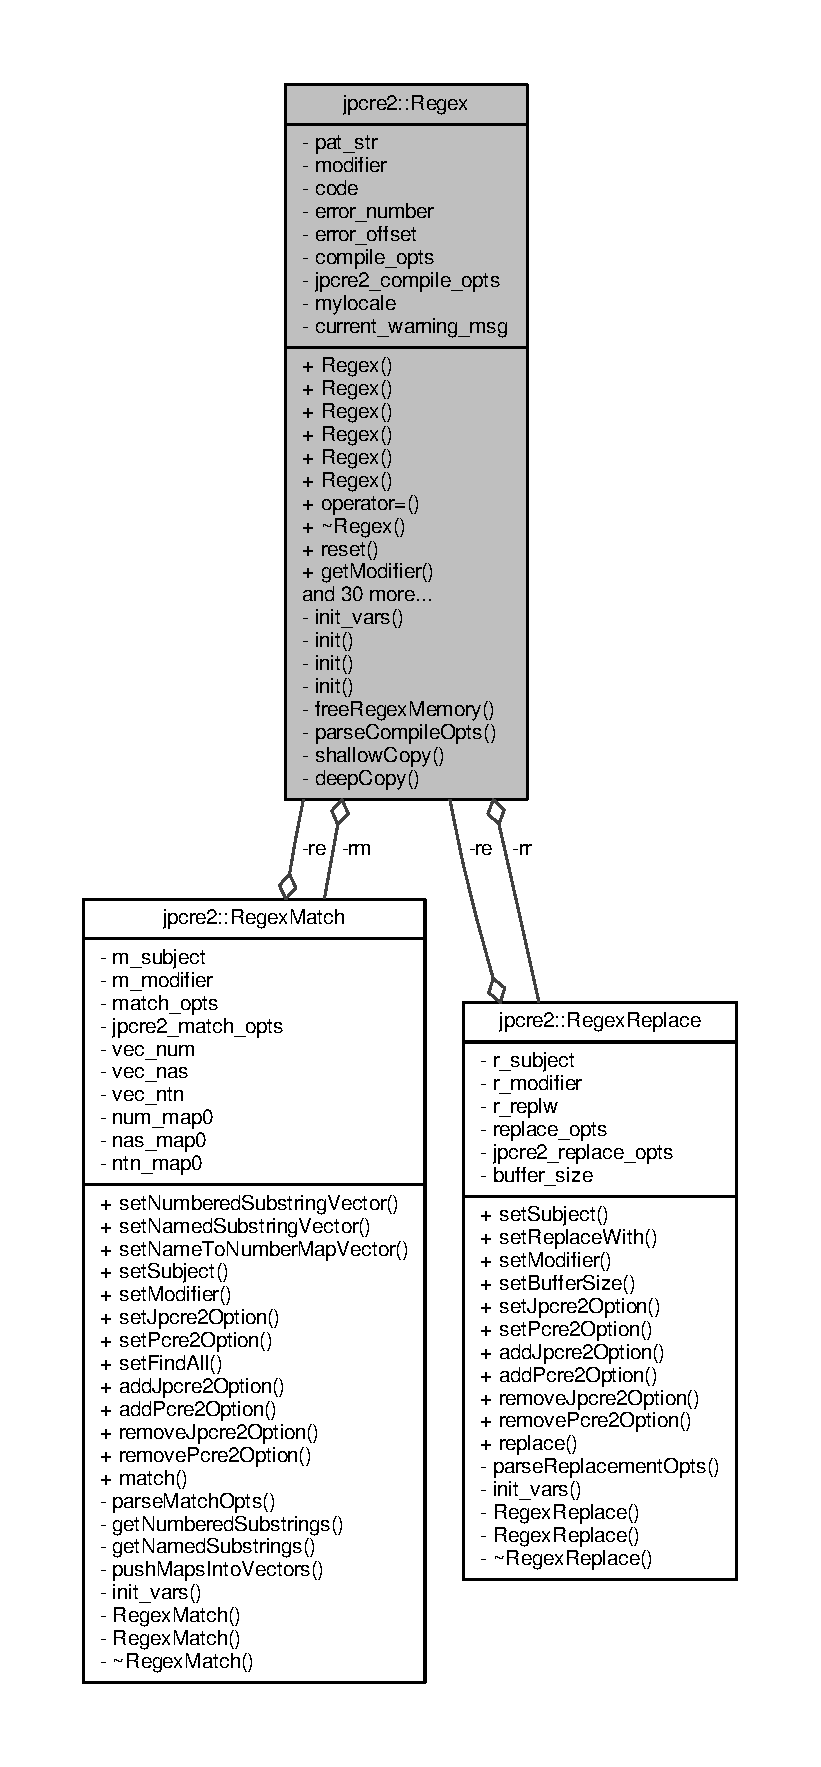
\includegraphics[height=550pt]{classjpcre2_1_1Regex__coll__graph}
\end{center}
\end{figure}
\subsubsection*{Public Member Functions}
\begin{DoxyCompactItemize}
\item 
\hyperlink{classjpcre2_1_1Regex_a302f65cd5747c5d34570ca76516ab715_a302f65cd5747c5d34570ca76516ab715}{Regex} ()
\begin{DoxyCompactList}\small\item\em Default Constructor. \end{DoxyCompactList}\item 
\hyperlink{classjpcre2_1_1Regex_a4d959fdc32791bee6d819abfc44af51a_a4d959fdc32791bee6d819abfc44af51a}{Regex} (const \hyperlink{namespacejpcre2_a91f03070152fb228bc116c5a737f1d16}{String} \&re)
\begin{DoxyCompactList}\small\item\em Compile pattern with initialization. \end{DoxyCompactList}\item 
\hyperlink{classjpcre2_1_1Regex_a58be9b4e1eaec2a43586af45c6ae5549_a58be9b4e1eaec2a43586af45c6ae5549}{Regex} (const \hyperlink{namespacejpcre2_a91f03070152fb228bc116c5a737f1d16}{String} \&re, const \hyperlink{namespacejpcre2_a91f03070152fb228bc116c5a737f1d16}{String} \&mod)
\begin{DoxyCompactList}\small\item\em This is an overloaded member function, provided for convenience. It differs from the above function only in what argument(s) it accepts. \end{DoxyCompactList}\item 
\hyperlink{classjpcre2_1_1Regex_a8f8a1eabf09292b782a6f33287e3fee4_a8f8a1eabf09292b782a6f33287e3fee4}{Regex} (const \hyperlink{namespacejpcre2_a91f03070152fb228bc116c5a737f1d16}{String} \&re, \hyperlink{namespacejpcre2_a078242d38221a13fb3543b9edd78c099}{Uint} pcre2\+\_\+opts)
\begin{DoxyCompactList}\small\item\em This is an overloaded member function, provided for convenience. It differs from the above function only in what argument(s) it accepts. \end{DoxyCompactList}\item 
\hyperlink{classjpcre2_1_1Regex_abe210e2ca6cfcef11760875930cf069d_abe210e2ca6cfcef11760875930cf069d}{Regex} (const \hyperlink{namespacejpcre2_a91f03070152fb228bc116c5a737f1d16}{String} \&re, \hyperlink{namespacejpcre2_a078242d38221a13fb3543b9edd78c099}{Uint} pcre2\+\_\+opts, \hyperlink{namespacejpcre2_a078242d38221a13fb3543b9edd78c099}{Uint} opt\+\_\+bits)
\begin{DoxyCompactList}\small\item\em This is an overloaded member function, provided for convenience. It differs from the above function only in what argument(s) it accepts. \end{DoxyCompactList}\item 
\hyperlink{classjpcre2_1_1Regex_ae03bb99a5bc8f945e693ddc34706f0c0_ae03bb99a5bc8f945e693ddc34706f0c0}{Regex} (const \hyperlink{classjpcre2_1_1Regex}{Regex} \&r)
\begin{DoxyCompactList}\small\item\em This is an overloaded member function, provided for convenience. It differs from the above function only in what argument(s) it accepts. Copy constructor. \end{DoxyCompactList}\item 
\hyperlink{classjpcre2_1_1Regex}{Regex} \& \hyperlink{classjpcre2_1_1Regex_ab43a14b4b6e75b7fa3221bc18a1d4121_ab43a14b4b6e75b7fa3221bc18a1d4121}{operator=} (const \hyperlink{classjpcre2_1_1Regex}{Regex} \&r)
\begin{DoxyCompactList}\small\item\em Overloaded assignment operator. \end{DoxyCompactList}\item 
\hyperlink{classjpcre2_1_1Regex_a9070a9f3adcaebccca5d15b247b93fda_a9070a9f3adcaebccca5d15b247b93fda}{operator bool} () const
\begin{DoxyCompactList}\small\item\em Provides boolean check for the status of the object. \end{DoxyCompactList}\item 
bool \hyperlink{classjpcre2_1_1Regex_afe102e21a96f5cfe12621746f899fa25_afe102e21a96f5cfe12621746f899fa25}{operator!} () const
\begin{DoxyCompactList}\small\item\em Provides boolean check for the status of the object. \end{DoxyCompactList}\item 
\hypertarget{classjpcre2_1_1Regex_a12b2bf254b59d7967681b77795c49260}{}\label{classjpcre2_1_1Regex_a12b2bf254b59d7967681b77795c49260} 
\hyperlink{classjpcre2_1_1Regex_a12b2bf254b59d7967681b77795c49260}{$\sim$\+Regex} ()
\begin{DoxyCompactList}\small\item\em Destructor Deletes memory used by \hyperlink{classjpcre2_1_1Regex_a447925705d222dbbd8c7d60b98cc65f0}{rm} an \hyperlink{classjpcre2_1_1Regex_a5a7ac6c6288988079b8933b4b6637fab}{rr}. \end{DoxyCompactList}\item 
\hyperlink{classjpcre2_1_1Regex}{Regex} \& \hyperlink{classjpcre2_1_1Regex_a91f6afe257e9633cbb79a98649ab8d02_a91f6afe257e9633cbb79a98649ab8d02}{reset} ()
\begin{DoxyCompactList}\small\item\em Reset all class variables to its default (initial) state. \end{DoxyCompactList}\item 
\hyperlink{classjpcre2_1_1Regex}{Regex} \& \hyperlink{classjpcre2_1_1Regex_aff12a6e75ecd3e623875d12df49b3b89_aff12a6e75ecd3e623875d12df49b3b89}{reset\+Errors} ()
\begin{DoxyCompactList}\small\item\em Reset errors to zero. \end{DoxyCompactList}\item 
\hyperlink{namespacejpcre2_a91f03070152fb228bc116c5a737f1d16}{String} \hyperlink{classjpcre2_1_1Regex_a006dd17f71a2d717aa9575d72fac6d7b_a006dd17f71a2d717aa9575d72fac6d7b}{get\+Pattern} ()
\begin{DoxyCompactList}\small\item\em Get pattern string. \end{DoxyCompactList}\item 
\hyperlink{namespacejpcre2_a91f03070152fb228bc116c5a737f1d16}{String} \hyperlink{classjpcre2_1_1Regex_ae9afaf627ed922a9e4cee8074d30edfa_ae9afaf627ed922a9e4cee8074d30edfa}{get\+Locale} ()
\begin{DoxyCompactList}\small\item\em Get locale as a string. \end{DoxyCompactList}\item 
\hyperlink{namespacejpcre2_a91f03070152fb228bc116c5a737f1d16}{String} \hyperlink{classjpcre2_1_1Regex_a0ac4e063f00128b96cd94c33609dc559_a0ac4e063f00128b96cd94c33609dc559}{get\+Modifier} ()
\begin{DoxyCompactList}\small\item\em Get modifier string calculated from J\+P\+C\+R\+E2 and P\+C\+R\+E2 options. \end{DoxyCompactList}\item 
\hyperlink{namespacejpcre2_a078242d38221a13fb3543b9edd78c099}{Uint} \hyperlink{classjpcre2_1_1Regex_a857307fc59ba7f010b097e61c1744923_a857307fc59ba7f010b097e61c1744923}{get\+Pcre2\+Option} ()
\begin{DoxyCompactList}\small\item\em Get P\+C\+R\+E2 option. \end{DoxyCompactList}\item 
\hyperlink{namespacejpcre2_a078242d38221a13fb3543b9edd78c099}{Uint} \hyperlink{classjpcre2_1_1Regex_a5d2d04eb7c393338a4c8cce941e957ef_a5d2d04eb7c393338a4c8cce941e957ef}{get\+Jpcre2\+Option} ()
\begin{DoxyCompactList}\small\item\em Get J\+P\+C\+R\+E2 option. \end{DoxyCompactList}\item 
int \hyperlink{classjpcre2_1_1Regex_a7294273e7d11907a749f2db40da9ed15_a7294273e7d11907a749f2db40da9ed15}{get\+Error\+Number} ()
\begin{DoxyCompactList}\small\item\em Returns the last error number. \end{DoxyCompactList}\item 
int \hyperlink{classjpcre2_1_1Regex_ae8c6c8f728c58d9b171c68b4b166e195_ae8c6c8f728c58d9b171c68b4b166e195}{get\+Error\+Offset} ()
\begin{DoxyCompactList}\small\item\em Returns the last error offset. \end{DoxyCompactList}\item 
int \hyperlink{classjpcre2_1_1Regex_a6aa5722e52a154a1594ee6ea46e5d888_a6aa5722e52a154a1594ee6ea46e5d888}{get\+Warning\+Number} ()
\begin{DoxyCompactList}\small\item\em Returns the last warning number. \end{DoxyCompactList}\item 
int \hyperlink{classjpcre2_1_1Regex_a18dddb3eeedf5c61e0169770ffc9ab8f_a18dddb3eeedf5c61e0169770ffc9ab8f}{get\+Warningoffset} ()
\begin{DoxyCompactList}\small\item\em Returns the last warning offset. \end{DoxyCompactList}\item 
\hyperlink{namespacejpcre2_a91f03070152fb228bc116c5a737f1d16}{String} \hyperlink{classjpcre2_1_1Regex_a8606fff8b192c94f58ca9e82aa048c61_a8606fff8b192c94f58ca9e82aa048c61}{get\+Error\+Message} ()
\begin{DoxyCompactList}\small\item\em Returns the last error message. \end{DoxyCompactList}\item 
\hyperlink{namespacejpcre2_a91f03070152fb228bc116c5a737f1d16}{String} \hyperlink{classjpcre2_1_1Regex_a1a639ae4090b88609c03e9268faf02d8_a1a639ae4090b88609c03e9268faf02d8}{get\+Warning\+Message} ()
\begin{DoxyCompactList}\small\item\em Returns the last warning message. \end{DoxyCompactList}\item 
\hyperlink{classjpcre2_1_1Regex}{Regex} \& \hyperlink{classjpcre2_1_1Regex_a85d9a514ea86ae68533223adac6c6bd8_a85d9a514ea86ae68533223adac6c6bd8}{set\+Pattern} (const \hyperlink{namespacejpcre2_a91f03070152fb228bc116c5a737f1d16}{String} \&re)
\begin{DoxyCompactList}\small\item\em Set the Pattern string \hyperlink{classjpcre2_1_1Regex_a0bceb85b6dbba355b56b5cc312214435}{pat\+\_\+str}. \end{DoxyCompactList}\item 
\hyperlink{classjpcre2_1_1Regex}{Regex} \& \hyperlink{classjpcre2_1_1Regex_aed9865b58c60945e19f36fa310f5a595_aed9865b58c60945e19f36fa310f5a595}{set\+Modifier} (const \hyperlink{namespacejpcre2_a91f03070152fb228bc116c5a737f1d16}{String} \&x)
\begin{DoxyCompactList}\small\item\em Set the modifier (overwrite existing J\+P\+C\+R\+E2 and P\+C\+R\+E2 option). \end{DoxyCompactList}\item 
\hyperlink{classjpcre2_1_1Regex}{Regex} \& \hyperlink{classjpcre2_1_1Regex_a56721534519e5cb436337043eee8f42d_a56721534519e5cb436337043eee8f42d}{set\+Locale} (const \hyperlink{namespacejpcre2_a91f03070152fb228bc116c5a737f1d16}{String} \&x)
\begin{DoxyCompactList}\small\item\em Set the locale \hyperlink{classjpcre2_1_1Regex_a92a3ad992cade62d103248302f7e2f2d}{mylocale}. \end{DoxyCompactList}\item 
\hyperlink{classjpcre2_1_1Regex}{Regex} \& \hyperlink{classjpcre2_1_1Regex_a031617a19638ef752dcd2b29fa3464d5_a031617a19638ef752dcd2b29fa3464d5}{set\+Jpcre2\+Option} (\hyperlink{namespacejpcre2_a078242d38221a13fb3543b9edd78c099}{Uint} x)
\begin{DoxyCompactList}\small\item\em Set J\+P\+C\+R\+E2 option \hyperlink{classjpcre2_1_1Regex_abdd26c3bc1c3132f0aa73dde1690a7ef}{jpcre2\+\_\+compile\+\_\+opts} (overwrites existing option) \end{DoxyCompactList}\item 
\hyperlink{classjpcre2_1_1Regex}{Regex} \& \hyperlink{classjpcre2_1_1Regex_acdc6f97f4030ae109c4e1a4e2310bceb_acdc6f97f4030ae109c4e1a4e2310bceb}{set\+Pcre2\+Option} (\hyperlink{namespacejpcre2_a078242d38221a13fb3543b9edd78c099}{Uint} x)
\begin{DoxyCompactList}\small\item\em Set P\+C\+R\+E2 option \hyperlink{classjpcre2_1_1Regex_a5954131e9085de63229ed5c11417df69}{compile\+\_\+opts} (overwrites existing option) \end{DoxyCompactList}\item 
\hyperlink{classjpcre2_1_1Regex}{Regex} \& \hyperlink{classjpcre2_1_1Regex_a9ab3efed9819a51225456e6d8487de56_a9ab3efed9819a51225456e6d8487de56}{change\+Modifier} (const \hyperlink{namespacejpcre2_a91f03070152fb228bc116c5a737f1d16}{String} \&, bool)
\begin{DoxyCompactList}\small\item\em Parse modifier and add/remove equivalent P\+C\+R\+E2 and J\+P\+C\+R\+E2 options. \end{DoxyCompactList}\item 
\hyperlink{classjpcre2_1_1Regex}{Regex} \& \hyperlink{classjpcre2_1_1Regex_ab8e0b1a49eeb1077ba54cf3b5292c95e_ab8e0b1a49eeb1077ba54cf3b5292c95e}{change\+Jpcre2\+Option} (\hyperlink{namespacejpcre2_a078242d38221a13fb3543b9edd78c099}{Uint} opt, bool x)
\begin{DoxyCompactList}\small\item\em Add or remove a J\+P\+C\+R\+E2 option. \end{DoxyCompactList}\item 
\hyperlink{classjpcre2_1_1Regex}{Regex} \& \hyperlink{classjpcre2_1_1Regex_ae5bde8008cc5a700163ca3162dbd5823_ae5bde8008cc5a700163ca3162dbd5823}{change\+Pcre2\+Option} (\hyperlink{namespacejpcre2_a078242d38221a13fb3543b9edd78c099}{Uint} opt, bool x)
\begin{DoxyCompactList}\small\item\em Add or remove a P\+C\+R\+E2 option. \end{DoxyCompactList}\item 
\hyperlink{classjpcre2_1_1Regex}{Regex} \& \hyperlink{classjpcre2_1_1Regex_ab1af1471339602446d8221b8c97c6b55_ab1af1471339602446d8221b8c97c6b55}{add\+Modifier} (const \hyperlink{namespacejpcre2_a91f03070152fb228bc116c5a737f1d16}{String} \&mod)
\begin{DoxyCompactList}\small\item\em Parse modifier string and add equivalent P\+C\+R\+E2 and J\+P\+C\+R\+E2 options. \end{DoxyCompactList}\item 
\hyperlink{classjpcre2_1_1Regex}{Regex} \& \hyperlink{classjpcre2_1_1Regex_a03974fa7ba8f7c47186cb8d6f54934de_a03974fa7ba8f7c47186cb8d6f54934de}{add\+Jpcre2\+Option} (\hyperlink{namespacejpcre2_a078242d38221a13fb3543b9edd78c099}{Uint} x)
\begin{DoxyCompactList}\small\item\em Add option to existing J\+P\+C\+R\+E2 options \hyperlink{classjpcre2_1_1Regex_abdd26c3bc1c3132f0aa73dde1690a7ef}{jpcre2\+\_\+compile\+\_\+opts}. \end{DoxyCompactList}\item 
\hyperlink{classjpcre2_1_1Regex}{Regex} \& \hyperlink{classjpcre2_1_1Regex_a2c7dcf12f26b2b046e147b013c8b5087_a2c7dcf12f26b2b046e147b013c8b5087}{add\+Pcre2\+Option} (\hyperlink{namespacejpcre2_a078242d38221a13fb3543b9edd78c099}{Uint} x)
\begin{DoxyCompactList}\small\item\em Add option to existing P\+C\+R\+E2 options \hyperlink{classjpcre2_1_1Regex_a5954131e9085de63229ed5c11417df69}{compile\+\_\+opts}. \end{DoxyCompactList}\item 
void \hyperlink{classjpcre2_1_1Regex_aad1d5ef1e87f762f68a587eec4022e69_aad1d5ef1e87f762f68a587eec4022e69}{compile} (void)
\begin{DoxyCompactList}\small\item\em Compile the regex pattern from class variable \hyperlink{classjpcre2_1_1Regex_a0bceb85b6dbba355b56b5cc312214435}{pat\+\_\+str}. \end{DoxyCompactList}\item 
void \hyperlink{classjpcre2_1_1Regex_a4640915bc907aa3b80da543f1eb7e74f_a4640915bc907aa3b80da543f1eb7e74f}{compile} (const \hyperlink{namespacejpcre2_a91f03070152fb228bc116c5a737f1d16}{String} \&re, \hyperlink{namespacejpcre2_a078242d38221a13fb3543b9edd78c099}{Uint} po, \hyperlink{namespacejpcre2_a078242d38221a13fb3543b9edd78c099}{Uint} jo)
\begin{DoxyCompactList}\small\item\em This is an overloaded member function, provided for convenience. It differs from the above function only in what argument(s) it accepts. \end{DoxyCompactList}\item 
void \hyperlink{classjpcre2_1_1Regex_a01394dcb222c4d442cabbffb4bcf570a_a01394dcb222c4d442cabbffb4bcf570a}{compile} (const \hyperlink{namespacejpcre2_a91f03070152fb228bc116c5a737f1d16}{String} \&re, \hyperlink{namespacejpcre2_a078242d38221a13fb3543b9edd78c099}{Uint} po)
\begin{DoxyCompactList}\small\item\em This is an overloaded member function, provided for convenience. It differs from the above function only in what argument(s) it accepts. \end{DoxyCompactList}\item 
void \hyperlink{classjpcre2_1_1Regex_acd49e856009160c622e90b81b6557d8d_acd49e856009160c622e90b81b6557d8d}{compile} (const \hyperlink{namespacejpcre2_a91f03070152fb228bc116c5a737f1d16}{String} \&re, const \hyperlink{namespacejpcre2_a91f03070152fb228bc116c5a737f1d16}{String} \&mod)
\begin{DoxyCompactList}\small\item\em This is an overloaded member function, provided for convenience. It differs from the above function only in what argument(s) it accepts. \end{DoxyCompactList}\item 
void \hyperlink{classjpcre2_1_1Regex_a81687ca434654cae776c2854c3618de0_a81687ca434654cae776c2854c3618de0}{compile} (const \hyperlink{namespacejpcre2_a91f03070152fb228bc116c5a737f1d16}{String} \&re)
\begin{DoxyCompactList}\small\item\em This is an overloaded member function, provided for convenience. It differs from the above function only in what argument(s) it accepts. \end{DoxyCompactList}\item 
\hyperlink{namespacejpcre2_a2aac465ddcb123560c7c8215dd69246c}{S\+I\+Z\+E\+\_\+T} \hyperlink{classjpcre2_1_1Regex_ab93775a93a0a537d09b9e9ab4a5a3894_ab93775a93a0a537d09b9e9ab4a5a3894}{match} (const \hyperlink{namespacejpcre2_a91f03070152fb228bc116c5a737f1d16}{String} \&s, const \hyperlink{namespacejpcre2_a91f03070152fb228bc116c5a737f1d16}{String} \&mod)
\begin{DoxyCompactList}\small\item\em Perform regex match and return match count. \end{DoxyCompactList}\item 
\hyperlink{namespacejpcre2_a2aac465ddcb123560c7c8215dd69246c}{S\+I\+Z\+E\+\_\+T} \hyperlink{classjpcre2_1_1Regex_a9ffbb6aa54cb97125f1b4211bc1d09a5_a9ffbb6aa54cb97125f1b4211bc1d09a5}{match} (const \hyperlink{namespacejpcre2_a91f03070152fb228bc116c5a737f1d16}{String} \&s)
\begin{DoxyCompactList}\small\item\em This is an overloaded member function, provided for convenience. It differs from the above function only in what argument(s) it accepts. \end{DoxyCompactList}\item 
\hyperlink{classjpcre2_1_1RegexMatch}{Regex\+Match} \& \hyperlink{classjpcre2_1_1Regex_a519b0915bf1163c6ce6a4d674b30cfcd_a519b0915bf1163c6ce6a4d674b30cfcd}{init\+Match} ()
\begin{DoxyCompactList}\small\item\em Prepare to call \hyperlink{classjpcre2_1_1RegexMatch_a5868aef3a146594ea1ebef34d122bb33_a5868aef3a146594ea1ebef34d122bb33}{Regex\+Match\+::match()}. \end{DoxyCompactList}\item 
\hyperlink{classjpcre2_1_1RegexMatch}{Regex\+Match} \& \hyperlink{classjpcre2_1_1Regex_abb007e99d7e2188ec80b741e7b40668f_abb007e99d7e2188ec80b741e7b40668f}{get\+Match\+Object} ()
\begin{DoxyCompactList}\small\item\em returns a reference to existing match object. \end{DoxyCompactList}\item 
\hyperlink{namespacejpcre2_a91f03070152fb228bc116c5a737f1d16}{String} \hyperlink{classjpcre2_1_1Regex_ac592ce7a5e4210ed5f90a0105b1f2981_ac592ce7a5e4210ed5f90a0105b1f2981}{replace} (const \hyperlink{namespacejpcre2_a91f03070152fb228bc116c5a737f1d16}{String} \&mains, const \hyperlink{namespacejpcre2_a91f03070152fb228bc116c5a737f1d16}{String} \&repl, const \hyperlink{namespacejpcre2_a91f03070152fb228bc116c5a737f1d16}{String} \&mod)
\begin{DoxyCompactList}\small\item\em Perform regex replace and return the replaced string. \end{DoxyCompactList}\item 
\hyperlink{namespacejpcre2_a91f03070152fb228bc116c5a737f1d16}{String} \hyperlink{classjpcre2_1_1Regex_addd7c21abd0f4cf6c532a7602cfb5835_addd7c21abd0f4cf6c532a7602cfb5835}{replace} (const \hyperlink{namespacejpcre2_a91f03070152fb228bc116c5a737f1d16}{String} \&mains, const \hyperlink{namespacejpcre2_a91f03070152fb228bc116c5a737f1d16}{String} \&repl)
\begin{DoxyCompactList}\small\item\em This is an overloaded member function, provided for convenience. It differs from the above function only in what argument(s) it accepts. \end{DoxyCompactList}\item 
\hyperlink{classjpcre2_1_1RegexReplace}{Regex\+Replace} \& \hyperlink{classjpcre2_1_1Regex_ae7235a991492fa88f1bd3fb02d59cd0a_ae7235a991492fa88f1bd3fb02d59cd0a}{init\+Replace} ()
\begin{DoxyCompactList}\small\item\em Prepare to call \hyperlink{classjpcre2_1_1RegexReplace_afd087fa7a9bfedec802d1a3dd7edbdd0_afd087fa7a9bfedec802d1a3dd7edbdd0}{Regex\+Replace\+::replace()}. \end{DoxyCompactList}\item 
\hyperlink{classjpcre2_1_1RegexReplace}{Regex\+Replace} \& \hyperlink{classjpcre2_1_1Regex_ad0b5e492eae75ef13b3d80f4fb1e3486_ad0b5e492eae75ef13b3d80f4fb1e3486}{get\+Replace\+Object} ()
\begin{DoxyCompactList}\small\item\em returns a reference to the existing \hyperlink{classjpcre2_1_1RegexReplace}{Regex\+Replace} object. \end{DoxyCompactList}\end{DoxyCompactItemize}
\subsubsection*{Private Member Functions}
\begin{DoxyCompactItemize}
\item 
\hypertarget{classjpcre2_1_1Regex_aff1f5cd95b6ac227014e7a5265a50cc0}{}\label{classjpcre2_1_1Regex_aff1f5cd95b6ac227014e7a5265a50cc0} 
void \hyperlink{classjpcre2_1_1Regex_aff1f5cd95b6ac227014e7a5265a50cc0}{init\+\_\+vars} ()
\begin{DoxyCompactList}\small\item\em Initialize class variables. \end{DoxyCompactList}\item 
void \hyperlink{classjpcre2_1_1Regex_a6df564d3dec70bbeec65de125c7d4de2_a6df564d3dec70bbeec65de125c7d4de2}{init} ()
\begin{DoxyCompactList}\small\item\em Call \hyperlink{classjpcre2_1_1Regex_aff1f5cd95b6ac227014e7a5265a50cc0}{Regex\+::init\+\_\+vars()} and initialize class variables. \end{DoxyCompactList}\item 
void \hyperlink{classjpcre2_1_1Regex_aedc5f414e5fa401e1a91614cfab0b033_aedc5f414e5fa401e1a91614cfab0b033}{init} (const \hyperlink{namespacejpcre2_a91f03070152fb228bc116c5a737f1d16}{String} \&re, const \hyperlink{namespacejpcre2_a91f03070152fb228bc116c5a737f1d16}{String} \&mod)
\begin{DoxyCompactList}\small\item\em This is an overloaded member function, provided for convenience. It differs from the above function only in what argument(s) it accepts. \end{DoxyCompactList}\item 
void \hyperlink{classjpcre2_1_1Regex_adbda074677e393438452190e55a971d0_adbda074677e393438452190e55a971d0}{init} (const \hyperlink{namespacejpcre2_a91f03070152fb228bc116c5a737f1d16}{String} \&re, \hyperlink{namespacejpcre2_a078242d38221a13fb3543b9edd78c099}{Uint} po, \hyperlink{namespacejpcre2_a078242d38221a13fb3543b9edd78c099}{Uint} jo)
\begin{DoxyCompactList}\small\item\em This is an overloaded member function, provided for convenience. It differs from the above function only in what argument(s) it accepts. \end{DoxyCompactList}\item 
\hypertarget{classjpcre2_1_1Regex_a40128e1facd915e06089eeb17e2287c2}{}\label{classjpcre2_1_1Regex_a40128e1facd915e06089eeb17e2287c2} 
void \hyperlink{classjpcre2_1_1Regex_a40128e1facd915e06089eeb17e2287c2}{free\+Regex\+Memory} (void)
\begin{DoxyCompactList}\small\item\em Free \hyperlink{classjpcre2_1_1Regex_a2742264206d8976c413b474b7bac4b2e}{code} if it\textquotesingle{}s non-\/\+N\+U\+LL. \end{DoxyCompactList}\item 
\hypertarget{classjpcre2_1_1Regex_a24594d3bdb08b3795080c68019928f3a}{}\label{classjpcre2_1_1Regex_a24594d3bdb08b3795080c68019928f3a} 
void \hyperlink{classjpcre2_1_1Regex_a24594d3bdb08b3795080c68019928f3a}{shallow\+Copy} (const \hyperlink{classjpcre2_1_1Regex}{Regex} \&r)
\begin{DoxyCompactList}\small\item\em Do a shallow copy of class variables. \end{DoxyCompactList}\item 
void \hyperlink{classjpcre2_1_1Regex_a240790a0f3d8e97af0a76ad3f882e02a_a240790a0f3d8e97af0a76ad3f882e02a}{deep\+Copy} (const \hyperlink{classjpcre2_1_1Regex}{Regex} \&)
\begin{DoxyCompactList}\small\item\em Do a deep copy of \hyperlink{classjpcre2_1_1Regex_a447925705d222dbbd8c7d60b98cc65f0}{rm}, \hyperlink{classjpcre2_1_1Regex_a5a7ac6c6288988079b8933b4b6637fab}{rr} and \hyperlink{classjpcre2_1_1Regex_a2742264206d8976c413b474b7bac4b2e}{code}. \end{DoxyCompactList}\end{DoxyCompactItemize}
\subsubsection*{Private Attributes}
\begin{DoxyCompactItemize}
\item 
\hypertarget{classjpcre2_1_1Regex_a447925705d222dbbd8c7d60b98cc65f0}{}\label{classjpcre2_1_1Regex_a447925705d222dbbd8c7d60b98cc65f0} 
\hyperlink{classjpcre2_1_1RegexMatch}{Regex\+Match} $\ast$ \hyperlink{classjpcre2_1_1Regex_a447925705d222dbbd8c7d60b98cc65f0}{rm}
\begin{DoxyCompactList}\small\item\em Pointer to \hyperlink{classjpcre2_1_1RegexMatch}{Regex\+Match} object. \end{DoxyCompactList}\item 
\hypertarget{classjpcre2_1_1Regex_a5a7ac6c6288988079b8933b4b6637fab}{}\label{classjpcre2_1_1Regex_a5a7ac6c6288988079b8933b4b6637fab} 
\hyperlink{classjpcre2_1_1RegexReplace}{Regex\+Replace} $\ast$ \hyperlink{classjpcre2_1_1Regex_a5a7ac6c6288988079b8933b4b6637fab}{rr}
\begin{DoxyCompactList}\small\item\em Pointer to \hyperlink{classjpcre2_1_1RegexReplace}{Regex\+Replace} object. \end{DoxyCompactList}\item 
\hypertarget{classjpcre2_1_1Regex_a0bceb85b6dbba355b56b5cc312214435}{}\label{classjpcre2_1_1Regex_a0bceb85b6dbba355b56b5cc312214435} 
\hyperlink{namespacejpcre2_a91f03070152fb228bc116c5a737f1d16}{String} \hyperlink{classjpcre2_1_1Regex_a0bceb85b6dbba355b56b5cc312214435}{pat\+\_\+str}
\begin{DoxyCompactList}\small\item\em Pattern string. \end{DoxyCompactList}\item 
\hypertarget{classjpcre2_1_1Regex_a2742264206d8976c413b474b7bac4b2e}{}\label{classjpcre2_1_1Regex_a2742264206d8976c413b474b7bac4b2e} 
pcre2\+\_\+code $\ast$ \hyperlink{classjpcre2_1_1Regex_a2742264206d8976c413b474b7bac4b2e}{code}
\begin{DoxyCompactList}\small\item\em Pointer to compiled pattern. \end{DoxyCompactList}\item 
\hypertarget{classjpcre2_1_1Regex_a5954131e9085de63229ed5c11417df69}{}\label{classjpcre2_1_1Regex_a5954131e9085de63229ed5c11417df69} 
\hyperlink{namespacejpcre2_a078242d38221a13fb3543b9edd78c099}{Uint} \hyperlink{classjpcre2_1_1Regex_a5954131e9085de63229ed5c11417df69}{compile\+\_\+opts}
\begin{DoxyCompactList}\small\item\em Compile options for P\+C\+R\+E2 (used by P\+C\+R\+E2 internal function pcre2\+\_\+compile()) \end{DoxyCompactList}\item 
\hypertarget{classjpcre2_1_1Regex_abdd26c3bc1c3132f0aa73dde1690a7ef}{}\label{classjpcre2_1_1Regex_abdd26c3bc1c3132f0aa73dde1690a7ef} 
\hyperlink{namespacejpcre2_a078242d38221a13fb3543b9edd78c099}{Uint} \hyperlink{classjpcre2_1_1Regex_abdd26c3bc1c3132f0aa73dde1690a7ef}{jpcre2\+\_\+compile\+\_\+opts}
\begin{DoxyCompactList}\small\item\em Compile options specific to J\+P\+C\+R\+E2. \end{DoxyCompactList}\item 
\hypertarget{classjpcre2_1_1Regex_a92a3ad992cade62d103248302f7e2f2d}{}\label{classjpcre2_1_1Regex_a92a3ad992cade62d103248302f7e2f2d} 
\hyperlink{namespacejpcre2_a91f03070152fb228bc116c5a737f1d16}{String} \hyperlink{classjpcre2_1_1Regex_a92a3ad992cade62d103248302f7e2f2d}{mylocale}
\begin{DoxyCompactList}\small\item\em Locale as a string. \end{DoxyCompactList}\item 
\hypertarget{classjpcre2_1_1Regex_a91b7b795c9efe76ef4e015325ff33f1c}{}\label{classjpcre2_1_1Regex_a91b7b795c9efe76ef4e015325ff33f1c} 
int \hyperlink{classjpcre2_1_1Regex_a91b7b795c9efe76ef4e015325ff33f1c}{error\+\_\+number}
\begin{DoxyCompactList}\small\item\em Last error number. \end{DoxyCompactList}\item 
\hypertarget{classjpcre2_1_1Regex_a0b9613704582b9c6b0175a21a2a421e0}{}\label{classjpcre2_1_1Regex_a0b9613704582b9c6b0175a21a2a421e0} 
P\+C\+R\+E2\+\_\+\+S\+I\+ZE \hyperlink{classjpcre2_1_1Regex_a0b9613704582b9c6b0175a21a2a421e0}{error\+\_\+offset}
\begin{DoxyCompactList}\small\item\em Last error offset. \end{DoxyCompactList}\item 
\hypertarget{classjpcre2_1_1Regex_a24f70c6c8e7984b3f8c5ae9eb2d2c5ae}{}\label{classjpcre2_1_1Regex_a24f70c6c8e7984b3f8c5ae9eb2d2c5ae} 
int \hyperlink{classjpcre2_1_1Regex_a24f70c6c8e7984b3f8c5ae9eb2d2c5ae}{warning\+\_\+number}
\begin{DoxyCompactList}\small\item\em Last warning number. \end{DoxyCompactList}\item 
\hypertarget{classjpcre2_1_1Regex_ad19f84b5120ddcfc0776c0a8e8aa5351}{}\label{classjpcre2_1_1Regex_ad19f84b5120ddcfc0776c0a8e8aa5351} 
int \hyperlink{classjpcre2_1_1Regex_ad19f84b5120ddcfc0776c0a8e8aa5351}{warning\+\_\+offset}
\begin{DoxyCompactList}\small\item\em Last warning offset. \end{DoxyCompactList}\end{DoxyCompactItemize}
\subsubsection*{Friends}
\begin{DoxyCompactItemize}
\item 
\hypertarget{classjpcre2_1_1Regex_aaa8d9b93cf5a8b9ebbb78923a1494445}{}\label{classjpcre2_1_1Regex_aaa8d9b93cf5a8b9ebbb78923a1494445} 
class \hyperlink{classjpcre2_1_1Regex_aaa8d9b93cf5a8b9ebbb78923a1494445}{Regex\+Match}
\begin{DoxyCompactList}\small\item\em Define \hyperlink{classjpcre2_1_1RegexMatch}{Regex\+Match} as friends. It needs to access the compiled pattern which is a private property of this class. \end{DoxyCompactList}\item 
\hypertarget{classjpcre2_1_1Regex_a2547cb5380cbe0374ac0d44d34018dbb}{}\label{classjpcre2_1_1Regex_a2547cb5380cbe0374ac0d44d34018dbb} 
class \hyperlink{classjpcre2_1_1Regex_a2547cb5380cbe0374ac0d44d34018dbb}{Regex\+Replace}
\begin{DoxyCompactList}\small\item\em Define \hyperlink{classjpcre2_1_1RegexReplace}{Regex\+Replace} as friends. It needs to access the compiled pattern which is a private property of this class. \end{DoxyCompactList}\end{DoxyCompactItemize}


\subsubsection{Detailed Description}
Implements public overloaded and copy constructors, provides functions to set/unset various options and perform regex match and replace against a compiled pattern. 

Each regex pattern needs an object of this class.

A pattern must be compiled either by explicitly calling the compile function or using one of the parameterized constructors. 

\subsubsection{Constructor \& Destructor Documentation}
\hypertarget{classjpcre2_1_1Regex_a302f65cd5747c5d34570ca76516ab715_a302f65cd5747c5d34570ca76516ab715}{}\label{classjpcre2_1_1Regex_a302f65cd5747c5d34570ca76516ab715_a302f65cd5747c5d34570ca76516ab715} 
\index{jpcre2\+::\+Regex@{jpcre2\+::\+Regex}!Regex@{Regex}}
\index{Regex@{Regex}!jpcre2\+::\+Regex@{jpcre2\+::\+Regex}}
\paragraph{\texorpdfstring{Regex()}{Regex()}\hspace{0.1cm}{\footnotesize\ttfamily [1/6]}}
{\footnotesize\ttfamily jpcre2\+::\+Regex\+::\+Regex (\begin{DoxyParamCaption}{ }\end{DoxyParamCaption})\hspace{0.3cm}{\ttfamily [inline]}}



Default Constructor. 

Initializes all class variables to defaults. Does not perform any compilation. \hypertarget{classjpcre2_1_1Regex_a4d959fdc32791bee6d819abfc44af51a_a4d959fdc32791bee6d819abfc44af51a}{}\label{classjpcre2_1_1Regex_a4d959fdc32791bee6d819abfc44af51a_a4d959fdc32791bee6d819abfc44af51a} 
\index{jpcre2\+::\+Regex@{jpcre2\+::\+Regex}!Regex@{Regex}}
\index{Regex@{Regex}!jpcre2\+::\+Regex@{jpcre2\+::\+Regex}}
\paragraph{\texorpdfstring{Regex()}{Regex()}\hspace{0.1cm}{\footnotesize\ttfamily [2/6]}}
{\footnotesize\ttfamily jpcre2\+::\+Regex\+::\+Regex (\begin{DoxyParamCaption}\item[{const \hyperlink{namespacejpcre2_a91f03070152fb228bc116c5a737f1d16}{String} \&}]{re }\end{DoxyParamCaption})\hspace{0.3cm}{\ttfamily [inline]}}



Compile pattern with initialization. 


\begin{DoxyParams}{Parameters}
{\em re} & Pattern string \\
\hline
\end{DoxyParams}
\hypertarget{classjpcre2_1_1Regex_a58be9b4e1eaec2a43586af45c6ae5549_a58be9b4e1eaec2a43586af45c6ae5549}{}\label{classjpcre2_1_1Regex_a58be9b4e1eaec2a43586af45c6ae5549_a58be9b4e1eaec2a43586af45c6ae5549} 
\index{jpcre2\+::\+Regex@{jpcre2\+::\+Regex}!Regex@{Regex}}
\index{Regex@{Regex}!jpcre2\+::\+Regex@{jpcre2\+::\+Regex}}
\paragraph{\texorpdfstring{Regex()}{Regex()}\hspace{0.1cm}{\footnotesize\ttfamily [3/6]}}
{\footnotesize\ttfamily jpcre2\+::\+Regex\+::\+Regex (\begin{DoxyParamCaption}\item[{const \hyperlink{namespacejpcre2_a91f03070152fb228bc116c5a737f1d16}{String} \&}]{re,  }\item[{const \hyperlink{namespacejpcre2_a91f03070152fb228bc116c5a737f1d16}{String} \&}]{mod }\end{DoxyParamCaption})\hspace{0.3cm}{\ttfamily [inline]}}



This is an overloaded member function, provided for convenience. It differs from the above function only in what argument(s) it accepts. 

Compile pattern. 
\begin{DoxyParams}{Parameters}
{\em re} & Pattern string \\
\hline
{\em mod} & Modifier string \\
\hline
\end{DoxyParams}
\hypertarget{classjpcre2_1_1Regex_a8f8a1eabf09292b782a6f33287e3fee4_a8f8a1eabf09292b782a6f33287e3fee4}{}\label{classjpcre2_1_1Regex_a8f8a1eabf09292b782a6f33287e3fee4_a8f8a1eabf09292b782a6f33287e3fee4} 
\index{jpcre2\+::\+Regex@{jpcre2\+::\+Regex}!Regex@{Regex}}
\index{Regex@{Regex}!jpcre2\+::\+Regex@{jpcre2\+::\+Regex}}
\paragraph{\texorpdfstring{Regex()}{Regex()}\hspace{0.1cm}{\footnotesize\ttfamily [4/6]}}
{\footnotesize\ttfamily jpcre2\+::\+Regex\+::\+Regex (\begin{DoxyParamCaption}\item[{const \hyperlink{namespacejpcre2_a91f03070152fb228bc116c5a737f1d16}{String} \&}]{re,  }\item[{\hyperlink{namespacejpcre2_a078242d38221a13fb3543b9edd78c099}{Uint}}]{pcre2\+\_\+opts }\end{DoxyParamCaption})\hspace{0.3cm}{\ttfamily [inline]}}



This is an overloaded member function, provided for convenience. It differs from the above function only in what argument(s) it accepts. 

Compile pattern. 
\begin{DoxyParams}{Parameters}
{\em re} & Pattern string \\
\hline
{\em pcre2\+\_\+opts} & P\+C\+R\+E2 option value \\
\hline
\end{DoxyParams}
\hypertarget{classjpcre2_1_1Regex_abe210e2ca6cfcef11760875930cf069d_abe210e2ca6cfcef11760875930cf069d}{}\label{classjpcre2_1_1Regex_abe210e2ca6cfcef11760875930cf069d_abe210e2ca6cfcef11760875930cf069d} 
\index{jpcre2\+::\+Regex@{jpcre2\+::\+Regex}!Regex@{Regex}}
\index{Regex@{Regex}!jpcre2\+::\+Regex@{jpcre2\+::\+Regex}}
\paragraph{\texorpdfstring{Regex()}{Regex()}\hspace{0.1cm}{\footnotesize\ttfamily [5/6]}}
{\footnotesize\ttfamily jpcre2\+::\+Regex\+::\+Regex (\begin{DoxyParamCaption}\item[{const \hyperlink{namespacejpcre2_a91f03070152fb228bc116c5a737f1d16}{String} \&}]{re,  }\item[{\hyperlink{namespacejpcre2_a078242d38221a13fb3543b9edd78c099}{Uint}}]{pcre2\+\_\+opts,  }\item[{\hyperlink{namespacejpcre2_a078242d38221a13fb3543b9edd78c099}{Uint}}]{opt\+\_\+bits }\end{DoxyParamCaption})\hspace{0.3cm}{\ttfamily [inline]}}



This is an overloaded member function, provided for convenience. It differs from the above function only in what argument(s) it accepts. 

Compiles pattern. 
\begin{DoxyParams}{Parameters}
{\em re} & Pattern string \\
\hline
{\em pcre2\+\_\+opts} & P\+C\+R\+E2 option value \\
\hline
{\em opt\+\_\+bits} & J\+P\+C\+R\+E2 option value \\
\hline
\end{DoxyParams}
\hypertarget{classjpcre2_1_1Regex_ae03bb99a5bc8f945e693ddc34706f0c0_ae03bb99a5bc8f945e693ddc34706f0c0}{}\label{classjpcre2_1_1Regex_ae03bb99a5bc8f945e693ddc34706f0c0_ae03bb99a5bc8f945e693ddc34706f0c0} 
\index{jpcre2\+::\+Regex@{jpcre2\+::\+Regex}!Regex@{Regex}}
\index{Regex@{Regex}!jpcre2\+::\+Regex@{jpcre2\+::\+Regex}}
\paragraph{\texorpdfstring{Regex()}{Regex()}\hspace{0.1cm}{\footnotesize\ttfamily [6/6]}}
{\footnotesize\ttfamily jpcre2\+::\+Regex\+::\+Regex (\begin{DoxyParamCaption}\item[{const \hyperlink{classjpcre2_1_1Regex}{Regex} \&}]{r }\end{DoxyParamCaption})\hspace{0.3cm}{\ttfamily [inline]}}



This is an overloaded member function, provided for convenience. It differs from the above function only in what argument(s) it accepts. Copy constructor. 

Performs a deep copy. 
\begin{DoxyParams}{Parameters}
{\em r} & const \hyperlink{classjpcre2_1_1Regex}{Regex}\& \\
\hline
\end{DoxyParams}


\subsubsection{Member Function Documentation}
\hypertarget{classjpcre2_1_1Regex_a03974fa7ba8f7c47186cb8d6f54934de_a03974fa7ba8f7c47186cb8d6f54934de}{}\label{classjpcre2_1_1Regex_a03974fa7ba8f7c47186cb8d6f54934de_a03974fa7ba8f7c47186cb8d6f54934de} 
\index{jpcre2\+::\+Regex@{jpcre2\+::\+Regex}!add\+Jpcre2\+Option@{add\+Jpcre2\+Option}}
\index{add\+Jpcre2\+Option@{add\+Jpcre2\+Option}!jpcre2\+::\+Regex@{jpcre2\+::\+Regex}}
\paragraph{\texorpdfstring{add\+Jpcre2\+Option()}{addJpcre2Option()}}
{\footnotesize\ttfamily \hyperlink{classjpcre2_1_1Regex}{Regex}\& jpcre2\+::\+Regex\+::add\+Jpcre2\+Option (\begin{DoxyParamCaption}\item[{\hyperlink{namespacejpcre2_a078242d38221a13fb3543b9edd78c099}{Uint}}]{x }\end{DoxyParamCaption})\hspace{0.3cm}{\ttfamily [inline]}}



Add option to existing J\+P\+C\+R\+E2 options \hyperlink{classjpcre2_1_1Regex_abdd26c3bc1c3132f0aa73dde1690a7ef}{jpcre2\+\_\+compile\+\_\+opts}. 


\begin{DoxyParams}{Parameters}
{\em x} & Option value \\
\hline
\end{DoxyParams}
\begin{DoxyReturn}{Returns}
\hyperlink{classjpcre2_1_1Regex}{Regex}\& 
\end{DoxyReturn}
\begin{DoxySeeAlso}{See also}
\hyperlink{classjpcre2_1_1RegexMatch_a0a4cf8554a7e00f3cf2db34f60a43f60_a0a4cf8554a7e00f3cf2db34f60a43f60}{Regex\+Match\+::add\+Jpcre2\+Option()} 

\hyperlink{classjpcre2_1_1RegexReplace_a3f86b1e11d08d0153a08244771e59061_a3f86b1e11d08d0153a08244771e59061}{Regex\+Replace\+::add\+Jpcre2\+Option()} 
\end{DoxySeeAlso}
\hypertarget{classjpcre2_1_1Regex_ab1af1471339602446d8221b8c97c6b55_ab1af1471339602446d8221b8c97c6b55}{}\label{classjpcre2_1_1Regex_ab1af1471339602446d8221b8c97c6b55_ab1af1471339602446d8221b8c97c6b55} 
\index{jpcre2\+::\+Regex@{jpcre2\+::\+Regex}!add\+Modifier@{add\+Modifier}}
\index{add\+Modifier@{add\+Modifier}!jpcre2\+::\+Regex@{jpcre2\+::\+Regex}}
\paragraph{\texorpdfstring{add\+Modifier()}{addModifier()}}
{\footnotesize\ttfamily \hyperlink{classjpcre2_1_1Regex}{Regex}\& jpcre2\+::\+Regex\+::add\+Modifier (\begin{DoxyParamCaption}\item[{const \hyperlink{namespacejpcre2_a91f03070152fb228bc116c5a737f1d16}{String} \&}]{mod }\end{DoxyParamCaption})\hspace{0.3cm}{\ttfamily [inline]}}



Parse modifier string and add equivalent P\+C\+R\+E2 and J\+P\+C\+R\+E2 options. 

This is just a wrapper of the original function \hyperlink{classjpcre2_1_1Regex_a9ab3efed9819a51225456e6d8487de56_a9ab3efed9819a51225456e6d8487de56}{Regex\+::change\+Modifier()} provided for convenience.

{\bfseries Note\+:} If speed of operation is very crucial, use \hyperlink{classjpcre2_1_1Regex_a03974fa7ba8f7c47186cb8d6f54934de_a03974fa7ba8f7c47186cb8d6f54934de}{Regex\+::add\+Jpcre2\+Option()} and \hyperlink{classjpcre2_1_1Regex_a2c7dcf12f26b2b046e147b013c8b5087_a2c7dcf12f26b2b046e147b013c8b5087}{Regex\+::add\+Pcre2\+Option()} with equivalent options. It will be faster that way. is set and a wrong modifier was encountered. 
\begin{DoxyParams}{Parameters}
{\em mod} & Modifier string \\
\hline
\end{DoxyParams}
\begin{DoxyReturn}{Returns}
\hyperlink{classjpcre2_1_1Regex}{Regex}\& 
\end{DoxyReturn}
\begin{DoxySeeAlso}{See also}
\hyperlink{classjpcre2_1_1RegexMatch_a08c2e481fe8b9c001e67733fb4e33972_a08c2e481fe8b9c001e67733fb4e33972}{Regex\+Match\+::add\+Modifier()} 

\hyperlink{classjpcre2_1_1RegexReplace_a06a57430f62058822d48722a2a6425d7_a06a57430f62058822d48722a2a6425d7}{Regex\+Replace\+::add\+Modifier()} 
\end{DoxySeeAlso}
\hypertarget{classjpcre2_1_1Regex_a2c7dcf12f26b2b046e147b013c8b5087_a2c7dcf12f26b2b046e147b013c8b5087}{}\label{classjpcre2_1_1Regex_a2c7dcf12f26b2b046e147b013c8b5087_a2c7dcf12f26b2b046e147b013c8b5087} 
\index{jpcre2\+::\+Regex@{jpcre2\+::\+Regex}!add\+Pcre2\+Option@{add\+Pcre2\+Option}}
\index{add\+Pcre2\+Option@{add\+Pcre2\+Option}!jpcre2\+::\+Regex@{jpcre2\+::\+Regex}}
\paragraph{\texorpdfstring{add\+Pcre2\+Option()}{addPcre2Option()}}
{\footnotesize\ttfamily \hyperlink{classjpcre2_1_1Regex}{Regex}\& jpcre2\+::\+Regex\+::add\+Pcre2\+Option (\begin{DoxyParamCaption}\item[{\hyperlink{namespacejpcre2_a078242d38221a13fb3543b9edd78c099}{Uint}}]{x }\end{DoxyParamCaption})\hspace{0.3cm}{\ttfamily [inline]}}



Add option to existing P\+C\+R\+E2 options \hyperlink{classjpcre2_1_1Regex_a5954131e9085de63229ed5c11417df69}{compile\+\_\+opts}. 


\begin{DoxyParams}{Parameters}
{\em x} & Option value \\
\hline
\end{DoxyParams}
\begin{DoxyReturn}{Returns}
\hyperlink{classjpcre2_1_1Regex}{Regex}\& 
\end{DoxyReturn}
\begin{DoxySeeAlso}{See also}
\hyperlink{classjpcre2_1_1RegexMatch_aac4857cd8f5eae15b29b9afbe9023522_aac4857cd8f5eae15b29b9afbe9023522}{Regex\+Match\+::add\+Pcre2\+Option()} 

\hyperlink{classjpcre2_1_1RegexReplace_a3cfd03568b23bebcbb530a2c120b5d33_a3cfd03568b23bebcbb530a2c120b5d33}{Regex\+Replace\+::add\+Pcre2\+Option()} 
\end{DoxySeeAlso}
\hypertarget{classjpcre2_1_1Regex_ab8e0b1a49eeb1077ba54cf3b5292c95e_ab8e0b1a49eeb1077ba54cf3b5292c95e}{}\label{classjpcre2_1_1Regex_ab8e0b1a49eeb1077ba54cf3b5292c95e_ab8e0b1a49eeb1077ba54cf3b5292c95e} 
\index{jpcre2\+::\+Regex@{jpcre2\+::\+Regex}!change\+Jpcre2\+Option@{change\+Jpcre2\+Option}}
\index{change\+Jpcre2\+Option@{change\+Jpcre2\+Option}!jpcre2\+::\+Regex@{jpcre2\+::\+Regex}}
\paragraph{\texorpdfstring{change\+Jpcre2\+Option()}{changeJpcre2Option()}}
{\footnotesize\ttfamily \hyperlink{classjpcre2_1_1Regex}{Regex}\& jpcre2\+::\+Regex\+::change\+Jpcre2\+Option (\begin{DoxyParamCaption}\item[{\hyperlink{namespacejpcre2_a078242d38221a13fb3543b9edd78c099}{Uint}}]{opt,  }\item[{bool}]{x }\end{DoxyParamCaption})\hspace{0.3cm}{\ttfamily [inline]}}



Add or remove a J\+P\+C\+R\+E2 option. 


\begin{DoxyParams}{Parameters}
{\em opt} & J\+P\+C\+R\+E2 option value \\
\hline
{\em x} & Add the option if it\textquotesingle{}s true, remove otherwise. \\
\hline
\end{DoxyParams}
\begin{DoxyReturn}{Returns}
\hyperlink{classjpcre2_1_1Regex}{Regex}\& 
\end{DoxyReturn}
\begin{DoxySeeAlso}{See also}
\hyperlink{classjpcre2_1_1RegexMatch_a154430c66b8794d6632be6211a3ce870_a154430c66b8794d6632be6211a3ce870}{Regex\+Match\+::change\+Jpcre2\+Option()} 

\hyperlink{classjpcre2_1_1RegexReplace_afebf5e76bce8e312ab6dbdec3288b02b_afebf5e76bce8e312ab6dbdec3288b02b}{Regex\+Replace\+::change\+Jpcre2\+Option()} 
\end{DoxySeeAlso}
\hypertarget{classjpcre2_1_1Regex_a9ab3efed9819a51225456e6d8487de56_a9ab3efed9819a51225456e6d8487de56}{}\label{classjpcre2_1_1Regex_a9ab3efed9819a51225456e6d8487de56_a9ab3efed9819a51225456e6d8487de56} 
\index{jpcre2\+::\+Regex@{jpcre2\+::\+Regex}!change\+Modifier@{change\+Modifier}}
\index{change\+Modifier@{change\+Modifier}!jpcre2\+::\+Regex@{jpcre2\+::\+Regex}}
\paragraph{\texorpdfstring{change\+Modifier()}{changeModifier()}}
{\footnotesize\ttfamily \hyperlink{classjpcre2_1_1Regex}{jpcre2\+::\+Regex} \& jpcre2\+::\+Regex\+::change\+Modifier (\begin{DoxyParamCaption}\item[{const \hyperlink{namespacejpcre2_a91f03070152fb228bc116c5a737f1d16}{String} \&}]{mod,  }\item[{bool}]{x }\end{DoxyParamCaption})}



Parse modifier and add/remove equivalent P\+C\+R\+E2 and J\+P\+C\+R\+E2 options. 

After a call to this function \hyperlink{classjpcre2_1_1Regex_a5954131e9085de63229ed5c11417df69}{compile\+\_\+opts} and \hyperlink{classjpcre2_1_1Regex_abdd26c3bc1c3132f0aa73dde1690a7ef}{jpcre2\+\_\+compile\+\_\+opts} will be properly set.

This function does not initialize or re-\/initialize options. If you want to set options from scratch, initialize them to 0 before calling this function.

{\bfseries Note\+:} If speed of operation is very crucial, use \hyperlink{classjpcre2_1_1Regex_ab8e0b1a49eeb1077ba54cf3b5292c95e_ab8e0b1a49eeb1077ba54cf3b5292c95e}{Regex\+::change\+Jpcre2\+Option()} and \hyperlink{classjpcre2_1_1Regex_ae5bde8008cc5a700163ca3162dbd5823_ae5bde8008cc5a700163ca3162dbd5823}{Regex\+::change\+Pcre2\+Option()} with equivalent options. It will be faster that way. 
\begin{DoxyParams}{Parameters}
{\em mod} & Modifier string \\
\hline
{\em x} & Whether to add or remove option \\
\hline
\end{DoxyParams}
\begin{DoxyReturn}{Returns}
Reference to the regex object 
\end{DoxyReturn}
\begin{DoxySeeAlso}{See also}
\hyperlink{classjpcre2_1_1RegexMatch_a877be3123d789020d259939bc79e8cfe_a877be3123d789020d259939bc79e8cfe}{Regex\+Match\+::change\+Modifier()} 

\hyperlink{classjpcre2_1_1RegexReplace_a0a2dc39fc28e6f7fe0a5d638f5891bdb_a0a2dc39fc28e6f7fe0a5d638f5891bdb}{Regex\+Replace\+::change\+Modifier()} 
\end{DoxySeeAlso}
\hypertarget{classjpcre2_1_1Regex_ae5bde8008cc5a700163ca3162dbd5823_ae5bde8008cc5a700163ca3162dbd5823}{}\label{classjpcre2_1_1Regex_ae5bde8008cc5a700163ca3162dbd5823_ae5bde8008cc5a700163ca3162dbd5823} 
\index{jpcre2\+::\+Regex@{jpcre2\+::\+Regex}!change\+Pcre2\+Option@{change\+Pcre2\+Option}}
\index{change\+Pcre2\+Option@{change\+Pcre2\+Option}!jpcre2\+::\+Regex@{jpcre2\+::\+Regex}}
\paragraph{\texorpdfstring{change\+Pcre2\+Option()}{changePcre2Option()}}
{\footnotesize\ttfamily \hyperlink{classjpcre2_1_1Regex}{Regex}\& jpcre2\+::\+Regex\+::change\+Pcre2\+Option (\begin{DoxyParamCaption}\item[{\hyperlink{namespacejpcre2_a078242d38221a13fb3543b9edd78c099}{Uint}}]{opt,  }\item[{bool}]{x }\end{DoxyParamCaption})\hspace{0.3cm}{\ttfamily [inline]}}



Add or remove a P\+C\+R\+E2 option. 


\begin{DoxyParams}{Parameters}
{\em opt} & P\+C\+R\+E2 option value \\
\hline
{\em x} & Add the option if it\textquotesingle{}s true, remove otherwise. \\
\hline
\end{DoxyParams}
\begin{DoxyReturn}{Returns}
\hyperlink{classjpcre2_1_1Regex}{Regex}\& 
\end{DoxyReturn}
\begin{DoxySeeAlso}{See also}
\hyperlink{classjpcre2_1_1RegexMatch_a6893abc21b24a9d9fca146a33c0f823c_a6893abc21b24a9d9fca146a33c0f823c}{Regex\+Match\+::change\+Pcre2\+Option()} 

\hyperlink{classjpcre2_1_1RegexReplace_aea15c694bba7d994f048596a1f90f71f_aea15c694bba7d994f048596a1f90f71f}{Regex\+Replace\+::change\+Pcre2\+Option()} 
\end{DoxySeeAlso}
\hypertarget{classjpcre2_1_1Regex_aad1d5ef1e87f762f68a587eec4022e69_aad1d5ef1e87f762f68a587eec4022e69}{}\label{classjpcre2_1_1Regex_aad1d5ef1e87f762f68a587eec4022e69_aad1d5ef1e87f762f68a587eec4022e69} 
\index{jpcre2\+::\+Regex@{jpcre2\+::\+Regex}!compile@{compile}}
\index{compile@{compile}!jpcre2\+::\+Regex@{jpcre2\+::\+Regex}}
\paragraph{\texorpdfstring{compile()}{compile()}\hspace{0.1cm}{\footnotesize\ttfamily [1/5]}}
{\footnotesize\ttfamily void jpcre2\+::\+Regex\+::compile (\begin{DoxyParamCaption}\item[{void}]{ }\end{DoxyParamCaption})}



Compile the regex pattern from class variable \hyperlink{classjpcre2_1_1Regex_a0bceb85b6dbba355b56b5cc312214435}{pat\+\_\+str}. 

Use options from class variables.

Prefer using one of its variants when compiling pattern for an already declared \hyperlink{classjpcre2_1_1Regex}{Regex} object. A use of 
\begin{DoxyCode}
\hyperlink{classjpcre2_1_1Regex}{jpcre2::Regex} re;
re = \hyperlink{classjpcre2_1_1Regex}{jpcre2::Regex}(\textcolor{stringliteral}{"pattern"});
\end{DoxyCode}
 (or such) is discouraged. see {\ttfamily \hyperlink{classjpcre2_1_1Regex_ab43a14b4b6e75b7fa3221bc18a1d4121_ab43a14b4b6e75b7fa3221bc18a1d4121}{Regex\+::operator=(const Regex\& r)}} for details. \begin{DoxySeeAlso}{See also}
void \hyperlink{classjpcre2_1_1Regex_a4640915bc907aa3b80da543f1eb7e74f_a4640915bc907aa3b80da543f1eb7e74f}{compile(const String\& re, Uint po, Uint jo)} 

void \hyperlink{classjpcre2_1_1Regex_a01394dcb222c4d442cabbffb4bcf570a_a01394dcb222c4d442cabbffb4bcf570a}{compile(const String\& re, Uint po)} 

void \hyperlink{classjpcre2_1_1Regex_acd49e856009160c622e90b81b6557d8d_acd49e856009160c622e90b81b6557d8d}{compile(const String\& re, const String\& mod)} 

void \hyperlink{classjpcre2_1_1Regex_a81687ca434654cae776c2854c3618de0_a81687ca434654cae776c2854c3618de0}{compile(const String\& re)} 
\end{DoxySeeAlso}
\hypertarget{classjpcre2_1_1Regex_a4640915bc907aa3b80da543f1eb7e74f_a4640915bc907aa3b80da543f1eb7e74f}{}\label{classjpcre2_1_1Regex_a4640915bc907aa3b80da543f1eb7e74f_a4640915bc907aa3b80da543f1eb7e74f} 
\index{jpcre2\+::\+Regex@{jpcre2\+::\+Regex}!compile@{compile}}
\index{compile@{compile}!jpcre2\+::\+Regex@{jpcre2\+::\+Regex}}
\paragraph{\texorpdfstring{compile()}{compile()}\hspace{0.1cm}{\footnotesize\ttfamily [2/5]}}
{\footnotesize\ttfamily void jpcre2\+::\+Regex\+::compile (\begin{DoxyParamCaption}\item[{const \hyperlink{namespacejpcre2_a91f03070152fb228bc116c5a737f1d16}{String} \&}]{re,  }\item[{\hyperlink{namespacejpcre2_a078242d38221a13fb3543b9edd78c099}{Uint}}]{po,  }\item[{\hyperlink{namespacejpcre2_a078242d38221a13fb3543b9edd78c099}{Uint}}]{jo }\end{DoxyParamCaption})\hspace{0.3cm}{\ttfamily [inline]}}



This is an overloaded member function, provided for convenience. It differs from the above function only in what argument(s) it accepts. 

Set the specified parameters, then compile the pattern using information from class variables. 
\begin{DoxyParams}{Parameters}
{\em re} & Pattern string \\
\hline
{\em po} & P\+C\+R\+E2 option \\
\hline
{\em jo} & J\+P\+C\+R\+E2 option \\
\hline
\end{DoxyParams}
\hypertarget{classjpcre2_1_1Regex_a01394dcb222c4d442cabbffb4bcf570a_a01394dcb222c4d442cabbffb4bcf570a}{}\label{classjpcre2_1_1Regex_a01394dcb222c4d442cabbffb4bcf570a_a01394dcb222c4d442cabbffb4bcf570a} 
\index{jpcre2\+::\+Regex@{jpcre2\+::\+Regex}!compile@{compile}}
\index{compile@{compile}!jpcre2\+::\+Regex@{jpcre2\+::\+Regex}}
\paragraph{\texorpdfstring{compile()}{compile()}\hspace{0.1cm}{\footnotesize\ttfamily [3/5]}}
{\footnotesize\ttfamily void jpcre2\+::\+Regex\+::compile (\begin{DoxyParamCaption}\item[{const \hyperlink{namespacejpcre2_a91f03070152fb228bc116c5a737f1d16}{String} \&}]{re,  }\item[{\hyperlink{namespacejpcre2_a078242d38221a13fb3543b9edd78c099}{Uint}}]{po }\end{DoxyParamCaption})\hspace{0.3cm}{\ttfamily [inline]}}



This is an overloaded member function, provided for convenience. It differs from the above function only in what argument(s) it accepts. 

Set the specified parameters, then compile the pattern using options from class variables. 
\begin{DoxyParams}{Parameters}
{\em re} & Pattern string \\
\hline
{\em po} & P\+C\+R\+E2 option \\
\hline
\end{DoxyParams}
\hypertarget{classjpcre2_1_1Regex_acd49e856009160c622e90b81b6557d8d_acd49e856009160c622e90b81b6557d8d}{}\label{classjpcre2_1_1Regex_acd49e856009160c622e90b81b6557d8d_acd49e856009160c622e90b81b6557d8d} 
\index{jpcre2\+::\+Regex@{jpcre2\+::\+Regex}!compile@{compile}}
\index{compile@{compile}!jpcre2\+::\+Regex@{jpcre2\+::\+Regex}}
\paragraph{\texorpdfstring{compile()}{compile()}\hspace{0.1cm}{\footnotesize\ttfamily [4/5]}}
{\footnotesize\ttfamily void jpcre2\+::\+Regex\+::compile (\begin{DoxyParamCaption}\item[{const \hyperlink{namespacejpcre2_a91f03070152fb228bc116c5a737f1d16}{String} \&}]{re,  }\item[{const \hyperlink{namespacejpcre2_a91f03070152fb228bc116c5a737f1d16}{String} \&}]{mod }\end{DoxyParamCaption})\hspace{0.3cm}{\ttfamily [inline]}}



This is an overloaded member function, provided for convenience. It differs from the above function only in what argument(s) it accepts. 

Set the specified parameters, then compile the pattern using options from class variables. 
\begin{DoxyParams}{Parameters}
{\em re} & Pattern string \\
\hline
{\em mod} & Modifier string \\
\hline
\end{DoxyParams}
\hypertarget{classjpcre2_1_1Regex_a81687ca434654cae776c2854c3618de0_a81687ca434654cae776c2854c3618de0}{}\label{classjpcre2_1_1Regex_a81687ca434654cae776c2854c3618de0_a81687ca434654cae776c2854c3618de0} 
\index{jpcre2\+::\+Regex@{jpcre2\+::\+Regex}!compile@{compile}}
\index{compile@{compile}!jpcre2\+::\+Regex@{jpcre2\+::\+Regex}}
\paragraph{\texorpdfstring{compile()}{compile()}\hspace{0.1cm}{\footnotesize\ttfamily [5/5]}}
{\footnotesize\ttfamily void jpcre2\+::\+Regex\+::compile (\begin{DoxyParamCaption}\item[{const \hyperlink{namespacejpcre2_a91f03070152fb228bc116c5a737f1d16}{String} \&}]{re }\end{DoxyParamCaption})\hspace{0.3cm}{\ttfamily [inline]}}



This is an overloaded member function, provided for convenience. It differs from the above function only in what argument(s) it accepts. 

Set the specified parameters, then compile the pattern using options from class variables. 
\begin{DoxyParams}{Parameters}
{\em re} & Pattern string \\
\hline
\end{DoxyParams}
\hypertarget{classjpcre2_1_1Regex_a240790a0f3d8e97af0a76ad3f882e02a_a240790a0f3d8e97af0a76ad3f882e02a}{}\label{classjpcre2_1_1Regex_a240790a0f3d8e97af0a76ad3f882e02a_a240790a0f3d8e97af0a76ad3f882e02a} 
\index{jpcre2\+::\+Regex@{jpcre2\+::\+Regex}!deep\+Copy@{deep\+Copy}}
\index{deep\+Copy@{deep\+Copy}!jpcre2\+::\+Regex@{jpcre2\+::\+Regex}}
\paragraph{\texorpdfstring{deep\+Copy()}{deepCopy()}}
{\footnotesize\ttfamily void jpcre2\+::\+Regex\+::deep\+Copy (\begin{DoxyParamCaption}\item[{const \hyperlink{classjpcre2_1_1Regex}{Regex} \&}]{r }\end{DoxyParamCaption})\hspace{0.3cm}{\ttfamily [private]}}



Do a deep copy of \hyperlink{classjpcre2_1_1Regex_a447925705d222dbbd8c7d60b98cc65f0}{rm}, \hyperlink{classjpcre2_1_1Regex_a5a7ac6c6288988079b8933b4b6637fab}{rr} and \hyperlink{classjpcre2_1_1Regex_a2742264206d8976c413b474b7bac4b2e}{code}. 

Copy compiled pattern to a new location, free the old memory and set the new pointer to \hyperlink{classjpcre2_1_1Regex_a2742264206d8976c413b474b7bac4b2e}{code}.


\begin{DoxyParams}{Parameters}
{\em r} & \hyperlink{classjpcre2_1_1Regex}{Regex}\& \\
\hline
\end{DoxyParams}
\hypertarget{classjpcre2_1_1Regex_a8606fff8b192c94f58ca9e82aa048c61_a8606fff8b192c94f58ca9e82aa048c61}{}\label{classjpcre2_1_1Regex_a8606fff8b192c94f58ca9e82aa048c61_a8606fff8b192c94f58ca9e82aa048c61} 
\index{jpcre2\+::\+Regex@{jpcre2\+::\+Regex}!get\+Error\+Message@{get\+Error\+Message}}
\index{get\+Error\+Message@{get\+Error\+Message}!jpcre2\+::\+Regex@{jpcre2\+::\+Regex}}
\paragraph{\texorpdfstring{get\+Error\+Message()}{getErrorMessage()}}
{\footnotesize\ttfamily \hyperlink{namespacejpcre2_a91f03070152fb228bc116c5a737f1d16}{String} jpcre2\+::\+Regex\+::get\+Error\+Message (\begin{DoxyParamCaption}{ }\end{DoxyParamCaption})\hspace{0.3cm}{\ttfamily [inline]}}



Returns the last error message. 

\begin{DoxyReturn}{Returns}
Last error message 
\end{DoxyReturn}
\hypertarget{classjpcre2_1_1Regex_a7294273e7d11907a749f2db40da9ed15_a7294273e7d11907a749f2db40da9ed15}{}\label{classjpcre2_1_1Regex_a7294273e7d11907a749f2db40da9ed15_a7294273e7d11907a749f2db40da9ed15} 
\index{jpcre2\+::\+Regex@{jpcre2\+::\+Regex}!get\+Error\+Number@{get\+Error\+Number}}
\index{get\+Error\+Number@{get\+Error\+Number}!jpcre2\+::\+Regex@{jpcre2\+::\+Regex}}
\paragraph{\texorpdfstring{get\+Error\+Number()}{getErrorNumber()}}
{\footnotesize\ttfamily int jpcre2\+::\+Regex\+::get\+Error\+Number (\begin{DoxyParamCaption}{ }\end{DoxyParamCaption})\hspace{0.3cm}{\ttfamily [inline]}}



Returns the last error number. 

\begin{DoxyReturn}{Returns}
Last error number 
\end{DoxyReturn}
\hypertarget{classjpcre2_1_1Regex_ae8c6c8f728c58d9b171c68b4b166e195_ae8c6c8f728c58d9b171c68b4b166e195}{}\label{classjpcre2_1_1Regex_ae8c6c8f728c58d9b171c68b4b166e195_ae8c6c8f728c58d9b171c68b4b166e195} 
\index{jpcre2\+::\+Regex@{jpcre2\+::\+Regex}!get\+Error\+Offset@{get\+Error\+Offset}}
\index{get\+Error\+Offset@{get\+Error\+Offset}!jpcre2\+::\+Regex@{jpcre2\+::\+Regex}}
\paragraph{\texorpdfstring{get\+Error\+Offset()}{getErrorOffset()}}
{\footnotesize\ttfamily int jpcre2\+::\+Regex\+::get\+Error\+Offset (\begin{DoxyParamCaption}{ }\end{DoxyParamCaption})\hspace{0.3cm}{\ttfamily [inline]}}



Returns the last error offset. 

\begin{DoxyReturn}{Returns}
Last error offset 
\end{DoxyReturn}
\hypertarget{classjpcre2_1_1Regex_a5d2d04eb7c393338a4c8cce941e957ef_a5d2d04eb7c393338a4c8cce941e957ef}{}\label{classjpcre2_1_1Regex_a5d2d04eb7c393338a4c8cce941e957ef_a5d2d04eb7c393338a4c8cce941e957ef} 
\index{jpcre2\+::\+Regex@{jpcre2\+::\+Regex}!get\+Jpcre2\+Option@{get\+Jpcre2\+Option}}
\index{get\+Jpcre2\+Option@{get\+Jpcre2\+Option}!jpcre2\+::\+Regex@{jpcre2\+::\+Regex}}
\paragraph{\texorpdfstring{get\+Jpcre2\+Option()}{getJpcre2Option()}}
{\footnotesize\ttfamily \hyperlink{namespacejpcre2_a078242d38221a13fb3543b9edd78c099}{Uint} jpcre2\+::\+Regex\+::get\+Jpcre2\+Option (\begin{DoxyParamCaption}{ }\end{DoxyParamCaption})\hspace{0.3cm}{\ttfamily [inline]}}



Get J\+P\+C\+R\+E2 option. 

\begin{DoxyReturn}{Returns}
\hyperlink{classjpcre2_1_1Regex_abdd26c3bc1c3132f0aa73dde1690a7ef}{jpcre2\+\_\+compile\+\_\+opts} 
\end{DoxyReturn}
\begin{DoxySeeAlso}{See also}
\hyperlink{classjpcre2_1_1RegexReplace_addc36e1c991b639d549a32d1151c04df_addc36e1c991b639d549a32d1151c04df}{Regex\+Replace\+::get\+Jpcre2\+Option()} 

\hyperlink{classjpcre2_1_1RegexMatch_a4ea72774ae5e9a93d649dcb0840efd7f_a4ea72774ae5e9a93d649dcb0840efd7f}{Regex\+Match\+::get\+Jpcre2\+Option()} 
\end{DoxySeeAlso}
\hypertarget{classjpcre2_1_1Regex_ae9afaf627ed922a9e4cee8074d30edfa_ae9afaf627ed922a9e4cee8074d30edfa}{}\label{classjpcre2_1_1Regex_ae9afaf627ed922a9e4cee8074d30edfa_ae9afaf627ed922a9e4cee8074d30edfa} 
\index{jpcre2\+::\+Regex@{jpcre2\+::\+Regex}!get\+Locale@{get\+Locale}}
\index{get\+Locale@{get\+Locale}!jpcre2\+::\+Regex@{jpcre2\+::\+Regex}}
\paragraph{\texorpdfstring{get\+Locale()}{getLocale()}}
{\footnotesize\ttfamily \hyperlink{namespacejpcre2_a91f03070152fb228bc116c5a737f1d16}{String} jpcre2\+::\+Regex\+::get\+Locale (\begin{DoxyParamCaption}{ }\end{DoxyParamCaption})\hspace{0.3cm}{\ttfamily [inline]}}



Get locale as a string. 

\begin{DoxyReturn}{Returns}
\hyperlink{classjpcre2_1_1Regex_a92a3ad992cade62d103248302f7e2f2d}{mylocale} 
\end{DoxyReturn}
\hypertarget{classjpcre2_1_1Regex_abb007e99d7e2188ec80b741e7b40668f_abb007e99d7e2188ec80b741e7b40668f}{}\label{classjpcre2_1_1Regex_abb007e99d7e2188ec80b741e7b40668f_abb007e99d7e2188ec80b741e7b40668f} 
\index{jpcre2\+::\+Regex@{jpcre2\+::\+Regex}!get\+Match\+Object@{get\+Match\+Object}}
\index{get\+Match\+Object@{get\+Match\+Object}!jpcre2\+::\+Regex@{jpcre2\+::\+Regex}}
\paragraph{\texorpdfstring{get\+Match\+Object()}{getMatchObject()}}
{\footnotesize\ttfamily \hyperlink{classjpcre2_1_1RegexMatch}{Regex\+Match}\& jpcre2\+::\+Regex\+::get\+Match\+Object (\begin{DoxyParamCaption}{ }\end{DoxyParamCaption})\hspace{0.3cm}{\ttfamily [inline]}}



returns a reference to existing match object. 

Can be used to set different options and rerun the match. If there was no Mach object, it will create a new and act similarly to Regex\+Match\+::init\+Match() \begin{DoxyReturn}{Returns}
reference to a \hyperlink{classjpcre2_1_1RegexMatch}{Regex\+Match} object 
\end{DoxyReturn}
\hypertarget{classjpcre2_1_1Regex_a0ac4e063f00128b96cd94c33609dc559_a0ac4e063f00128b96cd94c33609dc559}{}\label{classjpcre2_1_1Regex_a0ac4e063f00128b96cd94c33609dc559_a0ac4e063f00128b96cd94c33609dc559} 
\index{jpcre2\+::\+Regex@{jpcre2\+::\+Regex}!get\+Modifier@{get\+Modifier}}
\index{get\+Modifier@{get\+Modifier}!jpcre2\+::\+Regex@{jpcre2\+::\+Regex}}
\paragraph{\texorpdfstring{get\+Modifier()}{getModifier()}}
{\footnotesize\ttfamily \hyperlink{namespacejpcre2_a91f03070152fb228bc116c5a737f1d16}{jpcre2\+::\+String} jpcre2\+::\+Regex\+::get\+Modifier (\begin{DoxyParamCaption}{ }\end{DoxyParamCaption})}



Get modifier string calculated from J\+P\+C\+R\+E2 and P\+C\+R\+E2 options. 

Calculate modifier string from \hyperlink{classjpcre2_1_1Regex_a5954131e9085de63229ed5c11417df69}{compile\+\_\+opts} and \hyperlink{classjpcre2_1_1Regex_abdd26c3bc1c3132f0aa73dde1690a7ef}{jpcre2\+\_\+compile\+\_\+opts} and return it.

Do remember that modifiers (or P\+C\+R\+E2 and J\+P\+C\+R\+E2 options) do not change or get initialized as long as you don\textquotesingle{}t do that explicitly. Calling \hyperlink{classjpcre2_1_1Regex_aed9865b58c60945e19f36fa310f5a595_aed9865b58c60945e19f36fa310f5a595}{Regex\+::set\+Modifier()} will re-\/set them.

{\bfseries Mixed or combined modifier}.

Some modifier may include other modifiers i.\+e they have the same meaning of some modifiers combined together. For example, the \textquotesingle{}n\textquotesingle{} modifier includes the \textquotesingle{}u\textquotesingle{} modifier and together they are equivalent to {\ttfamily P\+C\+R\+E2\+\_\+\+U\+TF $\vert$ P\+C\+R\+E2\+\_\+\+U\+CP}. When you set a modifier like this, both options get set, and when you remove ({\ttfamily \hyperlink{classjpcre2_1_1Regex_a9ab3efed9819a51225456e6d8487de56_a9ab3efed9819a51225456e6d8487de56}{Regex\+::change\+Modifier()})} the \textquotesingle{}n\textquotesingle{}, both will get removed \begin{DoxyReturn}{Returns}
Calculated modifier string 
\end{DoxyReturn}
\begin{DoxySeeAlso}{See also}
\hyperlink{classjpcre2_1_1RegexMatch_a909abcce3c02b07cfcd1173a9d0be9ba_a909abcce3c02b07cfcd1173a9d0be9ba}{Regex\+Match\+::get\+Modifier()} 

\hyperlink{classjpcre2_1_1RegexReplace_a4c325837716be3a48e2f92a80790d49f_a4c325837716be3a48e2f92a80790d49f}{Regex\+Replace\+::get\+Modifier()} 
\end{DoxySeeAlso}
\hypertarget{classjpcre2_1_1Regex_a006dd17f71a2d717aa9575d72fac6d7b_a006dd17f71a2d717aa9575d72fac6d7b}{}\label{classjpcre2_1_1Regex_a006dd17f71a2d717aa9575d72fac6d7b_a006dd17f71a2d717aa9575d72fac6d7b} 
\index{jpcre2\+::\+Regex@{jpcre2\+::\+Regex}!get\+Pattern@{get\+Pattern}}
\index{get\+Pattern@{get\+Pattern}!jpcre2\+::\+Regex@{jpcre2\+::\+Regex}}
\paragraph{\texorpdfstring{get\+Pattern()}{getPattern()}}
{\footnotesize\ttfamily \hyperlink{namespacejpcre2_a91f03070152fb228bc116c5a737f1d16}{String} jpcre2\+::\+Regex\+::get\+Pattern (\begin{DoxyParamCaption}{ }\end{DoxyParamCaption})\hspace{0.3cm}{\ttfamily [inline]}}



Get pattern string. 

\begin{DoxyReturn}{Returns}
\hyperlink{classjpcre2_1_1Regex_a0bceb85b6dbba355b56b5cc312214435}{pat\+\_\+str} 
\end{DoxyReturn}
\hypertarget{classjpcre2_1_1Regex_a857307fc59ba7f010b097e61c1744923_a857307fc59ba7f010b097e61c1744923}{}\label{classjpcre2_1_1Regex_a857307fc59ba7f010b097e61c1744923_a857307fc59ba7f010b097e61c1744923} 
\index{jpcre2\+::\+Regex@{jpcre2\+::\+Regex}!get\+Pcre2\+Option@{get\+Pcre2\+Option}}
\index{get\+Pcre2\+Option@{get\+Pcre2\+Option}!jpcre2\+::\+Regex@{jpcre2\+::\+Regex}}
\paragraph{\texorpdfstring{get\+Pcre2\+Option()}{getPcre2Option()}}
{\footnotesize\ttfamily \hyperlink{namespacejpcre2_a078242d38221a13fb3543b9edd78c099}{Uint} jpcre2\+::\+Regex\+::get\+Pcre2\+Option (\begin{DoxyParamCaption}{ }\end{DoxyParamCaption})\hspace{0.3cm}{\ttfamily [inline]}}



Get P\+C\+R\+E2 option. 

\begin{DoxyReturn}{Returns}
\hyperlink{classjpcre2_1_1Regex_a5954131e9085de63229ed5c11417df69}{compile\+\_\+opts} 
\end{DoxyReturn}
\begin{DoxySeeAlso}{See also}
\hyperlink{classjpcre2_1_1RegexReplace_ac9e158fa5dc0c4d8b27e2dd694e7bc84_ac9e158fa5dc0c4d8b27e2dd694e7bc84}{Regex\+Replace\+::get\+Pcre2\+Option()} 

\hyperlink{classjpcre2_1_1RegexMatch_a3e6e04f48cd5ee3fb9705214f746f343_a3e6e04f48cd5ee3fb9705214f746f343}{Regex\+Match\+::get\+Pcre2\+Option()} 
\end{DoxySeeAlso}
\hypertarget{classjpcre2_1_1Regex_ad0b5e492eae75ef13b3d80f4fb1e3486_ad0b5e492eae75ef13b3d80f4fb1e3486}{}\label{classjpcre2_1_1Regex_ad0b5e492eae75ef13b3d80f4fb1e3486_ad0b5e492eae75ef13b3d80f4fb1e3486} 
\index{jpcre2\+::\+Regex@{jpcre2\+::\+Regex}!get\+Replace\+Object@{get\+Replace\+Object}}
\index{get\+Replace\+Object@{get\+Replace\+Object}!jpcre2\+::\+Regex@{jpcre2\+::\+Regex}}
\paragraph{\texorpdfstring{get\+Replace\+Object()}{getReplaceObject()}}
{\footnotesize\ttfamily \hyperlink{classjpcre2_1_1RegexReplace}{Regex\+Replace}\& jpcre2\+::\+Regex\+::get\+Replace\+Object (\begin{DoxyParamCaption}{ }\end{DoxyParamCaption})\hspace{0.3cm}{\ttfamily [inline]}}



returns a reference to the existing \hyperlink{classjpcre2_1_1RegexReplace}{Regex\+Replace} object. 

If there was no \hyperlink{classjpcre2_1_1RegexReplace}{Regex\+Replace} object, it will create a new one and act similarly to Regex\+Replace\+::init\+Replace(). \begin{DoxyReturn}{Returns}
reference to a \hyperlink{classjpcre2_1_1RegexReplace}{Regex\+Replace} object 
\end{DoxyReturn}
\hypertarget{classjpcre2_1_1Regex_a1a639ae4090b88609c03e9268faf02d8_a1a639ae4090b88609c03e9268faf02d8}{}\label{classjpcre2_1_1Regex_a1a639ae4090b88609c03e9268faf02d8_a1a639ae4090b88609c03e9268faf02d8} 
\index{jpcre2\+::\+Regex@{jpcre2\+::\+Regex}!get\+Warning\+Message@{get\+Warning\+Message}}
\index{get\+Warning\+Message@{get\+Warning\+Message}!jpcre2\+::\+Regex@{jpcre2\+::\+Regex}}
\paragraph{\texorpdfstring{get\+Warning\+Message()}{getWarningMessage()}}
{\footnotesize\ttfamily \hyperlink{namespacejpcre2_a91f03070152fb228bc116c5a737f1d16}{String} jpcre2\+::\+Regex\+::get\+Warning\+Message (\begin{DoxyParamCaption}{ }\end{DoxyParamCaption})\hspace{0.3cm}{\ttfamily [inline]}}



Returns the last warning message. 

\begin{DoxyReturn}{Returns}
Last warning message 
\end{DoxyReturn}
\hypertarget{classjpcre2_1_1Regex_a6aa5722e52a154a1594ee6ea46e5d888_a6aa5722e52a154a1594ee6ea46e5d888}{}\label{classjpcre2_1_1Regex_a6aa5722e52a154a1594ee6ea46e5d888_a6aa5722e52a154a1594ee6ea46e5d888} 
\index{jpcre2\+::\+Regex@{jpcre2\+::\+Regex}!get\+Warning\+Number@{get\+Warning\+Number}}
\index{get\+Warning\+Number@{get\+Warning\+Number}!jpcre2\+::\+Regex@{jpcre2\+::\+Regex}}
\paragraph{\texorpdfstring{get\+Warning\+Number()}{getWarningNumber()}}
{\footnotesize\ttfamily int jpcre2\+::\+Regex\+::get\+Warning\+Number (\begin{DoxyParamCaption}{ }\end{DoxyParamCaption})\hspace{0.3cm}{\ttfamily [inline]}}



Returns the last warning number. 

\begin{DoxyReturn}{Returns}
Last warning number 
\end{DoxyReturn}
\hypertarget{classjpcre2_1_1Regex_a18dddb3eeedf5c61e0169770ffc9ab8f_a18dddb3eeedf5c61e0169770ffc9ab8f}{}\label{classjpcre2_1_1Regex_a18dddb3eeedf5c61e0169770ffc9ab8f_a18dddb3eeedf5c61e0169770ffc9ab8f} 
\index{jpcre2\+::\+Regex@{jpcre2\+::\+Regex}!get\+Warningoffset@{get\+Warningoffset}}
\index{get\+Warningoffset@{get\+Warningoffset}!jpcre2\+::\+Regex@{jpcre2\+::\+Regex}}
\paragraph{\texorpdfstring{get\+Warningoffset()}{getWarningoffset()}}
{\footnotesize\ttfamily int jpcre2\+::\+Regex\+::get\+Warningoffset (\begin{DoxyParamCaption}{ }\end{DoxyParamCaption})\hspace{0.3cm}{\ttfamily [inline]}}



Returns the last warning offset. 

\begin{DoxyReturn}{Returns}
Last warning offset 
\end{DoxyReturn}
\hypertarget{classjpcre2_1_1Regex_a6df564d3dec70bbeec65de125c7d4de2_a6df564d3dec70bbeec65de125c7d4de2}{}\label{classjpcre2_1_1Regex_a6df564d3dec70bbeec65de125c7d4de2_a6df564d3dec70bbeec65de125c7d4de2} 
\index{jpcre2\+::\+Regex@{jpcre2\+::\+Regex}!init@{init}}
\index{init@{init}!jpcre2\+::\+Regex@{jpcre2\+::\+Regex}}
\paragraph{\texorpdfstring{init()}{init()}\hspace{0.1cm}{\footnotesize\ttfamily [1/3]}}
{\footnotesize\ttfamily void jpcre2\+::\+Regex\+::init (\begin{DoxyParamCaption}{ }\end{DoxyParamCaption})\hspace{0.3cm}{\ttfamily [inline]}, {\ttfamily [private]}}



Call \hyperlink{classjpcre2_1_1Regex_aff1f5cd95b6ac227014e7a5265a50cc0}{Regex\+::init\+\_\+vars()} and initialize class variables. 

This function should not be attempted to call after creating object. To re-\/initialize class variables at a later stage after creating object, use the \hyperlink{classjpcre2_1_1Regex_a91f6afe257e9633cbb79a98649ab8d02_a91f6afe257e9633cbb79a98649ab8d02}{Regex\+::reset()} function. This function is private and should remain as such. \hypertarget{classjpcre2_1_1Regex_aedc5f414e5fa401e1a91614cfab0b033_aedc5f414e5fa401e1a91614cfab0b033}{}\label{classjpcre2_1_1Regex_aedc5f414e5fa401e1a91614cfab0b033_aedc5f414e5fa401e1a91614cfab0b033} 
\index{jpcre2\+::\+Regex@{jpcre2\+::\+Regex}!init@{init}}
\index{init@{init}!jpcre2\+::\+Regex@{jpcre2\+::\+Regex}}
\paragraph{\texorpdfstring{init()}{init()}\hspace{0.1cm}{\footnotesize\ttfamily [2/3]}}
{\footnotesize\ttfamily void jpcre2\+::\+Regex\+::init (\begin{DoxyParamCaption}\item[{const \hyperlink{namespacejpcre2_a91f03070152fb228bc116c5a737f1d16}{String} \&}]{re,  }\item[{const \hyperlink{namespacejpcre2_a91f03070152fb228bc116c5a737f1d16}{String} \&}]{mod }\end{DoxyParamCaption})\hspace{0.3cm}{\ttfamily [inline]}, {\ttfamily [private]}}



This is an overloaded member function, provided for convenience. It differs from the above function only in what argument(s) it accepts. 


\begin{DoxyParams}{Parameters}
{\em re} & \hyperlink{classjpcre2_1_1Regex}{Regex} pattern \\
\hline
{\em mod} & Modifier string \\
\hline
\end{DoxyParams}
\hypertarget{classjpcre2_1_1Regex_adbda074677e393438452190e55a971d0_adbda074677e393438452190e55a971d0}{}\label{classjpcre2_1_1Regex_adbda074677e393438452190e55a971d0_adbda074677e393438452190e55a971d0} 
\index{jpcre2\+::\+Regex@{jpcre2\+::\+Regex}!init@{init}}
\index{init@{init}!jpcre2\+::\+Regex@{jpcre2\+::\+Regex}}
\paragraph{\texorpdfstring{init()}{init()}\hspace{0.1cm}{\footnotesize\ttfamily [3/3]}}
{\footnotesize\ttfamily void jpcre2\+::\+Regex\+::init (\begin{DoxyParamCaption}\item[{const \hyperlink{namespacejpcre2_a91f03070152fb228bc116c5a737f1d16}{String} \&}]{re,  }\item[{\hyperlink{namespacejpcre2_a078242d38221a13fb3543b9edd78c099}{Uint}}]{po,  }\item[{\hyperlink{namespacejpcre2_a078242d38221a13fb3543b9edd78c099}{Uint}}]{jo }\end{DoxyParamCaption})\hspace{0.3cm}{\ttfamily [inline]}, {\ttfamily [private]}}



This is an overloaded member function, provided for convenience. It differs from the above function only in what argument(s) it accepts. 


\begin{DoxyParams}{Parameters}
{\em re} & \hyperlink{classjpcre2_1_1Regex}{Regex} pattern \\
\hline
{\em po} & P\+C\+R\+E2 options \\
\hline
{\em jo} & J\+P\+C\+R\+E2 options \\
\hline
\end{DoxyParams}
\hypertarget{classjpcre2_1_1Regex_a519b0915bf1163c6ce6a4d674b30cfcd_a519b0915bf1163c6ce6a4d674b30cfcd}{}\label{classjpcre2_1_1Regex_a519b0915bf1163c6ce6a4d674b30cfcd_a519b0915bf1163c6ce6a4d674b30cfcd} 
\index{jpcre2\+::\+Regex@{jpcre2\+::\+Regex}!init\+Match@{init\+Match}}
\index{init\+Match@{init\+Match}!jpcre2\+::\+Regex@{jpcre2\+::\+Regex}}
\paragraph{\texorpdfstring{init\+Match()}{initMatch()}}
{\footnotesize\ttfamily \hyperlink{classjpcre2_1_1RegexMatch}{Regex\+Match}\& jpcre2\+::\+Regex\+::init\+Match (\begin{DoxyParamCaption}{ }\end{DoxyParamCaption})\hspace{0.3cm}{\ttfamily [inline]}}



Prepare to call \hyperlink{classjpcre2_1_1RegexMatch_a5868aef3a146594ea1ebef34d122bb33_a5868aef3a146594ea1ebef34d122bb33}{Regex\+Match\+::match()}. 

Creates a new \hyperlink{classjpcre2_1_1RegexMatch}{Regex\+Match} object and returns it.

Options can be set with the setter functions of \hyperlink{classjpcre2_1_1RegexMatch}{Regex\+Match} class in-\/between the \hyperlink{classjpcre2_1_1Regex_a519b0915bf1163c6ce6a4d674b30cfcd_a519b0915bf1163c6ce6a4d674b30cfcd}{Regex\+::init\+Match()} and \hyperlink{classjpcre2_1_1RegexMatch_a5868aef3a146594ea1ebef34d122bb33_a5868aef3a146594ea1ebef34d122bb33}{Regex\+Match\+::match()} call.

\begin{DoxyReturn}{Returns}
reference to a \hyperlink{classjpcre2_1_1RegexMatch}{Regex\+Match} object 
\end{DoxyReturn}
\begin{DoxySeeAlso}{See also}
\hyperlink{classjpcre2_1_1RegexMatch_a5868aef3a146594ea1ebef34d122bb33_a5868aef3a146594ea1ebef34d122bb33}{Regex\+Match\+::match()} 

\hyperlink{classjpcre2_1_1RegexMatch_a635c652195deaa8ebb9e107c4f972aab_a635c652195deaa8ebb9e107c4f972aab}{Regex\+Match\+::set\+Subject(const String\& s)} 

\hyperlink{classjpcre2_1_1RegexMatch_a9df7e92f96b61553f62720cb8f5f23e5_a9df7e92f96b61553f62720cb8f5f23e5}{Regex\+Match\+::set\+Modifier(const String\& mod)} 

\hyperlink{classjpcre2_1_1RegexMatch_a2c7efe1ec2e13827f670db4ecedcd0a0_a2c7efe1ec2e13827f670db4ecedcd0a0}{Regex\+Match\+::set\+Numbered\+Substring\+Vector(\+Vec\+Num$\ast$ vec\+\_\+num)} 

\hyperlink{classjpcre2_1_1RegexMatch_ae495431f57cae54363331237ab21b56c_ae495431f57cae54363331237ab21b56c}{Regex\+Match\+::set\+Named\+Substring\+Vector(\+Vec\+Nas$\ast$ vec\+\_\+nas)} 

\hyperlink{classjpcre2_1_1RegexMatch_a04926e61d8b5f1d8bdf344efecd567d8_a04926e61d8b5f1d8bdf344efecd567d8}{Regex\+Match\+::set\+Name\+To\+Number\+Map\+Vector(\+Vec\+Nt\+N$\ast$ vec\+\_\+ntn)} 
\end{DoxySeeAlso}
\hypertarget{classjpcre2_1_1Regex_ae7235a991492fa88f1bd3fb02d59cd0a_ae7235a991492fa88f1bd3fb02d59cd0a}{}\label{classjpcre2_1_1Regex_ae7235a991492fa88f1bd3fb02d59cd0a_ae7235a991492fa88f1bd3fb02d59cd0a} 
\index{jpcre2\+::\+Regex@{jpcre2\+::\+Regex}!init\+Replace@{init\+Replace}}
\index{init\+Replace@{init\+Replace}!jpcre2\+::\+Regex@{jpcre2\+::\+Regex}}
\paragraph{\texorpdfstring{init\+Replace()}{initReplace()}}
{\footnotesize\ttfamily \hyperlink{classjpcre2_1_1RegexReplace}{Regex\+Replace}\& jpcre2\+::\+Regex\+::init\+Replace (\begin{DoxyParamCaption}{ }\end{DoxyParamCaption})\hspace{0.3cm}{\ttfamily [inline]}}



Prepare to call \hyperlink{classjpcre2_1_1RegexReplace_afd087fa7a9bfedec802d1a3dd7edbdd0_afd087fa7a9bfedec802d1a3dd7edbdd0}{Regex\+Replace\+::replace()}. 

Creates a new \hyperlink{classjpcre2_1_1RegexReplace}{Regex\+Replace} object and returns it reference. Options can be set with the setter functions of \hyperlink{classjpcre2_1_1RegexReplace}{Regex\+Replace} class in-\/between the \hyperlink{classjpcre2_1_1Regex_ae7235a991492fa88f1bd3fb02d59cd0a_ae7235a991492fa88f1bd3fb02d59cd0a}{Regex\+::init\+Replace()} and \hyperlink{classjpcre2_1_1RegexReplace_afd087fa7a9bfedec802d1a3dd7edbdd0_afd087fa7a9bfedec802d1a3dd7edbdd0}{Regex\+Replace\+::replace()} call. \begin{DoxyReturn}{Returns}
\hyperlink{classjpcre2_1_1RegexReplace}{Regex\+Replace}\& 
\end{DoxyReturn}
\begin{DoxySeeAlso}{See also}
\hyperlink{classjpcre2_1_1RegexReplace_afd087fa7a9bfedec802d1a3dd7edbdd0_afd087fa7a9bfedec802d1a3dd7edbdd0}{Regex\+Replace\+::replace()} 

\hyperlink{classjpcre2_1_1RegexReplace_a46eefdb105827920bebc8436721fa4cb_a46eefdb105827920bebc8436721fa4cb}{Regex\+Replace\+::set\+Subject(const String\& s)} 

\hyperlink{classjpcre2_1_1RegexReplace_ae2abe2994b0fbe54950f88e63000c910_ae2abe2994b0fbe54950f88e63000c910}{Regex\+Replace\+::set\+Modifier(const String\& mod)} 

\hyperlink{classjpcre2_1_1RegexReplace_af1069f489de9b343493da2dc77b04c73_af1069f489de9b343493da2dc77b04c73}{Regex\+Replace\+::set\+Replace\+With(const String\& s)} 

\hyperlink{classjpcre2_1_1RegexReplace_a452dd2632031a13b39c13b792f18a491_a452dd2632031a13b39c13b792f18a491}{Regex\+Replace\+::set\+Buffer\+Size(\+P\+C\+R\+E2\+\_\+\+S\+I\+Z\+E x)} 
\end{DoxySeeAlso}
\hypertarget{classjpcre2_1_1Regex_ab93775a93a0a537d09b9e9ab4a5a3894_ab93775a93a0a537d09b9e9ab4a5a3894}{}\label{classjpcre2_1_1Regex_ab93775a93a0a537d09b9e9ab4a5a3894_ab93775a93a0a537d09b9e9ab4a5a3894} 
\index{jpcre2\+::\+Regex@{jpcre2\+::\+Regex}!match@{match}}
\index{match@{match}!jpcre2\+::\+Regex@{jpcre2\+::\+Regex}}
\paragraph{\texorpdfstring{match()}{match()}\hspace{0.1cm}{\footnotesize\ttfamily [1/2]}}
{\footnotesize\ttfamily \hyperlink{namespacejpcre2_a2aac465ddcb123560c7c8215dd69246c}{S\+I\+Z\+E\+\_\+T} jpcre2\+::\+Regex\+::match (\begin{DoxyParamCaption}\item[{const \hyperlink{namespacejpcre2_a91f03070152fb228bc116c5a737f1d16}{String} \&}]{s,  }\item[{const \hyperlink{namespacejpcre2_a91f03070152fb228bc116c5a737f1d16}{String} \&}]{mod }\end{DoxyParamCaption})\hspace{0.3cm}{\ttfamily [inline]}}



Perform regex match and return match count. 

This function takes the parameters, then sets the parameters to \hyperlink{classjpcre2_1_1RegexMatch}{Regex\+Match} class and calls \hyperlink{classjpcre2_1_1RegexMatch_a5868aef3a146594ea1ebef34d122bb33_a5868aef3a146594ea1ebef34d122bb33}{Regex\+Match\+::match()} which returns the result 
\begin{DoxyParams}{Parameters}
{\em s} & Subject string \\
\hline
{\em mod} & Modifier string \\
\hline
\end{DoxyParams}
\begin{DoxyReturn}{Returns}
Match count 
\end{DoxyReturn}
\begin{DoxySeeAlso}{See also}
\hyperlink{classjpcre2_1_1RegexMatch_a5868aef3a146594ea1ebef34d122bb33_a5868aef3a146594ea1ebef34d122bb33}{Regex\+Match\+::match()} 
\end{DoxySeeAlso}
\hypertarget{classjpcre2_1_1Regex_a9ffbb6aa54cb97125f1b4211bc1d09a5_a9ffbb6aa54cb97125f1b4211bc1d09a5}{}\label{classjpcre2_1_1Regex_a9ffbb6aa54cb97125f1b4211bc1d09a5_a9ffbb6aa54cb97125f1b4211bc1d09a5} 
\index{jpcre2\+::\+Regex@{jpcre2\+::\+Regex}!match@{match}}
\index{match@{match}!jpcre2\+::\+Regex@{jpcre2\+::\+Regex}}
\paragraph{\texorpdfstring{match()}{match()}\hspace{0.1cm}{\footnotesize\ttfamily [2/2]}}
{\footnotesize\ttfamily \hyperlink{namespacejpcre2_a2aac465ddcb123560c7c8215dd69246c}{S\+I\+Z\+E\+\_\+T} jpcre2\+::\+Regex\+::match (\begin{DoxyParamCaption}\item[{const \hyperlink{namespacejpcre2_a91f03070152fb228bc116c5a737f1d16}{String} \&}]{s }\end{DoxyParamCaption})\hspace{0.3cm}{\ttfamily [inline]}}



This is an overloaded member function, provided for convenience. It differs from the above function only in what argument(s) it accepts. 


\begin{DoxyParams}{Parameters}
{\em s} & Subject string \\
\hline
\end{DoxyParams}
\begin{DoxyReturn}{Returns}
Match count 
\end{DoxyReturn}
\hypertarget{classjpcre2_1_1Regex_a9070a9f3adcaebccca5d15b247b93fda_a9070a9f3adcaebccca5d15b247b93fda}{}\label{classjpcre2_1_1Regex_a9070a9f3adcaebccca5d15b247b93fda_a9070a9f3adcaebccca5d15b247b93fda} 
\index{jpcre2\+::\+Regex@{jpcre2\+::\+Regex}!operator bool@{operator bool}}
\index{operator bool@{operator bool}!jpcre2\+::\+Regex@{jpcre2\+::\+Regex}}
\paragraph{\texorpdfstring{operator bool()}{operator bool()}}
{\footnotesize\ttfamily jpcre2\+::\+Regex\+::operator bool (\begin{DoxyParamCaption}{ }\end{DoxyParamCaption}) const\hspace{0.3cm}{\ttfamily [inline]}, {\ttfamily [explicit]}}



Provides boolean check for the status of the object. 

This overlaoded boolean operator needs to be declared explicit to prevent implicit conversion and overloading issues.

We will only enable it if $>$=C++11 is being used, as the explicit keyword for a function other than constructor is not supported in older compilers.

If you are dealing with legacy code/compilers use the Double bang trick mentioned in \hyperlink{classjpcre2_1_1Regex_afe102e21a96f5cfe12621746f899fa25_afe102e21a96f5cfe12621746f899fa25}{Regex\+::operator!()}.

This helps us to check the status of the compiled regex like this\+:


\begin{DoxyCode}
\hyperlink{classjpcre2_1_1Regex}{jpcre2::Regex} re(\textcolor{stringliteral}{"pat"}, \textcolor{stringliteral}{"mod"});
\textcolor{keywordflow}{if}(re) \{
    std::cout<<\textcolor{stringliteral}{"Compile success"};
\} \textcolor{keywordflow}{else} \{
    std::cout<<\textcolor{stringliteral}{"Compile failed"};
\}
\end{DoxyCode}
 \begin{DoxyReturn}{Returns}
Status of the compiled regex 
\end{DoxyReturn}
\hypertarget{classjpcre2_1_1Regex_afe102e21a96f5cfe12621746f899fa25_afe102e21a96f5cfe12621746f899fa25}{}\label{classjpcre2_1_1Regex_afe102e21a96f5cfe12621746f899fa25_afe102e21a96f5cfe12621746f899fa25} 
\index{jpcre2\+::\+Regex@{jpcre2\+::\+Regex}!operator"!@{operator"!}}
\index{operator"!@{operator"!}!jpcre2\+::\+Regex@{jpcre2\+::\+Regex}}
\paragraph{\texorpdfstring{operator"!()}{operator!()}}
{\footnotesize\ttfamily bool jpcre2\+::\+Regex\+::operator! (\begin{DoxyParamCaption}{ }\end{DoxyParamCaption}) const\hspace{0.3cm}{\ttfamily [inline]}}



Provides boolean check for the status of the object. 

This is a safe boolean approach (no implicit conversion or overloading). We don\textquotesingle{}t need the explicit keyword here and thus it\textquotesingle{}s the preferable method to check for object status that will work well with older compilers. e.\+g\+:


\begin{DoxyCode}
\hyperlink{classjpcre2_1_1Regex_a302f65cd5747c5d34570ca76516ab715_a302f65cd5747c5d34570ca76516ab715}{Regex} re(\textcolor{stringliteral}{"pat"},\textcolor{stringliteral}{"mod"});
\textcolor{keywordflow}{if}(!re) \{
    std::cout<<\textcolor{stringliteral}{"Compile failed"};
\} \textcolor{keywordflow}{else} \{
    std::cout<<\textcolor{stringliteral}{"Compiled successfully"};
\}
\end{DoxyCode}
 Double bang trick\+:


\begin{DoxyCode}
\hyperlink{classjpcre2_1_1Regex_a302f65cd5747c5d34570ca76516ab715_a302f65cd5747c5d34570ca76516ab715}{Regex} re(\textcolor{stringliteral}{"pat"},\textcolor{stringliteral}{"mod"});
\textcolor{keywordflow}{if}(!!re) \{
    std::cout<<\textcolor{stringliteral}{"Compiled successfully"};
\} \textcolor{keywordflow}{else} \{
    std::cout<<\textcolor{stringliteral}{"Compile failed"};
\}
\end{DoxyCode}
 \begin{DoxyReturn}{Returns}
Status of the compiled regex inverted 
\end{DoxyReturn}
\hypertarget{classjpcre2_1_1Regex_ab43a14b4b6e75b7fa3221bc18a1d4121_ab43a14b4b6e75b7fa3221bc18a1d4121}{}\label{classjpcre2_1_1Regex_ab43a14b4b6e75b7fa3221bc18a1d4121_ab43a14b4b6e75b7fa3221bc18a1d4121} 
\index{jpcre2\+::\+Regex@{jpcre2\+::\+Regex}!operator=@{operator=}}
\index{operator=@{operator=}!jpcre2\+::\+Regex@{jpcre2\+::\+Regex}}
\paragraph{\texorpdfstring{operator=()}{operator=()}}
{\footnotesize\ttfamily \hyperlink{classjpcre2_1_1Regex}{Regex}\& jpcre2\+::\+Regex\+::operator= (\begin{DoxyParamCaption}\item[{const \hyperlink{classjpcre2_1_1Regex}{Regex} \&}]{r }\end{DoxyParamCaption})\hspace{0.3cm}{\ttfamily [inline]}}



Overloaded assignment operator. 

Performs a deep copy.

Allows assigning objects like this\+: 
\begin{DoxyCode}
\hyperlink{classjpcre2_1_1Regex_a302f65cd5747c5d34570ca76516ab715_a302f65cd5747c5d34570ca76516ab715}{Regex} re;
re = \hyperlink{classjpcre2_1_1Regex_a302f65cd5747c5d34570ca76516ab715_a302f65cd5747c5d34570ca76516ab715}{Regex}(\textcolor{stringliteral}{"new pattern"});
\end{DoxyCode}
 However, use of this method is discouraged (Use \hyperlink{classjpcre2_1_1Regex_aad1d5ef1e87f762f68a587eec4022e69_aad1d5ef1e87f762f68a587eec4022e69}{Regex\+::compile()} instead), because a call to this function requires an additional call to P\+C\+R\+E2 internal function pcre2\+\_\+code\+\_\+copy(). If the pattern was J\+IT compiled, it requires another additional J\+IT compilation because J\+IT memory was not copied by pcre2\+\_\+code\+\_\+copy().

{\bfseries Memory management\+:} Old J\+IT memory will be released along with the old compiled code. 
\begin{DoxyParams}{Parameters}
{\em r} & const \hyperlink{classjpcre2_1_1Regex}{Regex}\& \\
\hline
\end{DoxyParams}
\begin{DoxyReturn}{Returns}
$\ast$this 
\end{DoxyReturn}
\hypertarget{classjpcre2_1_1Regex_ac592ce7a5e4210ed5f90a0105b1f2981_ac592ce7a5e4210ed5f90a0105b1f2981}{}\label{classjpcre2_1_1Regex_ac592ce7a5e4210ed5f90a0105b1f2981_ac592ce7a5e4210ed5f90a0105b1f2981} 
\index{jpcre2\+::\+Regex@{jpcre2\+::\+Regex}!replace@{replace}}
\index{replace@{replace}!jpcre2\+::\+Regex@{jpcre2\+::\+Regex}}
\paragraph{\texorpdfstring{replace()}{replace()}\hspace{0.1cm}{\footnotesize\ttfamily [1/2]}}
{\footnotesize\ttfamily \hyperlink{namespacejpcre2_a91f03070152fb228bc116c5a737f1d16}{String} jpcre2\+::\+Regex\+::replace (\begin{DoxyParamCaption}\item[{const \hyperlink{namespacejpcre2_a91f03070152fb228bc116c5a737f1d16}{String} \&}]{mains,  }\item[{const \hyperlink{namespacejpcre2_a91f03070152fb228bc116c5a737f1d16}{String} \&}]{repl,  }\item[{const \hyperlink{namespacejpcre2_a91f03070152fb228bc116c5a737f1d16}{String} \&}]{mod }\end{DoxyParamCaption})\hspace{0.3cm}{\ttfamily [inline]}}



Perform regex replace and return the replaced string. 

This function takes the parameters, then sets the parameters to \hyperlink{classjpcre2_1_1RegexReplace}{Regex\+Replace} class and calls \hyperlink{classjpcre2_1_1RegexReplace_afd087fa7a9bfedec802d1a3dd7edbdd0_afd087fa7a9bfedec802d1a3dd7edbdd0}{Regex\+Replace\+::replace()} which returns the result. 
\begin{DoxyParams}{Parameters}
{\em mains} & Subject string \\
\hline
{\em repl} & String to replace with \\
\hline
{\em mod} & Modifier string \\
\hline
\end{DoxyParams}
\begin{DoxyReturn}{Returns}
Resultant string after regex replace 
\end{DoxyReturn}
\begin{DoxySeeAlso}{See also}
\hyperlink{classjpcre2_1_1RegexReplace_afd087fa7a9bfedec802d1a3dd7edbdd0_afd087fa7a9bfedec802d1a3dd7edbdd0}{Regex\+Replace\+::replace()} 
\end{DoxySeeAlso}
\hypertarget{classjpcre2_1_1Regex_addd7c21abd0f4cf6c532a7602cfb5835_addd7c21abd0f4cf6c532a7602cfb5835}{}\label{classjpcre2_1_1Regex_addd7c21abd0f4cf6c532a7602cfb5835_addd7c21abd0f4cf6c532a7602cfb5835} 
\index{jpcre2\+::\+Regex@{jpcre2\+::\+Regex}!replace@{replace}}
\index{replace@{replace}!jpcre2\+::\+Regex@{jpcre2\+::\+Regex}}
\paragraph{\texorpdfstring{replace()}{replace()}\hspace{0.1cm}{\footnotesize\ttfamily [2/2]}}
{\footnotesize\ttfamily \hyperlink{namespacejpcre2_a91f03070152fb228bc116c5a737f1d16}{String} jpcre2\+::\+Regex\+::replace (\begin{DoxyParamCaption}\item[{const \hyperlink{namespacejpcre2_a91f03070152fb228bc116c5a737f1d16}{String} \&}]{mains,  }\item[{const \hyperlink{namespacejpcre2_a91f03070152fb228bc116c5a737f1d16}{String} \&}]{repl }\end{DoxyParamCaption})\hspace{0.3cm}{\ttfamily [inline]}}



This is an overloaded member function, provided for convenience. It differs from the above function only in what argument(s) it accepts. 


\begin{DoxyParams}{Parameters}
{\em mains} & Subject string \\
\hline
{\em repl} & String to replace with \\
\hline
\end{DoxyParams}
\begin{DoxyReturn}{Returns}
Resultant string after regex replace 
\end{DoxyReturn}
\begin{DoxySeeAlso}{See also}
\hyperlink{classjpcre2_1_1RegexReplace_afd087fa7a9bfedec802d1a3dd7edbdd0_afd087fa7a9bfedec802d1a3dd7edbdd0}{Regex\+Replace\+::replace()} 
\end{DoxySeeAlso}
\hypertarget{classjpcre2_1_1Regex_a91f6afe257e9633cbb79a98649ab8d02_a91f6afe257e9633cbb79a98649ab8d02}{}\label{classjpcre2_1_1Regex_a91f6afe257e9633cbb79a98649ab8d02_a91f6afe257e9633cbb79a98649ab8d02} 
\index{jpcre2\+::\+Regex@{jpcre2\+::\+Regex}!reset@{reset}}
\index{reset@{reset}!jpcre2\+::\+Regex@{jpcre2\+::\+Regex}}
\paragraph{\texorpdfstring{reset()}{reset()}}
{\footnotesize\ttfamily \hyperlink{classjpcre2_1_1Regex}{Regex}\& jpcre2\+::\+Regex\+::reset (\begin{DoxyParamCaption}{ }\end{DoxyParamCaption})\hspace{0.3cm}{\ttfamily [inline]}}



Reset all class variables to its default (initial) state. 

Release any memory used by existing compiled pattern, \hyperlink{classjpcre2_1_1RegexMatch}{Regex\+Match}, \hyperlink{classjpcre2_1_1RegexReplace}{Regex\+Replace} objects. \begin{DoxyReturn}{Returns}
$\ast$this 
\end{DoxyReturn}
\hypertarget{classjpcre2_1_1Regex_aff12a6e75ecd3e623875d12df49b3b89_aff12a6e75ecd3e623875d12df49b3b89}{}\label{classjpcre2_1_1Regex_aff12a6e75ecd3e623875d12df49b3b89_aff12a6e75ecd3e623875d12df49b3b89} 
\index{jpcre2\+::\+Regex@{jpcre2\+::\+Regex}!reset\+Errors@{reset\+Errors}}
\index{reset\+Errors@{reset\+Errors}!jpcre2\+::\+Regex@{jpcre2\+::\+Regex}}
\paragraph{\texorpdfstring{reset\+Errors()}{resetErrors()}}
{\footnotesize\ttfamily \hyperlink{classjpcre2_1_1Regex}{Regex}\& jpcre2\+::\+Regex\+::reset\+Errors (\begin{DoxyParamCaption}{ }\end{DoxyParamCaption})\hspace{0.3cm}{\ttfamily [inline]}}



Reset errors to zero. 

If you wanna examine the error status of a function call in the method chain, add this function just before your target function so that the error is set to zero before that target function is called, and leave everything out after the target function so that there will be no additional errors from other functions.

Callable from every where in a method chain. \begin{DoxyReturn}{Returns}
A reference to the \hyperlink{classjpcre2_1_1Regex}{Regex} object 
\end{DoxyReturn}
\begin{DoxySeeAlso}{See also}
\hyperlink{classjpcre2_1_1RegexMatch_aa19512638f2f5389384d6b9ad01c70c0_aa19512638f2f5389384d6b9ad01c70c0}{Regex\+Match\+::reset\+Errors()} 

\hyperlink{classjpcre2_1_1RegexReplace_a1d708fe8f948d260a8e033cff7898f9c_a1d708fe8f948d260a8e033cff7898f9c}{Regex\+Replace\+::reset\+Errors()} 
\end{DoxySeeAlso}
\hypertarget{classjpcre2_1_1Regex_a031617a19638ef752dcd2b29fa3464d5_a031617a19638ef752dcd2b29fa3464d5}{}\label{classjpcre2_1_1Regex_a031617a19638ef752dcd2b29fa3464d5_a031617a19638ef752dcd2b29fa3464d5} 
\index{jpcre2\+::\+Regex@{jpcre2\+::\+Regex}!set\+Jpcre2\+Option@{set\+Jpcre2\+Option}}
\index{set\+Jpcre2\+Option@{set\+Jpcre2\+Option}!jpcre2\+::\+Regex@{jpcre2\+::\+Regex}}
\paragraph{\texorpdfstring{set\+Jpcre2\+Option()}{setJpcre2Option()}}
{\footnotesize\ttfamily \hyperlink{classjpcre2_1_1Regex}{Regex}\& jpcre2\+::\+Regex\+::set\+Jpcre2\+Option (\begin{DoxyParamCaption}\item[{\hyperlink{namespacejpcre2_a078242d38221a13fb3543b9edd78c099}{Uint}}]{x }\end{DoxyParamCaption})\hspace{0.3cm}{\ttfamily [inline]}}



Set J\+P\+C\+R\+E2 option \hyperlink{classjpcre2_1_1Regex_abdd26c3bc1c3132f0aa73dde1690a7ef}{jpcre2\+\_\+compile\+\_\+opts} (overwrites existing option) 


\begin{DoxyParams}{Parameters}
{\em x} & Option value \\
\hline
\end{DoxyParams}
\begin{DoxyReturn}{Returns}
\hyperlink{classjpcre2_1_1Regex}{Regex}\& 
\end{DoxyReturn}
\begin{DoxySeeAlso}{See also}
\hyperlink{classjpcre2_1_1RegexMatch_a0d76033d9c134caa9ddfc21849603920_a0d76033d9c134caa9ddfc21849603920}{Regex\+Match\+::set\+Jpcre2\+Option()} 

\hyperlink{classjpcre2_1_1RegexReplace_a745ab0b979035214a83ed0a04686ef6a_a745ab0b979035214a83ed0a04686ef6a}{Regex\+Replace\+::set\+Jpcre2\+Option()} 
\end{DoxySeeAlso}
\hypertarget{classjpcre2_1_1Regex_a56721534519e5cb436337043eee8f42d_a56721534519e5cb436337043eee8f42d}{}\label{classjpcre2_1_1Regex_a56721534519e5cb436337043eee8f42d_a56721534519e5cb436337043eee8f42d} 
\index{jpcre2\+::\+Regex@{jpcre2\+::\+Regex}!set\+Locale@{set\+Locale}}
\index{set\+Locale@{set\+Locale}!jpcre2\+::\+Regex@{jpcre2\+::\+Regex}}
\paragraph{\texorpdfstring{set\+Locale()}{setLocale()}}
{\footnotesize\ttfamily \hyperlink{classjpcre2_1_1Regex}{Regex}\& jpcre2\+::\+Regex\+::set\+Locale (\begin{DoxyParamCaption}\item[{const \hyperlink{namespacejpcre2_a91f03070152fb228bc116c5a737f1d16}{String} \&}]{x }\end{DoxyParamCaption})\hspace{0.3cm}{\ttfamily [inline]}}



Set the locale \hyperlink{classjpcre2_1_1Regex_a92a3ad992cade62d103248302f7e2f2d}{mylocale}. 


\begin{DoxyParams}{Parameters}
{\em x} & Locale string \\
\hline
\end{DoxyParams}
\begin{DoxyReturn}{Returns}
\hyperlink{classjpcre2_1_1Regex}{Regex}\& 
\end{DoxyReturn}
\hypertarget{classjpcre2_1_1Regex_aed9865b58c60945e19f36fa310f5a595_aed9865b58c60945e19f36fa310f5a595}{}\label{classjpcre2_1_1Regex_aed9865b58c60945e19f36fa310f5a595_aed9865b58c60945e19f36fa310f5a595} 
\index{jpcre2\+::\+Regex@{jpcre2\+::\+Regex}!set\+Modifier@{set\+Modifier}}
\index{set\+Modifier@{set\+Modifier}!jpcre2\+::\+Regex@{jpcre2\+::\+Regex}}
\paragraph{\texorpdfstring{set\+Modifier()}{setModifier()}}
{\footnotesize\ttfamily \hyperlink{classjpcre2_1_1Regex}{Regex}\& jpcre2\+::\+Regex\+::set\+Modifier (\begin{DoxyParamCaption}\item[{const \hyperlink{namespacejpcre2_a91f03070152fb228bc116c5a737f1d16}{String} \&}]{x }\end{DoxyParamCaption})\hspace{0.3cm}{\ttfamily [inline]}}



Set the modifier (overwrite existing J\+P\+C\+R\+E2 and P\+C\+R\+E2 option). 

Re-\/initializes the option bits for P\+C\+R\+E2 and J\+P\+C\+R\+E2 options, then parses the modifier and sets equivalent P\+C\+R\+E2 and J\+P\+C\+R\+E2 options.

{\bfseries Note\+:} If speed of operation is very crucial, use \hyperlink{classjpcre2_1_1Regex_a031617a19638ef752dcd2b29fa3464d5_a031617a19638ef752dcd2b29fa3464d5}{Regex\+::set\+Jpcre2\+Option()} and \hyperlink{classjpcre2_1_1Regex_acdc6f97f4030ae109c4e1a4e2310bceb_acdc6f97f4030ae109c4e1a4e2310bceb}{Regex\+::set\+Pcre2\+Option()} with equivalent options. It will be faster that way. 
\begin{DoxyParams}{Parameters}
{\em x} & Modifier string \\
\hline
\end{DoxyParams}
\begin{DoxyReturn}{Returns}
\hyperlink{classjpcre2_1_1Regex}{Regex}\& 
\end{DoxyReturn}
\begin{DoxySeeAlso}{See also}
\hyperlink{classjpcre2_1_1RegexMatch_a9df7e92f96b61553f62720cb8f5f23e5_a9df7e92f96b61553f62720cb8f5f23e5}{Regex\+Match\+::set\+Modifier()} 

\hyperlink{classjpcre2_1_1RegexReplace_ae2abe2994b0fbe54950f88e63000c910_ae2abe2994b0fbe54950f88e63000c910}{Regex\+Replace\+::set\+Modifier()} 
\end{DoxySeeAlso}
\hypertarget{classjpcre2_1_1Regex_a85d9a514ea86ae68533223adac6c6bd8_a85d9a514ea86ae68533223adac6c6bd8}{}\label{classjpcre2_1_1Regex_a85d9a514ea86ae68533223adac6c6bd8_a85d9a514ea86ae68533223adac6c6bd8} 
\index{jpcre2\+::\+Regex@{jpcre2\+::\+Regex}!set\+Pattern@{set\+Pattern}}
\index{set\+Pattern@{set\+Pattern}!jpcre2\+::\+Regex@{jpcre2\+::\+Regex}}
\paragraph{\texorpdfstring{set\+Pattern()}{setPattern()}}
{\footnotesize\ttfamily \hyperlink{classjpcre2_1_1Regex}{Regex}\& jpcre2\+::\+Regex\+::set\+Pattern (\begin{DoxyParamCaption}\item[{const \hyperlink{namespacejpcre2_a91f03070152fb228bc116c5a737f1d16}{String} \&}]{re }\end{DoxyParamCaption})\hspace{0.3cm}{\ttfamily [inline]}}



Set the Pattern string \hyperlink{classjpcre2_1_1Regex_a0bceb85b6dbba355b56b5cc312214435}{pat\+\_\+str}. 


\begin{DoxyParams}{Parameters}
{\em re} & Pattern string \\
\hline
\end{DoxyParams}
\begin{DoxyReturn}{Returns}
\hyperlink{classjpcre2_1_1Regex}{Regex}\& 
\end{DoxyReturn}
\hypertarget{classjpcre2_1_1Regex_acdc6f97f4030ae109c4e1a4e2310bceb_acdc6f97f4030ae109c4e1a4e2310bceb}{}\label{classjpcre2_1_1Regex_acdc6f97f4030ae109c4e1a4e2310bceb_acdc6f97f4030ae109c4e1a4e2310bceb} 
\index{jpcre2\+::\+Regex@{jpcre2\+::\+Regex}!set\+Pcre2\+Option@{set\+Pcre2\+Option}}
\index{set\+Pcre2\+Option@{set\+Pcre2\+Option}!jpcre2\+::\+Regex@{jpcre2\+::\+Regex}}
\paragraph{\texorpdfstring{set\+Pcre2\+Option()}{setPcre2Option()}}
{\footnotesize\ttfamily \hyperlink{classjpcre2_1_1Regex}{Regex}\& jpcre2\+::\+Regex\+::set\+Pcre2\+Option (\begin{DoxyParamCaption}\item[{\hyperlink{namespacejpcre2_a078242d38221a13fb3543b9edd78c099}{Uint}}]{x }\end{DoxyParamCaption})\hspace{0.3cm}{\ttfamily [inline]}}



Set P\+C\+R\+E2 option \hyperlink{classjpcre2_1_1Regex_a5954131e9085de63229ed5c11417df69}{compile\+\_\+opts} (overwrites existing option) 


\begin{DoxyParams}{Parameters}
{\em x} & Option value \\
\hline
\end{DoxyParams}
\begin{DoxyReturn}{Returns}
\hyperlink{classjpcre2_1_1Regex}{Regex}\& 
\end{DoxyReturn}
\begin{DoxySeeAlso}{See also}
\hyperlink{classjpcre2_1_1RegexMatch_ae4ab558c2bec0bc9639dbca70ab47496_ae4ab558c2bec0bc9639dbca70ab47496}{Regex\+Match\+::set\+Pcre2\+Option()} 

\hyperlink{classjpcre2_1_1RegexReplace_aec36272d351fdc3a8cb02a4a3efea5a2_aec36272d351fdc3a8cb02a4a3efea5a2}{Regex\+Replace\+::set\+Pcre2\+Option()} 
\end{DoxySeeAlso}


The documentation for this class was generated from the following files\+:\begin{DoxyCompactItemize}
\item 
\hyperlink{jpcre2_8hpp}{jpcre2.\+hpp}\item 
jpcre2.\+cpp\end{DoxyCompactItemize}

\hypertarget{classjpcre2_1_1RegexMatch}{}\subsection{jpcre2\+:\+:Regex\+Match Class Reference}
\label{classjpcre2_1_1RegexMatch}\index{jpcre2\+::\+Regex\+Match@{jpcre2\+::\+Regex\+Match}}


Performs regex matching.  




{\ttfamily \#include $<$jpcre2.\+hpp$>$}



Collaboration diagram for jpcre2\+:\+:Regex\+Match\+:
\nopagebreak
\begin{figure}[H]
\begin{center}
\leavevmode
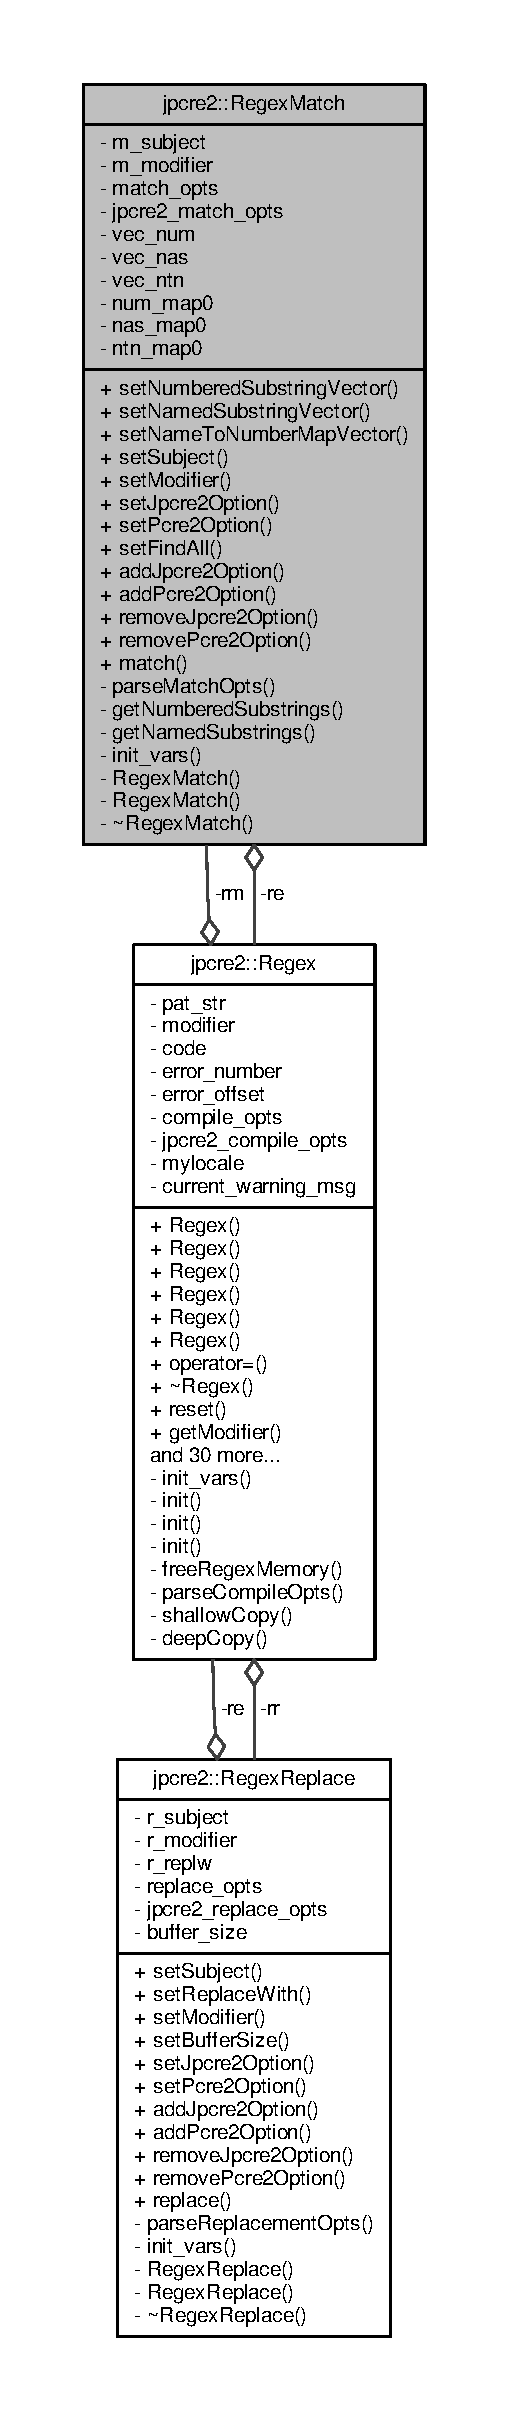
\includegraphics[height=550pt]{classjpcre2_1_1RegexMatch__coll__graph}
\end{center}
\end{figure}
\subsubsection*{Public Member Functions}
\begin{DoxyCompactItemize}
\item 
\hyperlink{classjpcre2_1_1RegexMatch}{Regex\+Match} \& \hyperlink{classjpcre2_1_1RegexMatch_a2c7efe1ec2e13827f670db4ecedcd0a0}{set\+Numbered\+Substring\+Vector} (\hyperlink{namespacejpcre2_ac1cf752c8fbb0be78020be3b80e77ce3}{Vec\+Num} $\ast$v)
\begin{DoxyCompactList}\small\item\em Set a pointer to the numbered substring vector of type \hyperlink{namespacejpcre2_ac1cf752c8fbb0be78020be3b80e77ce3}{jpcre2\+::\+Vec\+Num}. \end{DoxyCompactList}\item 
\hyperlink{classjpcre2_1_1RegexMatch}{Regex\+Match} \& \hyperlink{classjpcre2_1_1RegexMatch_ae495431f57cae54363331237ab21b56c}{set\+Named\+Substring\+Vector} (\hyperlink{namespacejpcre2_a2b121ae776ea5b2913839f418a7d856b}{Vec\+Nas} $\ast$v)
\begin{DoxyCompactList}\small\item\em Set a pointer to the named substring vector of type \hyperlink{namespacejpcre2_a2b121ae776ea5b2913839f418a7d856b}{jpcre2\+::\+Vec\+Nas}. \end{DoxyCompactList}\item 
\hyperlink{classjpcre2_1_1RegexMatch}{Regex\+Match} \& \hyperlink{classjpcre2_1_1RegexMatch_a04926e61d8b5f1d8bdf344efecd567d8}{set\+Name\+To\+Number\+Map\+Vector} (\hyperlink{namespacejpcre2_a88a7aaf84cad627d34c8152e726168eb}{Vec\+NtN} $\ast$v)
\begin{DoxyCompactList}\small\item\em Set a pointer to the name to number map vector of type \hyperlink{namespacejpcre2_a88a7aaf84cad627d34c8152e726168eb}{jpcre2\+::\+Vec\+NtN}. \end{DoxyCompactList}\item 
\hyperlink{classjpcre2_1_1RegexMatch}{Regex\+Match} \& \hyperlink{classjpcre2_1_1RegexMatch_a635c652195deaa8ebb9e107c4f972aab}{set\+Subject} (const \hyperlink{namespacejpcre2_a91f03070152fb228bc116c5a737f1d16}{String} \&s)
\begin{DoxyCompactList}\small\item\em Set the subject string \hyperlink{classjpcre2_1_1RegexMatch_a9df4f1897e7fa33e05a9f6f938992ca7}{m\+\_\+subject}. \end{DoxyCompactList}\item 
\hyperlink{classjpcre2_1_1RegexMatch}{Regex\+Match} \& \hyperlink{classjpcre2_1_1RegexMatch_a9df7e92f96b61553f62720cb8f5f23e5}{set\+Modifier} (const \hyperlink{namespacejpcre2_a91f03070152fb228bc116c5a737f1d16}{String} \&s)
\begin{DoxyCompactList}\small\item\em Set the modifier \hyperlink{classjpcre2_1_1RegexMatch_a5d3e216a4cfc80d00fc45c51a8136821}{m\+\_\+modifier} (overwrites existing J\+P\+C\+R\+E2 and P\+C\+R\+E2 option). \end{DoxyCompactList}\item 
\hyperlink{classjpcre2_1_1RegexMatch}{Regex\+Match} \& \hyperlink{classjpcre2_1_1RegexMatch_a0d76033d9c134caa9ddfc21849603920}{set\+Jpcre2\+Option} (\hyperlink{namespacejpcre2_a078242d38221a13fb3543b9edd78c099}{Uint} x)
\begin{DoxyCompactList}\small\item\em Set J\+P\+C\+R\+E2 option \hyperlink{classjpcre2_1_1RegexMatch_a70d62df887eeed237724f64fbc378700}{jpcre2\+\_\+match\+\_\+opts} (overwrite existing option) \end{DoxyCompactList}\item 
\hyperlink{classjpcre2_1_1RegexMatch}{Regex\+Match} \& \hyperlink{classjpcre2_1_1RegexMatch_ae4ab558c2bec0bc9639dbca70ab47496}{set\+Pcre2\+Option} (\hyperlink{namespacejpcre2_a078242d38221a13fb3543b9edd78c099}{Uint} x)
\begin{DoxyCompactList}\small\item\em Set P\+C\+R\+E2 option \hyperlink{classjpcre2_1_1RegexMatch_a697d5731007350b0f20d2018fcfafa90}{match\+\_\+opts} (overwrite existing option) \end{DoxyCompactList}\item 
\hyperlink{classjpcre2_1_1RegexMatch}{Regex\+Match} \& \hyperlink{classjpcre2_1_1RegexMatch_a85bdec86583f800dafcb1aae27f855e7}{set\+Find\+All} (bool x=true)
\begin{DoxyCompactList}\small\item\em Set whether to perform global match. \end{DoxyCompactList}\item 
\hyperlink{classjpcre2_1_1RegexMatch}{Regex\+Match} \& \hyperlink{classjpcre2_1_1RegexMatch_a0a4cf8554a7e00f3cf2db34f60a43f60}{add\+Jpcre2\+Option} (\hyperlink{namespacejpcre2_a078242d38221a13fb3543b9edd78c099}{Uint} x)
\begin{DoxyCompactList}\small\item\em Add option to existing J\+P\+C\+R\+E2 options \hyperlink{classjpcre2_1_1RegexMatch_a70d62df887eeed237724f64fbc378700}{jpcre2\+\_\+match\+\_\+opts}. \end{DoxyCompactList}\item 
\hyperlink{classjpcre2_1_1RegexMatch}{Regex\+Match} \& \hyperlink{classjpcre2_1_1RegexMatch_aac4857cd8f5eae15b29b9afbe9023522}{add\+Pcre2\+Option} (\hyperlink{namespacejpcre2_a078242d38221a13fb3543b9edd78c099}{Uint} x)
\begin{DoxyCompactList}\small\item\em Add option to existing P\+C\+R\+E2 options \hyperlink{classjpcre2_1_1RegexMatch_a697d5731007350b0f20d2018fcfafa90}{match\+\_\+opts}. \end{DoxyCompactList}\item 
\hyperlink{classjpcre2_1_1RegexMatch}{Regex\+Match} \& \hyperlink{classjpcre2_1_1RegexMatch_a580a64c66ea34153559142928d33d78a}{remove\+Jpcre2\+Option} (\hyperlink{namespacejpcre2_a078242d38221a13fb3543b9edd78c099}{Uint} x)
\begin{DoxyCompactList}\small\item\em Remove option from existing J\+P\+C\+R\+E2 option \hyperlink{classjpcre2_1_1RegexMatch_a70d62df887eeed237724f64fbc378700}{jpcre2\+\_\+match\+\_\+opts}. \end{DoxyCompactList}\item 
\hyperlink{classjpcre2_1_1RegexMatch}{Regex\+Match} \& \hyperlink{classjpcre2_1_1RegexMatch_a1405a2d332d1a928ceb67857097be665}{remove\+Pcre2\+Option} (\hyperlink{namespacejpcre2_a078242d38221a13fb3543b9edd78c099}{Uint} x)
\begin{DoxyCompactList}\small\item\em Remove option from existing P\+C\+R\+E2 option \hyperlink{classjpcre2_1_1RegexMatch_a697d5731007350b0f20d2018fcfafa90}{match\+\_\+opts}. \end{DoxyCompactList}\item 
\hyperlink{namespacejpcre2_a2aac465ddcb123560c7c8215dd69246c}{S\+I\+Z\+E\+\_\+T} \hyperlink{classjpcre2_1_1RegexMatch_a5868aef3a146594ea1ebef34d122bb33}{match} (void)
\begin{DoxyCompactList}\small\item\em Return the number of matches, store the match results in the specified vectors (\hyperlink{classjpcre2_1_1RegexMatch_a836705e0444568c78abaab4c8e351335}{vec\+\_\+num}, \hyperlink{classjpcre2_1_1RegexMatch_a812b57dc08fdc0caa93a1b508ef8242c}{vec\+\_\+nas}, \hyperlink{classjpcre2_1_1RegexMatch_a86ef413ab6d237972af858be26ff77f7}{vec\+\_\+ntn}) \end{DoxyCompactList}\end{DoxyCompactItemize}
\subsubsection*{Private Member Functions}
\begin{DoxyCompactItemize}
\item 
void \hyperlink{classjpcre2_1_1RegexMatch_a5cacfea4b4d3c26307fb10e88e711af3}{parse\+Match\+Opts} (void)
\begin{DoxyCompactList}\small\item\em Parse \hyperlink{classjpcre2_1_1RegexMatch_a5d3e216a4cfc80d00fc45c51a8136821}{m\+\_\+modifier} and set equivalent P\+C\+R\+E2 and J\+P\+C\+R\+E2 options. \end{DoxyCompactList}\item 
void \hyperlink{classjpcre2_1_1RegexMatch_a961a5f91ab24a1ddfd42910c6ab68b65}{get\+Numbered\+Substrings} (int rc, pcre2\+\_\+match\+\_\+data $\ast$match\+\_\+data)\hypertarget{classjpcre2_1_1RegexMatch_a961a5f91ab24a1ddfd42910c6ab68b65}{}\label{classjpcre2_1_1RegexMatch_a961a5f91ab24a1ddfd42910c6ab68b65}

\begin{DoxyCompactList}\small\item\em Populate \hyperlink{classjpcre2_1_1RegexMatch_a94ad930ea8cb22873737fda344bae508}{num\+\_\+map0} with numbered substrings. \end{DoxyCompactList}\item 
void \hyperlink{classjpcre2_1_1RegexMatch_af159e8d080ecd74f63ec67b1d5a27772}{get\+Named\+Substrings} (int namecount, int name\+\_\+entry\+\_\+size, P\+C\+R\+E2\+\_\+\+S\+P\+TR tabptr, pcre2\+\_\+match\+\_\+data $\ast$match\+\_\+data)\hypertarget{classjpcre2_1_1RegexMatch_af159e8d080ecd74f63ec67b1d5a27772}{}\label{classjpcre2_1_1RegexMatch_af159e8d080ecd74f63ec67b1d5a27772}

\begin{DoxyCompactList}\small\item\em Populate \hyperlink{classjpcre2_1_1RegexMatch_a36749947847f266de03c3991ac88a694}{nas\+\_\+map0} and/or \hyperlink{classjpcre2_1_1RegexMatch_a1c790683d023313967ce80db6045419f}{ntn\+\_\+map0} with named substring and/or name to number mapping. \end{DoxyCompactList}\item 
void \hyperlink{classjpcre2_1_1RegexMatch_a3da6a2319cd577d7f2f10c66dcf59a99}{init\+\_\+vars} ()\hypertarget{classjpcre2_1_1RegexMatch_a3da6a2319cd577d7f2f10c66dcf59a99}{}\label{classjpcre2_1_1RegexMatch_a3da6a2319cd577d7f2f10c66dcf59a99}

\begin{DoxyCompactList}\small\item\em Initialize class variables. \end{DoxyCompactList}\item 
\hyperlink{classjpcre2_1_1RegexMatch_a40127e5057e2343848d8c8a6d4c32bcd}{Regex\+Match} ()
\begin{DoxyCompactList}\small\item\em Default constructor. \end{DoxyCompactList}\item 
\hyperlink{classjpcre2_1_1RegexMatch_a098ddb46b2f297870ea548ef07597d94}{Regex\+Match} (const \hyperlink{classjpcre2_1_1RegexMatch}{Regex\+Match} \&)
\begin{DoxyCompactList}\small\item\em This is a copy constructor which is only used to prevent public object creation. \end{DoxyCompactList}\item 
\hyperlink{classjpcre2_1_1RegexMatch_ab6a9f9b8404852e46edd08a5b8712847}{$\sim$\+Regex\+Match} ()
\begin{DoxyCompactList}\small\item\em Destructor. \end{DoxyCompactList}\end{DoxyCompactItemize}
\subsubsection*{Private Attributes}
\begin{DoxyCompactItemize}
\item 
\hyperlink{classjpcre2_1_1Regex}{Regex} $\ast$ \hyperlink{classjpcre2_1_1RegexMatch_a7743b27db00c1e13d8fee51b70d5a133}{re}\hypertarget{classjpcre2_1_1RegexMatch_a7743b27db00c1e13d8fee51b70d5a133}{}\label{classjpcre2_1_1RegexMatch_a7743b27db00c1e13d8fee51b70d5a133}

\begin{DoxyCompactList}\small\item\em This is used to access private members in \hyperlink{classjpcre2_1_1Regex}{Regex}. \end{DoxyCompactList}\item 
\hyperlink{namespacejpcre2_a91f03070152fb228bc116c5a737f1d16}{String} \hyperlink{classjpcre2_1_1RegexMatch_a9df4f1897e7fa33e05a9f6f938992ca7}{m\+\_\+subject}\hypertarget{classjpcre2_1_1RegexMatch_a9df4f1897e7fa33e05a9f6f938992ca7}{}\label{classjpcre2_1_1RegexMatch_a9df4f1897e7fa33e05a9f6f938992ca7}

\begin{DoxyCompactList}\small\item\em Subject string for match. \end{DoxyCompactList}\item 
\hyperlink{namespacejpcre2_a91f03070152fb228bc116c5a737f1d16}{String} \hyperlink{classjpcre2_1_1RegexMatch_a5d3e216a4cfc80d00fc45c51a8136821}{m\+\_\+modifier}\hypertarget{classjpcre2_1_1RegexMatch_a5d3e216a4cfc80d00fc45c51a8136821}{}\label{classjpcre2_1_1RegexMatch_a5d3e216a4cfc80d00fc45c51a8136821}

\begin{DoxyCompactList}\small\item\em Pattern for match. \end{DoxyCompactList}\item 
\hyperlink{namespacejpcre2_a078242d38221a13fb3543b9edd78c099}{Uint} \hyperlink{classjpcre2_1_1RegexMatch_a697d5731007350b0f20d2018fcfafa90}{match\+\_\+opts}\hypertarget{classjpcre2_1_1RegexMatch_a697d5731007350b0f20d2018fcfafa90}{}\label{classjpcre2_1_1RegexMatch_a697d5731007350b0f20d2018fcfafa90}

\begin{DoxyCompactList}\small\item\em P\+C\+R\+E2 options for pcre2\+\_\+match() (P\+C\+R\+E2 internal function) \end{DoxyCompactList}\item 
\hyperlink{namespacejpcre2_a078242d38221a13fb3543b9edd78c099}{Uint} \hyperlink{classjpcre2_1_1RegexMatch_a70d62df887eeed237724f64fbc378700}{jpcre2\+\_\+match\+\_\+opts}\hypertarget{classjpcre2_1_1RegexMatch_a70d62df887eeed237724f64fbc378700}{}\label{classjpcre2_1_1RegexMatch_a70d62df887eeed237724f64fbc378700}

\begin{DoxyCompactList}\small\item\em J\+P\+C\+R\+E2 options for match. \end{DoxyCompactList}\item 
\hyperlink{namespacejpcre2_ac1cf752c8fbb0be78020be3b80e77ce3}{Vec\+Num} $\ast$ \hyperlink{classjpcre2_1_1RegexMatch_a836705e0444568c78abaab4c8e351335}{vec\+\_\+num}\hypertarget{classjpcre2_1_1RegexMatch_a836705e0444568c78abaab4c8e351335}{}\label{classjpcre2_1_1RegexMatch_a836705e0444568c78abaab4c8e351335}

\begin{DoxyCompactList}\small\item\em Pointer to vector that will store the numbered substring maps. \end{DoxyCompactList}\item 
\hyperlink{namespacejpcre2_a2b121ae776ea5b2913839f418a7d856b}{Vec\+Nas} $\ast$ \hyperlink{classjpcre2_1_1RegexMatch_a812b57dc08fdc0caa93a1b508ef8242c}{vec\+\_\+nas}\hypertarget{classjpcre2_1_1RegexMatch_a812b57dc08fdc0caa93a1b508ef8242c}{}\label{classjpcre2_1_1RegexMatch_a812b57dc08fdc0caa93a1b508ef8242c}

\begin{DoxyCompactList}\small\item\em Pointer to vector that will store the named substring maps. \end{DoxyCompactList}\item 
\hyperlink{namespacejpcre2_a88a7aaf84cad627d34c8152e726168eb}{Vec\+NtN} $\ast$ \hyperlink{classjpcre2_1_1RegexMatch_a86ef413ab6d237972af858be26ff77f7}{vec\+\_\+ntn}\hypertarget{classjpcre2_1_1RegexMatch_a86ef413ab6d237972af858be26ff77f7}{}\label{classjpcre2_1_1RegexMatch_a86ef413ab6d237972af858be26ff77f7}

\begin{DoxyCompactList}\small\item\em Pointer to vector that will store the name to number maps. \end{DoxyCompactList}\item 
\hyperlink{namespacejpcre2_a947e37f0e4a1678157e7f1f855638e82}{Map\+Num} $\ast$ \hyperlink{classjpcre2_1_1RegexMatch_a94ad930ea8cb22873737fda344bae508}{num\+\_\+map0}\hypertarget{classjpcre2_1_1RegexMatch_a94ad930ea8cb22873737fda344bae508}{}\label{classjpcre2_1_1RegexMatch_a94ad930ea8cb22873737fda344bae508}

\begin{DoxyCompactList}\small\item\em Pointer to map that will store numbered substrings temporarily. \end{DoxyCompactList}\item 
\hyperlink{namespacejpcre2_a20bd901c9ca3c949806aa6b9e324f6cf}{Map\+Nas} $\ast$ \hyperlink{classjpcre2_1_1RegexMatch_a36749947847f266de03c3991ac88a694}{nas\+\_\+map0}\hypertarget{classjpcre2_1_1RegexMatch_a36749947847f266de03c3991ac88a694}{}\label{classjpcre2_1_1RegexMatch_a36749947847f266de03c3991ac88a694}

\begin{DoxyCompactList}\small\item\em Pointer to map that will store named substrings temporarily. \end{DoxyCompactList}\item 
\hyperlink{namespacejpcre2_a753ebedfb8caf4a16ffbf47d8d705656}{Map\+NtN} $\ast$ \hyperlink{classjpcre2_1_1RegexMatch_a1c790683d023313967ce80db6045419f}{ntn\+\_\+map0}\hypertarget{classjpcre2_1_1RegexMatch_a1c790683d023313967ce80db6045419f}{}\label{classjpcre2_1_1RegexMatch_a1c790683d023313967ce80db6045419f}

\begin{DoxyCompactList}\small\item\em Pointer to map that will store name to number mapping temporarily. \end{DoxyCompactList}\end{DoxyCompactItemize}
\subsubsection*{Friends}
\begin{DoxyCompactItemize}
\item 
class \hyperlink{classjpcre2_1_1RegexMatch_a1f6f7620b7d2218c6c2a6a47f432ea6a}{Regex}\hypertarget{classjpcre2_1_1RegexMatch_a1f6f7620b7d2218c6c2a6a47f432ea6a}{}\label{classjpcre2_1_1RegexMatch_a1f6f7620b7d2218c6c2a6a47f432ea6a}

\begin{DoxyCompactList}\small\item\em Define class \hyperlink{classjpcre2_1_1Regex}{Regex} as friend and thus allow \hyperlink{classjpcre2_1_1Regex}{Regex} to create object of this class. \end{DoxyCompactList}\end{DoxyCompactItemize}


\subsubsection{Detailed Description}
Performs regex matching. 

Provides chained methods to set various options.

All constructors of this class are private. 

\subsubsection{Constructor \& Destructor Documentation}
\index{jpcre2\+::\+Regex\+Match@{jpcre2\+::\+Regex\+Match}!Regex\+Match@{Regex\+Match}}
\index{Regex\+Match@{Regex\+Match}!jpcre2\+::\+Regex\+Match@{jpcre2\+::\+Regex\+Match}}
\paragraph[{\texorpdfstring{Regex\+Match()}{RegexMatch()}}]{\setlength{\rightskip}{0pt plus 5cm}jpcre2\+::\+Regex\+Match\+::\+Regex\+Match (
\begin{DoxyParamCaption}
{}
\end{DoxyParamCaption}
)\hspace{0.3cm}{\ttfamily [inline]}, {\ttfamily [private]}}\hypertarget{classjpcre2_1_1RegexMatch_a40127e5057e2343848d8c8a6d4c32bcd}{}\label{classjpcre2_1_1RegexMatch_a40127e5057e2343848d8c8a6d4c32bcd}


Default constructor. 

Initialize class variables. \index{jpcre2\+::\+Regex\+Match@{jpcre2\+::\+Regex\+Match}!Regex\+Match@{Regex\+Match}}
\index{Regex\+Match@{Regex\+Match}!jpcre2\+::\+Regex\+Match@{jpcre2\+::\+Regex\+Match}}
\paragraph[{\texorpdfstring{Regex\+Match(const Regex\+Match \&)}{RegexMatch(const RegexMatch &)}}]{\setlength{\rightskip}{0pt plus 5cm}jpcre2\+::\+Regex\+Match\+::\+Regex\+Match (
\begin{DoxyParamCaption}
\item[{const {\bf Regex\+Match} \&}]{}
\end{DoxyParamCaption}
)\hspace{0.3cm}{\ttfamily [inline]}, {\ttfamily [private]}}\hypertarget{classjpcre2_1_1RegexMatch_a098ddb46b2f297870ea548ef07597d94}{}\label{classjpcre2_1_1RegexMatch_a098ddb46b2f297870ea548ef07597d94}


This is a copy constructor which is only used to prevent public object creation. 

No need to implement it completely \index{jpcre2\+::\+Regex\+Match@{jpcre2\+::\+Regex\+Match}!````~Regex\+Match@{$\sim$\+Regex\+Match}}
\index{````~Regex\+Match@{$\sim$\+Regex\+Match}!jpcre2\+::\+Regex\+Match@{jpcre2\+::\+Regex\+Match}}
\paragraph[{\texorpdfstring{$\sim$\+Regex\+Match()}{~RegexMatch()}}]{\setlength{\rightskip}{0pt plus 5cm}jpcre2\+::\+Regex\+Match\+::$\sim$\+Regex\+Match (
\begin{DoxyParamCaption}
{}
\end{DoxyParamCaption}
)\hspace{0.3cm}{\ttfamily [inline]}, {\ttfamily [private]}}\hypertarget{classjpcre2_1_1RegexMatch_ab6a9f9b8404852e46edd08a5b8712847}{}\label{classjpcre2_1_1RegexMatch_ab6a9f9b8404852e46edd08a5b8712847}


Destructor. 

Deletes the temporary maps that were created to store substrings 

\subsubsection{Member Function Documentation}
\index{jpcre2\+::\+Regex\+Match@{jpcre2\+::\+Regex\+Match}!add\+Jpcre2\+Option@{add\+Jpcre2\+Option}}
\index{add\+Jpcre2\+Option@{add\+Jpcre2\+Option}!jpcre2\+::\+Regex\+Match@{jpcre2\+::\+Regex\+Match}}
\paragraph[{\texorpdfstring{add\+Jpcre2\+Option(\+Uint x)}{addJpcre2Option(Uint x)}}]{\setlength{\rightskip}{0pt plus 5cm}{\bf Regex\+Match}\& jpcre2\+::\+Regex\+Match\+::add\+Jpcre2\+Option (
\begin{DoxyParamCaption}
\item[{{\bf Uint}}]{x}
\end{DoxyParamCaption}
)\hspace{0.3cm}{\ttfamily [inline]}}\hypertarget{classjpcre2_1_1RegexMatch_a0a4cf8554a7e00f3cf2db34f60a43f60}{}\label{classjpcre2_1_1RegexMatch_a0a4cf8554a7e00f3cf2db34f60a43f60}


Add option to existing J\+P\+C\+R\+E2 options \hyperlink{classjpcre2_1_1RegexMatch_a70d62df887eeed237724f64fbc378700}{jpcre2\+\_\+match\+\_\+opts}. 


\begin{DoxyParams}{Parameters}
{\em x} & Option value \\
\hline
\end{DoxyParams}
\begin{DoxyReturn}{Returns}
$\ast$this 
\end{DoxyReturn}
\index{jpcre2\+::\+Regex\+Match@{jpcre2\+::\+Regex\+Match}!add\+Pcre2\+Option@{add\+Pcre2\+Option}}
\index{add\+Pcre2\+Option@{add\+Pcre2\+Option}!jpcre2\+::\+Regex\+Match@{jpcre2\+::\+Regex\+Match}}
\paragraph[{\texorpdfstring{add\+Pcre2\+Option(\+Uint x)}{addPcre2Option(Uint x)}}]{\setlength{\rightskip}{0pt plus 5cm}{\bf Regex\+Match}\& jpcre2\+::\+Regex\+Match\+::add\+Pcre2\+Option (
\begin{DoxyParamCaption}
\item[{{\bf Uint}}]{x}
\end{DoxyParamCaption}
)\hspace{0.3cm}{\ttfamily [inline]}}\hypertarget{classjpcre2_1_1RegexMatch_aac4857cd8f5eae15b29b9afbe9023522}{}\label{classjpcre2_1_1RegexMatch_aac4857cd8f5eae15b29b9afbe9023522}


Add option to existing P\+C\+R\+E2 options \hyperlink{classjpcre2_1_1RegexMatch_a697d5731007350b0f20d2018fcfafa90}{match\+\_\+opts}. 


\begin{DoxyParams}{Parameters}
{\em x} & Option value \\
\hline
\end{DoxyParams}
\begin{DoxyReturn}{Returns}
$\ast$this 
\end{DoxyReturn}
\index{jpcre2\+::\+Regex\+Match@{jpcre2\+::\+Regex\+Match}!match@{match}}
\index{match@{match}!jpcre2\+::\+Regex\+Match@{jpcre2\+::\+Regex\+Match}}
\paragraph[{\texorpdfstring{match(void)}{match(void)}}]{\setlength{\rightskip}{0pt plus 5cm}{\bf jpcre2\+::\+S\+I\+Z\+E\+\_\+T} jpcre2\+::\+Regex\+Match\+::match (
\begin{DoxyParamCaption}
\item[{void}]{}
\end{DoxyParamCaption}
)}\hypertarget{classjpcre2_1_1RegexMatch_a5868aef3a146594ea1ebef34d122bb33}{}\label{classjpcre2_1_1RegexMatch_a5868aef3a146594ea1ebef34d122bb33}


Return the number of matches, store the match results in the specified vectors (\hyperlink{classjpcre2_1_1RegexMatch_a836705e0444568c78abaab4c8e351335}{vec\+\_\+num}, \hyperlink{classjpcre2_1_1RegexMatch_a812b57dc08fdc0caa93a1b508ef8242c}{vec\+\_\+nas}, \hyperlink{classjpcre2_1_1RegexMatch_a86ef413ab6d237972af858be26ff77f7}{vec\+\_\+ntn}) 

\begin{DoxyReturn}{Returns}
Number of matches found 
\end{DoxyReturn}
\begin{DoxySeeAlso}{See also}
\hyperlink{namespacejpcre2_a2aac465ddcb123560c7c8215dd69246c}{S\+I\+Z\+E\+\_\+T} match(const String\& s) 

\hyperlink{namespacejpcre2_a2aac465ddcb123560c7c8215dd69246c}{S\+I\+Z\+E\+\_\+T} match(const String\& s, const String\& mod) 
\end{DoxySeeAlso}


References jpcre2\+::\+F\+I\+N\+D\+\_\+\+A\+LL.



Referenced by jpcre2\+::\+Regex\+::match().



Here is the caller graph for this function\+:
\nopagebreak
\begin{figure}[H]
\begin{center}
\leavevmode
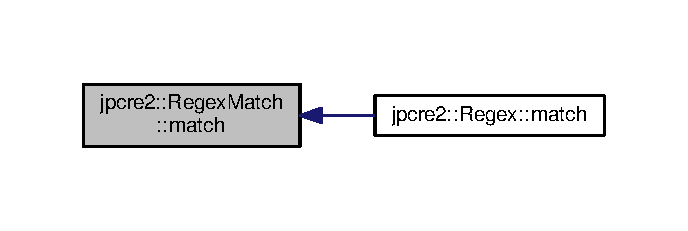
\includegraphics[width=330pt]{classjpcre2_1_1RegexMatch_a5868aef3a146594ea1ebef34d122bb33_icgraph}
\end{center}
\end{figure}


\index{jpcre2\+::\+Regex\+Match@{jpcre2\+::\+Regex\+Match}!parse\+Match\+Opts@{parse\+Match\+Opts}}
\index{parse\+Match\+Opts@{parse\+Match\+Opts}!jpcre2\+::\+Regex\+Match@{jpcre2\+::\+Regex\+Match}}
\paragraph[{\texorpdfstring{parse\+Match\+Opts(void)}{parseMatchOpts(void)}}]{\setlength{\rightskip}{0pt plus 5cm}void jpcre2\+::\+Regex\+Match\+::parse\+Match\+Opts (
\begin{DoxyParamCaption}
\item[{void}]{}
\end{DoxyParamCaption}
)\hspace{0.3cm}{\ttfamily [private]}}\hypertarget{classjpcre2_1_1RegexMatch_a5cacfea4b4d3c26307fb10e88e711af3}{}\label{classjpcre2_1_1RegexMatch_a5cacfea4b4d3c26307fb10e88e711af3}


Parse \hyperlink{classjpcre2_1_1RegexMatch_a5d3e216a4cfc80d00fc45c51a8136821}{m\+\_\+modifier} and set equivalent P\+C\+R\+E2 and J\+P\+C\+R\+E2 options. 

After a call to this function \hyperlink{classjpcre2_1_1RegexMatch_a697d5731007350b0f20d2018fcfafa90}{match\+\_\+opts} and \hyperlink{classjpcre2_1_1RegexMatch_a70d62df887eeed237724f64fbc378700}{jpcre2\+\_\+match\+\_\+opts} will be properly set. 

References jpcre2\+::\+F\+I\+N\+D\+\_\+\+A\+LL, jpcre2\+::\+E\+R\+R\+O\+R\+::\+I\+N\+V\+A\+L\+I\+D\+\_\+\+M\+O\+D\+I\+F\+I\+ER, and jpcre2\+::\+V\+A\+L\+I\+D\+A\+T\+E\+\_\+\+M\+O\+D\+I\+F\+I\+ER.

\index{jpcre2\+::\+Regex\+Match@{jpcre2\+::\+Regex\+Match}!remove\+Jpcre2\+Option@{remove\+Jpcre2\+Option}}
\index{remove\+Jpcre2\+Option@{remove\+Jpcre2\+Option}!jpcre2\+::\+Regex\+Match@{jpcre2\+::\+Regex\+Match}}
\paragraph[{\texorpdfstring{remove\+Jpcre2\+Option(\+Uint x)}{removeJpcre2Option(Uint x)}}]{\setlength{\rightskip}{0pt plus 5cm}{\bf Regex\+Match}\& jpcre2\+::\+Regex\+Match\+::remove\+Jpcre2\+Option (
\begin{DoxyParamCaption}
\item[{{\bf Uint}}]{x}
\end{DoxyParamCaption}
)\hspace{0.3cm}{\ttfamily [inline]}}\hypertarget{classjpcre2_1_1RegexMatch_a580a64c66ea34153559142928d33d78a}{}\label{classjpcre2_1_1RegexMatch_a580a64c66ea34153559142928d33d78a}


Remove option from existing J\+P\+C\+R\+E2 option \hyperlink{classjpcre2_1_1RegexMatch_a70d62df887eeed237724f64fbc378700}{jpcre2\+\_\+match\+\_\+opts}. 


\begin{DoxyParams}{Parameters}
{\em x} & Option value \\
\hline
\end{DoxyParams}
\begin{DoxyReturn}{Returns}
$\ast$this 
\end{DoxyReturn}
\index{jpcre2\+::\+Regex\+Match@{jpcre2\+::\+Regex\+Match}!remove\+Pcre2\+Option@{remove\+Pcre2\+Option}}
\index{remove\+Pcre2\+Option@{remove\+Pcre2\+Option}!jpcre2\+::\+Regex\+Match@{jpcre2\+::\+Regex\+Match}}
\paragraph[{\texorpdfstring{remove\+Pcre2\+Option(\+Uint x)}{removePcre2Option(Uint x)}}]{\setlength{\rightskip}{0pt plus 5cm}{\bf Regex\+Match}\& jpcre2\+::\+Regex\+Match\+::remove\+Pcre2\+Option (
\begin{DoxyParamCaption}
\item[{{\bf Uint}}]{x}
\end{DoxyParamCaption}
)\hspace{0.3cm}{\ttfamily [inline]}}\hypertarget{classjpcre2_1_1RegexMatch_a1405a2d332d1a928ceb67857097be665}{}\label{classjpcre2_1_1RegexMatch_a1405a2d332d1a928ceb67857097be665}


Remove option from existing P\+C\+R\+E2 option \hyperlink{classjpcre2_1_1RegexMatch_a697d5731007350b0f20d2018fcfafa90}{match\+\_\+opts}. 


\begin{DoxyParams}{Parameters}
{\em x} & Option value \\
\hline
\end{DoxyParams}
\begin{DoxyReturn}{Returns}
$\ast$this 
\end{DoxyReturn}
\index{jpcre2\+::\+Regex\+Match@{jpcre2\+::\+Regex\+Match}!set\+Find\+All@{set\+Find\+All}}
\index{set\+Find\+All@{set\+Find\+All}!jpcre2\+::\+Regex\+Match@{jpcre2\+::\+Regex\+Match}}
\paragraph[{\texorpdfstring{set\+Find\+All(bool x=true)}{setFindAll(bool x=true)}}]{\setlength{\rightskip}{0pt plus 5cm}{\bf Regex\+Match}\& jpcre2\+::\+Regex\+Match\+::set\+Find\+All (
\begin{DoxyParamCaption}
\item[{bool}]{x = {\ttfamily true}}
\end{DoxyParamCaption}
)\hspace{0.3cm}{\ttfamily [inline]}}\hypertarget{classjpcre2_1_1RegexMatch_a85bdec86583f800dafcb1aae27f855e7}{}\label{classjpcre2_1_1RegexMatch_a85bdec86583f800dafcb1aae27f855e7}


Set whether to perform global match. 


\begin{DoxyParams}{Parameters}
{\em x} & True or False \\
\hline
\end{DoxyParams}
\begin{DoxyReturn}{Returns}
$\ast$this 
\end{DoxyReturn}


References jpcre2\+::\+F\+I\+N\+D\+\_\+\+A\+LL.

\index{jpcre2\+::\+Regex\+Match@{jpcre2\+::\+Regex\+Match}!set\+Jpcre2\+Option@{set\+Jpcre2\+Option}}
\index{set\+Jpcre2\+Option@{set\+Jpcre2\+Option}!jpcre2\+::\+Regex\+Match@{jpcre2\+::\+Regex\+Match}}
\paragraph[{\texorpdfstring{set\+Jpcre2\+Option(\+Uint x)}{setJpcre2Option(Uint x)}}]{\setlength{\rightskip}{0pt plus 5cm}{\bf Regex\+Match}\& jpcre2\+::\+Regex\+Match\+::set\+Jpcre2\+Option (
\begin{DoxyParamCaption}
\item[{{\bf Uint}}]{x}
\end{DoxyParamCaption}
)\hspace{0.3cm}{\ttfamily [inline]}}\hypertarget{classjpcre2_1_1RegexMatch_a0d76033d9c134caa9ddfc21849603920}{}\label{classjpcre2_1_1RegexMatch_a0d76033d9c134caa9ddfc21849603920}


Set J\+P\+C\+R\+E2 option \hyperlink{classjpcre2_1_1RegexMatch_a70d62df887eeed237724f64fbc378700}{jpcre2\+\_\+match\+\_\+opts} (overwrite existing option) 


\begin{DoxyParams}{Parameters}
{\em x} & Option value \\
\hline
\end{DoxyParams}
\begin{DoxyReturn}{Returns}
$\ast$this 
\end{DoxyReturn}
\index{jpcre2\+::\+Regex\+Match@{jpcre2\+::\+Regex\+Match}!set\+Modifier@{set\+Modifier}}
\index{set\+Modifier@{set\+Modifier}!jpcre2\+::\+Regex\+Match@{jpcre2\+::\+Regex\+Match}}
\paragraph[{\texorpdfstring{set\+Modifier(const String \&s)}{setModifier(const String &s)}}]{\setlength{\rightskip}{0pt plus 5cm}{\bf Regex\+Match}\& jpcre2\+::\+Regex\+Match\+::set\+Modifier (
\begin{DoxyParamCaption}
\item[{const {\bf String} \&}]{s}
\end{DoxyParamCaption}
)\hspace{0.3cm}{\ttfamily [inline]}}\hypertarget{classjpcre2_1_1RegexMatch_a9df7e92f96b61553f62720cb8f5f23e5}{}\label{classjpcre2_1_1RegexMatch_a9df7e92f96b61553f62720cb8f5f23e5}


Set the modifier \hyperlink{classjpcre2_1_1RegexMatch_a5d3e216a4cfc80d00fc45c51a8136821}{m\+\_\+modifier} (overwrites existing J\+P\+C\+R\+E2 and P\+C\+R\+E2 option). 

Re-\/initializes the option bits for P\+C\+R\+E2 and J\+P\+C\+R\+E2 options, then sets the modifier. 
\begin{DoxyParams}{Parameters}
{\em s} & Modifier string \\
\hline
\end{DoxyParams}
\begin{DoxyReturn}{Returns}
$\ast$this 
\end{DoxyReturn}


Referenced by jpcre2\+::\+Regex\+::match().



Here is the caller graph for this function\+:
\nopagebreak
\begin{figure}[H]
\begin{center}
\leavevmode
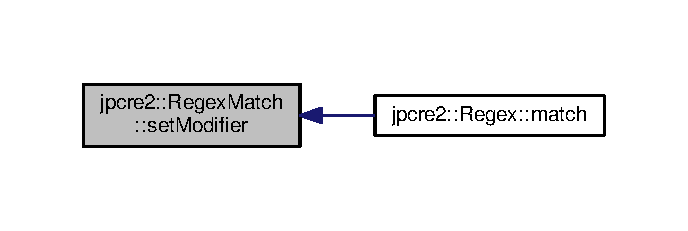
\includegraphics[width=330pt]{classjpcre2_1_1RegexMatch_a9df7e92f96b61553f62720cb8f5f23e5_icgraph}
\end{center}
\end{figure}


\index{jpcre2\+::\+Regex\+Match@{jpcre2\+::\+Regex\+Match}!set\+Named\+Substring\+Vector@{set\+Named\+Substring\+Vector}}
\index{set\+Named\+Substring\+Vector@{set\+Named\+Substring\+Vector}!jpcre2\+::\+Regex\+Match@{jpcre2\+::\+Regex\+Match}}
\paragraph[{\texorpdfstring{set\+Named\+Substring\+Vector(\+Vec\+Nas $\ast$v)}{setNamedSubstringVector(VecNas *v)}}]{\setlength{\rightskip}{0pt plus 5cm}{\bf Regex\+Match}\& jpcre2\+::\+Regex\+Match\+::set\+Named\+Substring\+Vector (
\begin{DoxyParamCaption}
\item[{{\bf Vec\+Nas} $\ast$}]{v}
\end{DoxyParamCaption}
)\hspace{0.3cm}{\ttfamily [inline]}}\hypertarget{classjpcre2_1_1RegexMatch_ae495431f57cae54363331237ab21b56c}{}\label{classjpcre2_1_1RegexMatch_ae495431f57cae54363331237ab21b56c}


Set a pointer to the named substring vector of type \hyperlink{namespacejpcre2_a2b121ae776ea5b2913839f418a7d856b}{jpcre2\+::\+Vec\+Nas}. 


\begin{DoxyParams}{Parameters}
{\em v} & \hyperlink{classjpcre2_1_1RegexMatch_a812b57dc08fdc0caa93a1b508ef8242c}{vec\+\_\+nas} \\
\hline
\end{DoxyParams}
\begin{DoxyReturn}{Returns}
$\ast$this 
\end{DoxyReturn}
\index{jpcre2\+::\+Regex\+Match@{jpcre2\+::\+Regex\+Match}!set\+Name\+To\+Number\+Map\+Vector@{set\+Name\+To\+Number\+Map\+Vector}}
\index{set\+Name\+To\+Number\+Map\+Vector@{set\+Name\+To\+Number\+Map\+Vector}!jpcre2\+::\+Regex\+Match@{jpcre2\+::\+Regex\+Match}}
\paragraph[{\texorpdfstring{set\+Name\+To\+Number\+Map\+Vector(\+Vec\+Nt\+N $\ast$v)}{setNameToNumberMapVector(VecNtN *v)}}]{\setlength{\rightskip}{0pt plus 5cm}{\bf Regex\+Match}\& jpcre2\+::\+Regex\+Match\+::set\+Name\+To\+Number\+Map\+Vector (
\begin{DoxyParamCaption}
\item[{{\bf Vec\+NtN} $\ast$}]{v}
\end{DoxyParamCaption}
)\hspace{0.3cm}{\ttfamily [inline]}}\hypertarget{classjpcre2_1_1RegexMatch_a04926e61d8b5f1d8bdf344efecd567d8}{}\label{classjpcre2_1_1RegexMatch_a04926e61d8b5f1d8bdf344efecd567d8}


Set a pointer to the name to number map vector of type \hyperlink{namespacejpcre2_a88a7aaf84cad627d34c8152e726168eb}{jpcre2\+::\+Vec\+NtN}. 


\begin{DoxyParams}{Parameters}
{\em v} & \hyperlink{classjpcre2_1_1RegexMatch_a86ef413ab6d237972af858be26ff77f7}{vec\+\_\+ntn} \\
\hline
\end{DoxyParams}
\begin{DoxyReturn}{Returns}
$\ast$this 
\end{DoxyReturn}
\index{jpcre2\+::\+Regex\+Match@{jpcre2\+::\+Regex\+Match}!set\+Numbered\+Substring\+Vector@{set\+Numbered\+Substring\+Vector}}
\index{set\+Numbered\+Substring\+Vector@{set\+Numbered\+Substring\+Vector}!jpcre2\+::\+Regex\+Match@{jpcre2\+::\+Regex\+Match}}
\paragraph[{\texorpdfstring{set\+Numbered\+Substring\+Vector(\+Vec\+Num $\ast$v)}{setNumberedSubstringVector(VecNum *v)}}]{\setlength{\rightskip}{0pt plus 5cm}{\bf Regex\+Match}\& jpcre2\+::\+Regex\+Match\+::set\+Numbered\+Substring\+Vector (
\begin{DoxyParamCaption}
\item[{{\bf Vec\+Num} $\ast$}]{v}
\end{DoxyParamCaption}
)\hspace{0.3cm}{\ttfamily [inline]}}\hypertarget{classjpcre2_1_1RegexMatch_a2c7efe1ec2e13827f670db4ecedcd0a0}{}\label{classjpcre2_1_1RegexMatch_a2c7efe1ec2e13827f670db4ecedcd0a0}


Set a pointer to the numbered substring vector of type \hyperlink{namespacejpcre2_ac1cf752c8fbb0be78020be3b80e77ce3}{jpcre2\+::\+Vec\+Num}. 


\begin{DoxyParams}{Parameters}
{\em v} & \hyperlink{classjpcre2_1_1RegexMatch_a836705e0444568c78abaab4c8e351335}{vec\+\_\+num} \\
\hline
\end{DoxyParams}
\begin{DoxyReturn}{Returns}
$\ast$this 
\end{DoxyReturn}
\index{jpcre2\+::\+Regex\+Match@{jpcre2\+::\+Regex\+Match}!set\+Pcre2\+Option@{set\+Pcre2\+Option}}
\index{set\+Pcre2\+Option@{set\+Pcre2\+Option}!jpcre2\+::\+Regex\+Match@{jpcre2\+::\+Regex\+Match}}
\paragraph[{\texorpdfstring{set\+Pcre2\+Option(\+Uint x)}{setPcre2Option(Uint x)}}]{\setlength{\rightskip}{0pt plus 5cm}{\bf Regex\+Match}\& jpcre2\+::\+Regex\+Match\+::set\+Pcre2\+Option (
\begin{DoxyParamCaption}
\item[{{\bf Uint}}]{x}
\end{DoxyParamCaption}
)\hspace{0.3cm}{\ttfamily [inline]}}\hypertarget{classjpcre2_1_1RegexMatch_ae4ab558c2bec0bc9639dbca70ab47496}{}\label{classjpcre2_1_1RegexMatch_ae4ab558c2bec0bc9639dbca70ab47496}


Set P\+C\+R\+E2 option \hyperlink{classjpcre2_1_1RegexMatch_a697d5731007350b0f20d2018fcfafa90}{match\+\_\+opts} (overwrite existing option) 


\begin{DoxyParams}{Parameters}
{\em x} & Option value \\
\hline
\end{DoxyParams}
\begin{DoxyReturn}{Returns}
$\ast$this 
\end{DoxyReturn}
\index{jpcre2\+::\+Regex\+Match@{jpcre2\+::\+Regex\+Match}!set\+Subject@{set\+Subject}}
\index{set\+Subject@{set\+Subject}!jpcre2\+::\+Regex\+Match@{jpcre2\+::\+Regex\+Match}}
\paragraph[{\texorpdfstring{set\+Subject(const String \&s)}{setSubject(const String &s)}}]{\setlength{\rightskip}{0pt plus 5cm}{\bf Regex\+Match}\& jpcre2\+::\+Regex\+Match\+::set\+Subject (
\begin{DoxyParamCaption}
\item[{const {\bf String} \&}]{s}
\end{DoxyParamCaption}
)\hspace{0.3cm}{\ttfamily [inline]}}\hypertarget{classjpcre2_1_1RegexMatch_a635c652195deaa8ebb9e107c4f972aab}{}\label{classjpcre2_1_1RegexMatch_a635c652195deaa8ebb9e107c4f972aab}


Set the subject string \hyperlink{classjpcre2_1_1RegexMatch_a9df4f1897e7fa33e05a9f6f938992ca7}{m\+\_\+subject}. 


\begin{DoxyParams}{Parameters}
{\em s} & Subject string \\
\hline
\end{DoxyParams}
\begin{DoxyReturn}{Returns}
$\ast$this 
\end{DoxyReturn}


Referenced by jpcre2\+::\+Regex\+::match().



Here is the caller graph for this function\+:
\nopagebreak
\begin{figure}[H]
\begin{center}
\leavevmode
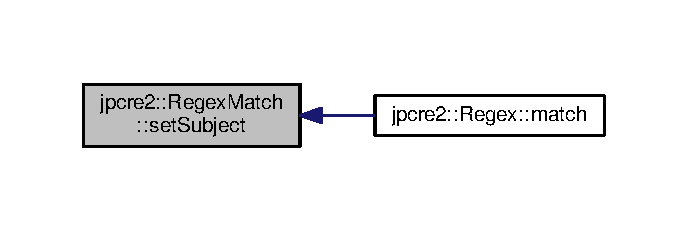
\includegraphics[width=330pt]{classjpcre2_1_1RegexMatch_a635c652195deaa8ebb9e107c4f972aab_icgraph}
\end{center}
\end{figure}




The documentation for this class was generated from the following files\+:\begin{DoxyCompactItemize}
\item 
\hyperlink{jpcre2_8hpp}{jpcre2.\+hpp}\item 
jpcre2.\+cpp\end{DoxyCompactItemize}

\hypertarget{classjpcre2_1_1RegexReplace}{}\subsection{jpcre2\+:\+:Regex\+Replace Class Reference}
\label{classjpcre2_1_1RegexReplace}\index{jpcre2\+::\+Regex\+Replace@{jpcre2\+::\+Regex\+Replace}}


Provides the \hyperlink{classjpcre2_1_1RegexReplace_afd087fa7a9bfedec802d1a3dd7edbdd0}{Regex\+Replace\+::replace()} function to perform regex replace on a string.  




{\ttfamily \#include $<$jpcre2.\+hpp$>$}



Collaboration diagram for jpcre2\+:\+:Regex\+Replace\+:\nopagebreak
\begin{figure}[H]
\begin{center}
\leavevmode
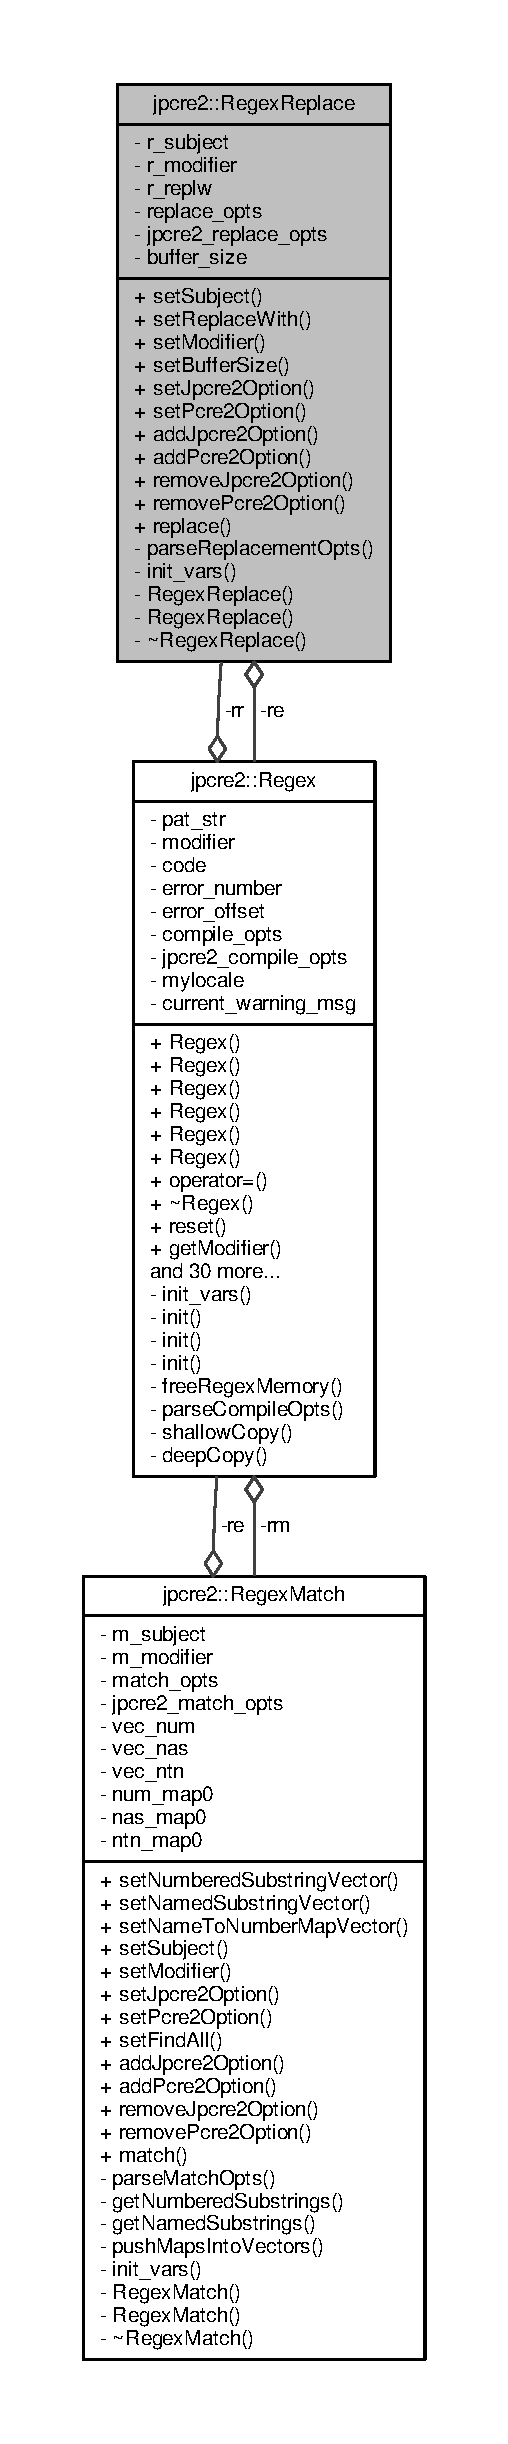
\includegraphics[height=550pt]{classjpcre2_1_1RegexReplace__coll__graph}
\end{center}
\end{figure}
\subsubsection*{Public Member Functions}
\begin{DoxyCompactItemize}
\item 
\hyperlink{classjpcre2_1_1RegexReplace}{Regex\+Replace} \& \hyperlink{classjpcre2_1_1RegexReplace_a46eefdb105827920bebc8436721fa4cb}{set\+Subject} (const \hyperlink{namespacejpcre2_a91f03070152fb228bc116c5a737f1d16}{String} \&s)
\begin{DoxyCompactList}\small\item\em Set the subject string \hyperlink{classjpcre2_1_1RegexReplace_a2290e5d9f1c2336abd431fef97e72c93}{r\+\_\+subject}. \end{DoxyCompactList}\item 
\hyperlink{classjpcre2_1_1RegexReplace}{Regex\+Replace} \& \hyperlink{classjpcre2_1_1RegexReplace_af1069f489de9b343493da2dc77b04c73}{set\+Replace\+With} (const \hyperlink{namespacejpcre2_a91f03070152fb228bc116c5a737f1d16}{String} \&s)
\begin{DoxyCompactList}\small\item\em Set the replacement string \hyperlink{classjpcre2_1_1RegexReplace_a73d0da1aac8b83a0a47b24629b5013f4}{r\+\_\+replw}. \end{DoxyCompactList}\item 
\hyperlink{classjpcre2_1_1RegexReplace}{Regex\+Replace} \& \hyperlink{classjpcre2_1_1RegexReplace_ae2abe2994b0fbe54950f88e63000c910}{set\+Modifier} (const \hyperlink{namespacejpcre2_a91f03070152fb228bc116c5a737f1d16}{String} \&s)
\begin{DoxyCompactList}\small\item\em Set the modifier string (overwrites existing J\+P\+C\+R\+E2 and P\+C\+R\+E2 option). \end{DoxyCompactList}\item 
\hyperlink{classjpcre2_1_1RegexReplace}{Regex\+Replace} \& \hyperlink{classjpcre2_1_1RegexReplace_a452dd2632031a13b39c13b792f18a491}{set\+Buffer\+Size} (P\+C\+R\+E2\+\_\+\+S\+I\+ZE x)
\begin{DoxyCompactList}\small\item\em Set the initial buffer size (\hyperlink{classjpcre2_1_1RegexReplace_a44abce541819ceb51e342411b48e95cb}{buffer\+\_\+size}) to be allocated for replaced string (used by P\+C\+R\+E2) \end{DoxyCompactList}\item 
\hyperlink{classjpcre2_1_1RegexReplace}{Regex\+Replace} \& \hyperlink{classjpcre2_1_1RegexReplace_a745ab0b979035214a83ed0a04686ef6a}{set\+Jpcre2\+Option} (\hyperlink{namespacejpcre2_a078242d38221a13fb3543b9edd78c099}{Uint} x)
\begin{DoxyCompactList}\small\item\em Set J\+P\+C\+R\+E2 option \hyperlink{classjpcre2_1_1RegexReplace_acf13bcb16918df4b7bcaa7e49a1c7d59}{jpcre2\+\_\+replace\+\_\+opts} (overwrite existing option) \end{DoxyCompactList}\item 
\hyperlink{classjpcre2_1_1RegexReplace}{Regex\+Replace} \& \hyperlink{classjpcre2_1_1RegexReplace_aec36272d351fdc3a8cb02a4a3efea5a2}{set\+Pcre2\+Option} (\hyperlink{namespacejpcre2_a078242d38221a13fb3543b9edd78c099}{Uint} x)
\begin{DoxyCompactList}\small\item\em Set P\+C\+R\+E2 option \hyperlink{classjpcre2_1_1RegexReplace_afc79699cfcad8b7cbb26864b6b67cdc7}{replace\+\_\+opts} (overwrite existing option) \end{DoxyCompactList}\item 
\hyperlink{classjpcre2_1_1RegexReplace}{Regex\+Replace} \& \hyperlink{classjpcre2_1_1RegexReplace_ae58d2a44ed474568554202612d45c814}{change\+Modifier} (const \hyperlink{namespacejpcre2_a91f03070152fb228bc116c5a737f1d16}{String} \&mod, bool x)
\begin{DoxyCompactList}\small\item\em Parse modifier and add/remove equivalent P\+C\+R\+E2 and J\+P\+C\+R\+E2 options. \end{DoxyCompactList}\item 
\hyperlink{classjpcre2_1_1RegexReplace}{Regex\+Replace} \& \hyperlink{classjpcre2_1_1RegexReplace_afebf5e76bce8e312ab6dbdec3288b02b}{change\+Jpcre2\+Option} (\hyperlink{namespacejpcre2_a078242d38221a13fb3543b9edd78c099}{Uint} opt, bool x)
\begin{DoxyCompactList}\small\item\em Add or remove a J\+P\+C\+R\+E2 option. \end{DoxyCompactList}\item 
\hyperlink{classjpcre2_1_1RegexReplace}{Regex\+Replace} \& \hyperlink{classjpcre2_1_1RegexReplace_aea15c694bba7d994f048596a1f90f71f}{change\+Pcre2\+Option} (\hyperlink{namespacejpcre2_a078242d38221a13fb3543b9edd78c099}{Uint} opt, bool x)
\begin{DoxyCompactList}\small\item\em Add or remove a P\+C\+R\+E2 option. \end{DoxyCompactList}\item 
\hyperlink{classjpcre2_1_1RegexReplace}{Regex\+Replace} \& \hyperlink{classjpcre2_1_1RegexReplace_a06a57430f62058822d48722a2a6425d7}{add\+Modifier} (const \hyperlink{namespacejpcre2_a91f03070152fb228bc116c5a737f1d16}{String} \&mod)
\begin{DoxyCompactList}\small\item\em Parse modifier string and add equivalent P\+C\+R\+E2 and J\+P\+C\+R\+E2 options. \end{DoxyCompactList}\item 
\hyperlink{classjpcre2_1_1RegexReplace}{Regex\+Replace} \& \hyperlink{classjpcre2_1_1RegexReplace_a3f86b1e11d08d0153a08244771e59061}{add\+Jpcre2\+Option} (\hyperlink{namespacejpcre2_a078242d38221a13fb3543b9edd78c099}{Uint} x)
\begin{DoxyCompactList}\small\item\em Add specified J\+P\+C\+R\+E2 option to existing options \hyperlink{classjpcre2_1_1RegexReplace_acf13bcb16918df4b7bcaa7e49a1c7d59}{jpcre2\+\_\+replace\+\_\+opts}. \end{DoxyCompactList}\item 
\hyperlink{classjpcre2_1_1RegexReplace}{Regex\+Replace} \& \hyperlink{classjpcre2_1_1RegexReplace_a3cfd03568b23bebcbb530a2c120b5d33}{add\+Pcre2\+Option} (\hyperlink{namespacejpcre2_a078242d38221a13fb3543b9edd78c099}{Uint} x)
\begin{DoxyCompactList}\small\item\em Add specified P\+C\+R\+E2 option to existing options \hyperlink{classjpcre2_1_1RegexReplace_afc79699cfcad8b7cbb26864b6b67cdc7}{replace\+\_\+opts}. \end{DoxyCompactList}\item 
\hyperlink{namespacejpcre2_a91f03070152fb228bc116c5a737f1d16}{String} \hyperlink{classjpcre2_1_1RegexReplace_afd087fa7a9bfedec802d1a3dd7edbdd0}{replace} (void)
\begin{DoxyCompactList}\small\item\em Returns the resultant string after performing regex replace. \end{DoxyCompactList}\end{DoxyCompactItemize}
\subsubsection*{Private Member Functions}
\begin{DoxyCompactItemize}
\item 
void \hyperlink{classjpcre2_1_1RegexReplace_a462810e8fc902f09e475a164e81cc5f5}{init\+\_\+vars} ()\hypertarget{classjpcre2_1_1RegexReplace_a462810e8fc902f09e475a164e81cc5f5}{}\label{classjpcre2_1_1RegexReplace_a462810e8fc902f09e475a164e81cc5f5}

\begin{DoxyCompactList}\small\item\em Initialize class variables. \end{DoxyCompactList}\item 
\hyperlink{classjpcre2_1_1RegexReplace_ac50687b874800c827a6fa623b9b35753}{Regex\+Replace} ()
\begin{DoxyCompactList}\small\item\em Default constructor. \end{DoxyCompactList}\item 
\hyperlink{classjpcre2_1_1RegexReplace_a257d326d57af9ccbc7a45b002c34ed0a}{Regex\+Replace} (const \hyperlink{classjpcre2_1_1RegexReplace}{Regex\+Replace} \&)
\begin{DoxyCompactList}\small\item\em This is a copy constructor which is only used to prevent public object creation. \end{DoxyCompactList}\item 
\hyperlink{classjpcre2_1_1RegexReplace_ab27102839e7ff0914bcd204d750097ac}{$\sim$\+Regex\+Replace} ()
\begin{DoxyCompactList}\small\item\em Destructor. \end{DoxyCompactList}\end{DoxyCompactItemize}
\subsubsection*{Private Attributes}
\begin{DoxyCompactItemize}
\item 
\hyperlink{classjpcre2_1_1Regex}{Regex} $\ast$ \hyperlink{classjpcre2_1_1RegexReplace_ab8adfdb3aade18fe6bff03fb3262c396}{re}\hypertarget{classjpcre2_1_1RegexReplace_ab8adfdb3aade18fe6bff03fb3262c396}{}\label{classjpcre2_1_1RegexReplace_ab8adfdb3aade18fe6bff03fb3262c396}

\begin{DoxyCompactList}\small\item\em This is used to access private members in \hyperlink{classjpcre2_1_1Regex}{Regex}. \end{DoxyCompactList}\item 
\hyperlink{namespacejpcre2_a91f03070152fb228bc116c5a737f1d16}{String} \hyperlink{classjpcre2_1_1RegexReplace_a2290e5d9f1c2336abd431fef97e72c93}{r\+\_\+subject}\hypertarget{classjpcre2_1_1RegexReplace_a2290e5d9f1c2336abd431fef97e72c93}{}\label{classjpcre2_1_1RegexReplace_a2290e5d9f1c2336abd431fef97e72c93}

\begin{DoxyCompactList}\small\item\em Subject string for replace. \end{DoxyCompactList}\item 
\hyperlink{namespacejpcre2_a91f03070152fb228bc116c5a737f1d16}{String} \hyperlink{classjpcre2_1_1RegexReplace_a73d0da1aac8b83a0a47b24629b5013f4}{r\+\_\+replw}\hypertarget{classjpcre2_1_1RegexReplace_a73d0da1aac8b83a0a47b24629b5013f4}{}\label{classjpcre2_1_1RegexReplace_a73d0da1aac8b83a0a47b24629b5013f4}

\begin{DoxyCompactList}\small\item\em Replacement string i.\+e string to replace with. \end{DoxyCompactList}\item 
\hyperlink{namespacejpcre2_a078242d38221a13fb3543b9edd78c099}{Uint} \hyperlink{classjpcre2_1_1RegexReplace_afc79699cfcad8b7cbb26864b6b67cdc7}{replace\+\_\+opts}\hypertarget{classjpcre2_1_1RegexReplace_afc79699cfcad8b7cbb26864b6b67cdc7}{}\label{classjpcre2_1_1RegexReplace_afc79699cfcad8b7cbb26864b6b67cdc7}

\begin{DoxyCompactList}\small\item\em P\+C\+R\+E2 options for pcre2\+\_\+substitute() (P\+C\+R\+E2 internal function) \end{DoxyCompactList}\item 
\hyperlink{namespacejpcre2_a078242d38221a13fb3543b9edd78c099}{Uint} \hyperlink{classjpcre2_1_1RegexReplace_acf13bcb16918df4b7bcaa7e49a1c7d59}{jpcre2\+\_\+replace\+\_\+opts}\hypertarget{classjpcre2_1_1RegexReplace_acf13bcb16918df4b7bcaa7e49a1c7d59}{}\label{classjpcre2_1_1RegexReplace_acf13bcb16918df4b7bcaa7e49a1c7d59}

\begin{DoxyCompactList}\small\item\em J\+P\+C\+R\+E2 options. \end{DoxyCompactList}\item 
P\+C\+R\+E2\+\_\+\+S\+I\+ZE \hyperlink{classjpcre2_1_1RegexReplace_a44abce541819ceb51e342411b48e95cb}{buffer\+\_\+size}\hypertarget{classjpcre2_1_1RegexReplace_a44abce541819ceb51e342411b48e95cb}{}\label{classjpcre2_1_1RegexReplace_a44abce541819ceb51e342411b48e95cb}

\begin{DoxyCompactList}\small\item\em Size of the resultant string after replacement. \end{DoxyCompactList}\end{DoxyCompactItemize}
\subsubsection*{Friends}
\begin{DoxyCompactItemize}
\item 
class \hyperlink{classjpcre2_1_1RegexReplace_a1f6f7620b7d2218c6c2a6a47f432ea6a}{Regex}\hypertarget{classjpcre2_1_1RegexReplace_a1f6f7620b7d2218c6c2a6a47f432ea6a}{}\label{classjpcre2_1_1RegexReplace_a1f6f7620b7d2218c6c2a6a47f432ea6a}

\begin{DoxyCompactList}\small\item\em Define \hyperlink{classjpcre2_1_1Regex}{Regex} as a friend so that it can create object of this class. \end{DoxyCompactList}\end{DoxyCompactItemize}


\subsubsection{Detailed Description}
Provides the \hyperlink{classjpcre2_1_1RegexReplace_afd087fa7a9bfedec802d1a3dd7edbdd0}{Regex\+Replace\+::replace()} function to perform regex replace on a string. 

Provides chained methods to set various options.

All constructors of this class are private. 

\subsubsection{Constructor \& Destructor Documentation}
\index{jpcre2\+::\+Regex\+Replace@{jpcre2\+::\+Regex\+Replace}!Regex\+Replace@{Regex\+Replace}}
\index{Regex\+Replace@{Regex\+Replace}!jpcre2\+::\+Regex\+Replace@{jpcre2\+::\+Regex\+Replace}}
\paragraph[{\texorpdfstring{Regex\+Replace()}{RegexReplace()}}]{\setlength{\rightskip}{0pt plus 5cm}jpcre2\+::\+Regex\+Replace\+::\+Regex\+Replace (
\begin{DoxyParamCaption}
{}
\end{DoxyParamCaption}
)\hspace{0.3cm}{\ttfamily [inline]}, {\ttfamily [private]}}\hypertarget{classjpcre2_1_1RegexReplace_ac50687b874800c827a6fa623b9b35753}{}\label{classjpcre2_1_1RegexReplace_ac50687b874800c827a6fa623b9b35753}


Default constructor. 

Initialize class variables \index{jpcre2\+::\+Regex\+Replace@{jpcre2\+::\+Regex\+Replace}!Regex\+Replace@{Regex\+Replace}}
\index{Regex\+Replace@{Regex\+Replace}!jpcre2\+::\+Regex\+Replace@{jpcre2\+::\+Regex\+Replace}}
\paragraph[{\texorpdfstring{Regex\+Replace(const Regex\+Replace \&)}{RegexReplace(const RegexReplace &)}}]{\setlength{\rightskip}{0pt plus 5cm}jpcre2\+::\+Regex\+Replace\+::\+Regex\+Replace (
\begin{DoxyParamCaption}
\item[{const {\bf Regex\+Replace} \&}]{}
\end{DoxyParamCaption}
)\hspace{0.3cm}{\ttfamily [inline]}, {\ttfamily [private]}}\hypertarget{classjpcre2_1_1RegexReplace_a257d326d57af9ccbc7a45b002c34ed0a}{}\label{classjpcre2_1_1RegexReplace_a257d326d57af9ccbc7a45b002c34ed0a}


This is a copy constructor which is only used to prevent public object creation. 

No need to implement it completely \index{jpcre2\+::\+Regex\+Replace@{jpcre2\+::\+Regex\+Replace}!````~Regex\+Replace@{$\sim$\+Regex\+Replace}}
\index{````~Regex\+Replace@{$\sim$\+Regex\+Replace}!jpcre2\+::\+Regex\+Replace@{jpcre2\+::\+Regex\+Replace}}
\paragraph[{\texorpdfstring{$\sim$\+Regex\+Replace()}{~RegexReplace()}}]{\setlength{\rightskip}{0pt plus 5cm}jpcre2\+::\+Regex\+Replace\+::$\sim$\+Regex\+Replace (
\begin{DoxyParamCaption}
{}
\end{DoxyParamCaption}
)\hspace{0.3cm}{\ttfamily [inline]}, {\ttfamily [private]}}\hypertarget{classjpcre2_1_1RegexReplace_ab27102839e7ff0914bcd204d750097ac}{}\label{classjpcre2_1_1RegexReplace_ab27102839e7ff0914bcd204d750097ac}


Destructor. 

Nothing to be done here. 

\subsubsection{Member Function Documentation}
\index{jpcre2\+::\+Regex\+Replace@{jpcre2\+::\+Regex\+Replace}!add\+Jpcre2\+Option@{add\+Jpcre2\+Option}}
\index{add\+Jpcre2\+Option@{add\+Jpcre2\+Option}!jpcre2\+::\+Regex\+Replace@{jpcre2\+::\+Regex\+Replace}}
\paragraph[{\texorpdfstring{add\+Jpcre2\+Option(\+Uint x)}{addJpcre2Option(Uint x)}}]{\setlength{\rightskip}{0pt plus 5cm}{\bf Regex\+Replace}\& jpcre2\+::\+Regex\+Replace\+::add\+Jpcre2\+Option (
\begin{DoxyParamCaption}
\item[{{\bf Uint}}]{x}
\end{DoxyParamCaption}
)\hspace{0.3cm}{\ttfamily [inline]}}\hypertarget{classjpcre2_1_1RegexReplace_a3f86b1e11d08d0153a08244771e59061}{}\label{classjpcre2_1_1RegexReplace_a3f86b1e11d08d0153a08244771e59061}


Add specified J\+P\+C\+R\+E2 option to existing options \hyperlink{classjpcre2_1_1RegexReplace_acf13bcb16918df4b7bcaa7e49a1c7d59}{jpcre2\+\_\+replace\+\_\+opts}. 


\begin{DoxyParams}{Parameters}
{\em x} & Option value \\
\hline
\end{DoxyParams}
\begin{DoxyReturn}{Returns}
\hyperlink{classjpcre2_1_1RegexReplace}{Regex\+Replace}\& 
\end{DoxyReturn}
\begin{DoxySeeAlso}{See also}
\hyperlink{classjpcre2_1_1RegexMatch_a0a4cf8554a7e00f3cf2db34f60a43f60}{Regex\+Match\+::add\+Jpcre2\+Option()} 

\hyperlink{classjpcre2_1_1Regex_a03974fa7ba8f7c47186cb8d6f54934de}{Regex\+::add\+Jpcre2\+Option()} 
\end{DoxySeeAlso}
\index{jpcre2\+::\+Regex\+Replace@{jpcre2\+::\+Regex\+Replace}!add\+Modifier@{add\+Modifier}}
\index{add\+Modifier@{add\+Modifier}!jpcre2\+::\+Regex\+Replace@{jpcre2\+::\+Regex\+Replace}}
\paragraph[{\texorpdfstring{add\+Modifier(const String \&mod)}{addModifier(const String &mod)}}]{\setlength{\rightskip}{0pt plus 5cm}{\bf Regex\+Replace}\& jpcre2\+::\+Regex\+Replace\+::add\+Modifier (
\begin{DoxyParamCaption}
\item[{const {\bf String} \&}]{mod}
\end{DoxyParamCaption}
)\hspace{0.3cm}{\ttfamily [inline]}}\hypertarget{classjpcre2_1_1RegexReplace_a06a57430f62058822d48722a2a6425d7}{}\label{classjpcre2_1_1RegexReplace_a06a57430f62058822d48722a2a6425d7}


Parse modifier string and add equivalent P\+C\+R\+E2 and J\+P\+C\+R\+E2 options. 

This is just a wrapper of the original function \hyperlink{classjpcre2_1_1RegexReplace_ae58d2a44ed474568554202612d45c814}{Regex\+Replace\+::change\+Modifier()} provided for convenience.

{\bfseries Note\+:} If speed of operation is very crucial, use \hyperlink{classjpcre2_1_1RegexReplace_a3f86b1e11d08d0153a08244771e59061}{Regex\+Replace\+::add\+Jpcre2\+Option()} and \hyperlink{classjpcre2_1_1RegexReplace_a3cfd03568b23bebcbb530a2c120b5d33}{Regex\+Replace\+::add\+Pcre2\+Option()} with equivalent options. It will be faster that way. 
\begin{DoxyParams}{Parameters}
{\em mod} & Modifier string \\
\hline
\end{DoxyParams}
\begin{DoxyReturn}{Returns}
\hyperlink{classjpcre2_1_1RegexReplace}{Regex\+Replace}\& 
\end{DoxyReturn}
\begin{DoxySeeAlso}{See also}
\hyperlink{classjpcre2_1_1RegexMatch_a08c2e481fe8b9c001e67733fb4e33972}{Regex\+Match\+::add\+Modifier()} 

\hyperlink{classjpcre2_1_1Regex_ab1af1471339602446d8221b8c97c6b55}{Regex\+::add\+Modifier()} 
\end{DoxySeeAlso}
\index{jpcre2\+::\+Regex\+Replace@{jpcre2\+::\+Regex\+Replace}!add\+Pcre2\+Option@{add\+Pcre2\+Option}}
\index{add\+Pcre2\+Option@{add\+Pcre2\+Option}!jpcre2\+::\+Regex\+Replace@{jpcre2\+::\+Regex\+Replace}}
\paragraph[{\texorpdfstring{add\+Pcre2\+Option(\+Uint x)}{addPcre2Option(Uint x)}}]{\setlength{\rightskip}{0pt plus 5cm}{\bf Regex\+Replace}\& jpcre2\+::\+Regex\+Replace\+::add\+Pcre2\+Option (
\begin{DoxyParamCaption}
\item[{{\bf Uint}}]{x}
\end{DoxyParamCaption}
)\hspace{0.3cm}{\ttfamily [inline]}}\hypertarget{classjpcre2_1_1RegexReplace_a3cfd03568b23bebcbb530a2c120b5d33}{}\label{classjpcre2_1_1RegexReplace_a3cfd03568b23bebcbb530a2c120b5d33}


Add specified P\+C\+R\+E2 option to existing options \hyperlink{classjpcre2_1_1RegexReplace_afc79699cfcad8b7cbb26864b6b67cdc7}{replace\+\_\+opts}. 


\begin{DoxyParams}{Parameters}
{\em x} & Option value \\
\hline
\end{DoxyParams}
\begin{DoxyReturn}{Returns}
\hyperlink{classjpcre2_1_1RegexReplace}{Regex\+Replace}\& 
\end{DoxyReturn}
\begin{DoxySeeAlso}{See also}
\hyperlink{classjpcre2_1_1RegexMatch_aac4857cd8f5eae15b29b9afbe9023522}{Regex\+Match\+::add\+Pcre2\+Option()} 

\hyperlink{classjpcre2_1_1Regex_a2c7dcf12f26b2b046e147b013c8b5087}{Regex\+::add\+Pcre2\+Option()} 
\end{DoxySeeAlso}
\index{jpcre2\+::\+Regex\+Replace@{jpcre2\+::\+Regex\+Replace}!change\+Jpcre2\+Option@{change\+Jpcre2\+Option}}
\index{change\+Jpcre2\+Option@{change\+Jpcre2\+Option}!jpcre2\+::\+Regex\+Replace@{jpcre2\+::\+Regex\+Replace}}
\paragraph[{\texorpdfstring{change\+Jpcre2\+Option(\+Uint opt, bool x)}{changeJpcre2Option(Uint opt, bool x)}}]{\setlength{\rightskip}{0pt plus 5cm}{\bf Regex\+Replace}\& jpcre2\+::\+Regex\+Replace\+::change\+Jpcre2\+Option (
\begin{DoxyParamCaption}
\item[{{\bf Uint}}]{opt, }
\item[{bool}]{x}
\end{DoxyParamCaption}
)\hspace{0.3cm}{\ttfamily [inline]}}\hypertarget{classjpcre2_1_1RegexReplace_afebf5e76bce8e312ab6dbdec3288b02b}{}\label{classjpcre2_1_1RegexReplace_afebf5e76bce8e312ab6dbdec3288b02b}


Add or remove a J\+P\+C\+R\+E2 option. 


\begin{DoxyParams}{Parameters}
{\em opt} & J\+P\+C\+R\+E2 option value \\
\hline
{\em x} & Add the option if it\textquotesingle{}s true, remove otherwise. \\
\hline
\end{DoxyParams}
\begin{DoxyReturn}{Returns}
\hyperlink{classjpcre2_1_1Regex}{Regex}\& 
\end{DoxyReturn}
\begin{DoxySeeAlso}{See also}
\hyperlink{classjpcre2_1_1RegexMatch_a154430c66b8794d6632be6211a3ce870}{Regex\+Match\+::change\+Jpcre2\+Option()} 

\hyperlink{classjpcre2_1_1Regex_ab8e0b1a49eeb1077ba54cf3b5292c95e}{Regex\+::change\+Jpcre2\+Option()} 
\end{DoxySeeAlso}
\index{jpcre2\+::\+Regex\+Replace@{jpcre2\+::\+Regex\+Replace}!change\+Modifier@{change\+Modifier}}
\index{change\+Modifier@{change\+Modifier}!jpcre2\+::\+Regex\+Replace@{jpcre2\+::\+Regex\+Replace}}
\paragraph[{\texorpdfstring{change\+Modifier(const String \&mod, bool x)}{changeModifier(const String &mod, bool x)}}]{\setlength{\rightskip}{0pt plus 5cm}{\bf jpcre2\+::\+Regex\+Replace} \& jpcre2\+::\+Regex\+Replace\+::change\+Modifier (
\begin{DoxyParamCaption}
\item[{const {\bf String} \&}]{mod, }
\item[{bool}]{x}
\end{DoxyParamCaption}
)}\hypertarget{classjpcre2_1_1RegexReplace_ae58d2a44ed474568554202612d45c814}{}\label{classjpcre2_1_1RegexReplace_ae58d2a44ed474568554202612d45c814}


Parse modifier and add/remove equivalent P\+C\+R\+E2 and J\+P\+C\+R\+E2 options. 

After a call to this function \hyperlink{classjpcre2_1_1RegexReplace_afc79699cfcad8b7cbb26864b6b67cdc7}{replace\+\_\+opts} and \hyperlink{classjpcre2_1_1RegexReplace_acf13bcb16918df4b7bcaa7e49a1c7d59}{jpcre2\+\_\+replace\+\_\+opts} will be properly set. This function does not initialize or re-\/initialize options. If you want to set options from scratch, initialize them to their defaults before calling this function.

{\bfseries Note\+:} If speed of operation is very crucial, use \hyperlink{classjpcre2_1_1RegexReplace_afebf5e76bce8e312ab6dbdec3288b02b}{Regex\+Replace\+::change\+Jpcre2\+Option()} and \hyperlink{classjpcre2_1_1RegexReplace_aea15c694bba7d994f048596a1f90f71f}{Regex\+Replace\+::change\+Pcre2\+Option()} with equivalent options. It will be faster that way. 
\begin{DoxyParams}{Parameters}
{\em mod} & Modifier string \\
\hline
{\em x} & Whether to add or remove option \\
\hline
\end{DoxyParams}
\begin{DoxyReturn}{Returns}
\hyperlink{classjpcre2_1_1RegexReplace}{Regex\+Replace}\& 
\end{DoxyReturn}
\begin{DoxySeeAlso}{See also}
\hyperlink{classjpcre2_1_1RegexMatch_a1265862f04984dfde8d36e2ff409b0c9}{Regex\+Match\+::change\+Modifier()} 

\hyperlink{classjpcre2_1_1Regex_abc4a13f1baa8f23a8747fb0ffd46a836}{Regex\+::change\+Modifier()} 
\end{DoxySeeAlso}


References jpcre2\+::\+Regex\+::change\+Jpcre2\+Option(), jpcre2\+::\+Regex\+::change\+Pcre2\+Option(), jpcre2\+::\+E\+R\+R\+O\+R\+\_\+\+A\+LL, jpcre2\+::\+E\+R\+R\+O\+R\+::\+I\+N\+V\+A\+L\+I\+D\+\_\+\+M\+O\+D\+I\+F\+I\+ER, jpcre2\+::\+M\+O\+D\+::\+R\+\_\+N, jpcre2\+::\+M\+O\+D\+::\+R\+\_\+V, jpcre2\+::\+M\+O\+D\+::\+R\+J\+\_\+N, jpcre2\+::\+M\+O\+D\+::\+R\+J\+\_\+V, jpcre2\+::utils\+::throw\+Exception(), and jpcre2\+::\+V\+A\+L\+I\+D\+A\+T\+E\+\_\+\+M\+O\+D\+I\+F\+I\+ER.



Here is the call graph for this function\+:\nopagebreak
\begin{figure}[H]
\begin{center}
\leavevmode
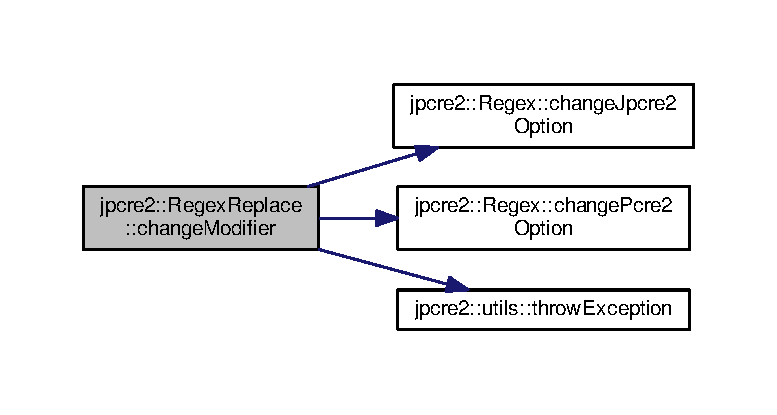
\includegraphics[width=350pt]{classjpcre2_1_1RegexReplace_ae58d2a44ed474568554202612d45c814_cgraph}
\end{center}
\end{figure}


\index{jpcre2\+::\+Regex\+Replace@{jpcre2\+::\+Regex\+Replace}!change\+Pcre2\+Option@{change\+Pcre2\+Option}}
\index{change\+Pcre2\+Option@{change\+Pcre2\+Option}!jpcre2\+::\+Regex\+Replace@{jpcre2\+::\+Regex\+Replace}}
\paragraph[{\texorpdfstring{change\+Pcre2\+Option(\+Uint opt, bool x)}{changePcre2Option(Uint opt, bool x)}}]{\setlength{\rightskip}{0pt plus 5cm}{\bf Regex\+Replace}\& jpcre2\+::\+Regex\+Replace\+::change\+Pcre2\+Option (
\begin{DoxyParamCaption}
\item[{{\bf Uint}}]{opt, }
\item[{bool}]{x}
\end{DoxyParamCaption}
)\hspace{0.3cm}{\ttfamily [inline]}}\hypertarget{classjpcre2_1_1RegexReplace_aea15c694bba7d994f048596a1f90f71f}{}\label{classjpcre2_1_1RegexReplace_aea15c694bba7d994f048596a1f90f71f}


Add or remove a P\+C\+R\+E2 option. 


\begin{DoxyParams}{Parameters}
{\em opt} & P\+C\+R\+E2 option value \\
\hline
{\em x} & Add the option if it\textquotesingle{}s true, remove otherwise. \\
\hline
\end{DoxyParams}
\begin{DoxyReturn}{Returns}
\hyperlink{classjpcre2_1_1Regex}{Regex}\& 
\end{DoxyReturn}
\begin{DoxySeeAlso}{See also}
\hyperlink{classjpcre2_1_1RegexMatch_a6893abc21b24a9d9fca146a33c0f823c}{Regex\+Match\+::change\+Pcre2\+Option()} 

\hyperlink{classjpcre2_1_1Regex_ae5bde8008cc5a700163ca3162dbd5823}{Regex\+::change\+Pcre2\+Option()} 
\end{DoxySeeAlso}
\index{jpcre2\+::\+Regex\+Replace@{jpcre2\+::\+Regex\+Replace}!replace@{replace}}
\index{replace@{replace}!jpcre2\+::\+Regex\+Replace@{jpcre2\+::\+Regex\+Replace}}
\paragraph[{\texorpdfstring{replace(void)}{replace(void)}}]{\setlength{\rightskip}{0pt plus 5cm}{\bf jpcre2\+::\+String} jpcre2\+::\+Regex\+Replace\+::replace (
\begin{DoxyParamCaption}
\item[{void}]{}
\end{DoxyParamCaption}
)}\hypertarget{classjpcre2_1_1RegexReplace_afd087fa7a9bfedec802d1a3dd7edbdd0}{}\label{classjpcre2_1_1RegexReplace_afd087fa7a9bfedec802d1a3dd7edbdd0}


Returns the resultant string after performing regex replace. 

Retrieves subject string, replacement string, modifier and other options from class variables. 
\begin{DoxyExceptions}{Exceptions}
{\em \hyperlink{classjpcre2_1_1Regex_a91b7b795c9efe76ef4e015325ff33f1c}{Regex\+::error\+\_\+number}} & Throws exception (error number) if error occurs. \\
\hline
\end{DoxyExceptions}
\begin{DoxyReturn}{Returns}
Replaced string 
\end{DoxyReturn}


References jpcre2\+::\+Regex\+::replace(), jpcre2\+::utils\+::throw\+Exception(), and jpcre2\+::utils\+::to\+String().



Referenced by jpcre2\+::\+Regex\+::replace().



Here is the call graph for this function\+:\nopagebreak
\begin{figure}[H]
\begin{center}
\leavevmode
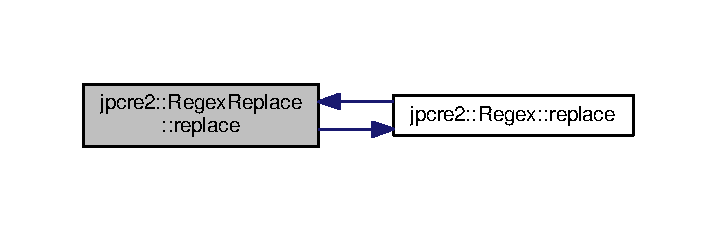
\includegraphics[width=350pt]{classjpcre2_1_1RegexReplace_afd087fa7a9bfedec802d1a3dd7edbdd0_cgraph}
\end{center}
\end{figure}




Here is the caller graph for this function\+:\nopagebreak
\begin{figure}[H]
\begin{center}
\leavevmode
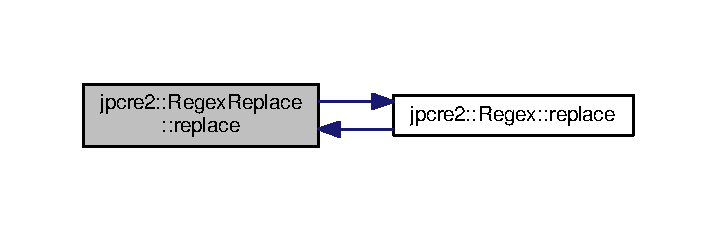
\includegraphics[width=344pt]{classjpcre2_1_1RegexReplace_afd087fa7a9bfedec802d1a3dd7edbdd0_icgraph}
\end{center}
\end{figure}


\index{jpcre2\+::\+Regex\+Replace@{jpcre2\+::\+Regex\+Replace}!set\+Buffer\+Size@{set\+Buffer\+Size}}
\index{set\+Buffer\+Size@{set\+Buffer\+Size}!jpcre2\+::\+Regex\+Replace@{jpcre2\+::\+Regex\+Replace}}
\paragraph[{\texorpdfstring{set\+Buffer\+Size(\+P\+C\+R\+E2\+\_\+\+S\+I\+Z\+E x)}{setBufferSize(PCRE2_SIZE x)}}]{\setlength{\rightskip}{0pt plus 5cm}{\bf Regex\+Replace}\& jpcre2\+::\+Regex\+Replace\+::set\+Buffer\+Size (
\begin{DoxyParamCaption}
\item[{P\+C\+R\+E2\+\_\+\+S\+I\+ZE}]{x}
\end{DoxyParamCaption}
)\hspace{0.3cm}{\ttfamily [inline]}}\hypertarget{classjpcre2_1_1RegexReplace_a452dd2632031a13b39c13b792f18a491}{}\label{classjpcre2_1_1RegexReplace_a452dd2632031a13b39c13b792f18a491}


Set the initial buffer size (\hyperlink{classjpcre2_1_1RegexReplace_a44abce541819ceb51e342411b48e95cb}{buffer\+\_\+size}) to be allocated for replaced string (used by P\+C\+R\+E2) 


\begin{DoxyParams}{Parameters}
{\em x} & Buffer size \\
\hline
\end{DoxyParams}
\begin{DoxyReturn}{Returns}
\hyperlink{classjpcre2_1_1RegexReplace}{Regex\+Replace}\& 
\end{DoxyReturn}
\index{jpcre2\+::\+Regex\+Replace@{jpcre2\+::\+Regex\+Replace}!set\+Jpcre2\+Option@{set\+Jpcre2\+Option}}
\index{set\+Jpcre2\+Option@{set\+Jpcre2\+Option}!jpcre2\+::\+Regex\+Replace@{jpcre2\+::\+Regex\+Replace}}
\paragraph[{\texorpdfstring{set\+Jpcre2\+Option(\+Uint x)}{setJpcre2Option(Uint x)}}]{\setlength{\rightskip}{0pt plus 5cm}{\bf Regex\+Replace}\& jpcre2\+::\+Regex\+Replace\+::set\+Jpcre2\+Option (
\begin{DoxyParamCaption}
\item[{{\bf Uint}}]{x}
\end{DoxyParamCaption}
)\hspace{0.3cm}{\ttfamily [inline]}}\hypertarget{classjpcre2_1_1RegexReplace_a745ab0b979035214a83ed0a04686ef6a}{}\label{classjpcre2_1_1RegexReplace_a745ab0b979035214a83ed0a04686ef6a}


Set J\+P\+C\+R\+E2 option \hyperlink{classjpcre2_1_1RegexReplace_acf13bcb16918df4b7bcaa7e49a1c7d59}{jpcre2\+\_\+replace\+\_\+opts} (overwrite existing option) 


\begin{DoxyParams}{Parameters}
{\em x} & Option value \\
\hline
\end{DoxyParams}
\begin{DoxyReturn}{Returns}
\hyperlink{classjpcre2_1_1RegexReplace}{Regex\+Replace}\& 
\end{DoxyReturn}
\begin{DoxySeeAlso}{See also}
\hyperlink{classjpcre2_1_1RegexMatch_a0d76033d9c134caa9ddfc21849603920}{Regex\+Match\+::set\+Jpcre2\+Option()} 

\hyperlink{classjpcre2_1_1Regex_a031617a19638ef752dcd2b29fa3464d5}{Regex\+::set\+Jpcre2\+Option()} 
\end{DoxySeeAlso}
\index{jpcre2\+::\+Regex\+Replace@{jpcre2\+::\+Regex\+Replace}!set\+Modifier@{set\+Modifier}}
\index{set\+Modifier@{set\+Modifier}!jpcre2\+::\+Regex\+Replace@{jpcre2\+::\+Regex\+Replace}}
\paragraph[{\texorpdfstring{set\+Modifier(const String \&s)}{setModifier(const String &s)}}]{\setlength{\rightskip}{0pt plus 5cm}{\bf Regex\+Replace}\& jpcre2\+::\+Regex\+Replace\+::set\+Modifier (
\begin{DoxyParamCaption}
\item[{const {\bf String} \&}]{s}
\end{DoxyParamCaption}
)\hspace{0.3cm}{\ttfamily [inline]}}\hypertarget{classjpcre2_1_1RegexReplace_ae2abe2994b0fbe54950f88e63000c910}{}\label{classjpcre2_1_1RegexReplace_ae2abe2994b0fbe54950f88e63000c910}


Set the modifier string (overwrites existing J\+P\+C\+R\+E2 and P\+C\+R\+E2 option). 

{\bfseries Note\+:} If speed of operation is very crucial, use \hyperlink{classjpcre2_1_1RegexReplace_a745ab0b979035214a83ed0a04686ef6a}{Regex\+Replace\+::set\+Jpcre2\+Option()} and \hyperlink{classjpcre2_1_1RegexReplace_aec36272d351fdc3a8cb02a4a3efea5a2}{Regex\+Replace\+::set\+Pcre2\+Option()} with equivalent options. It will be faster that way. 
\begin{DoxyParams}{Parameters}
{\em s} & Modifier string \\
\hline
\end{DoxyParams}
\begin{DoxyReturn}{Returns}
\hyperlink{classjpcre2_1_1RegexReplace}{Regex\+Replace}\& 
\end{DoxyReturn}
\begin{DoxySeeAlso}{See also}
\hyperlink{classjpcre2_1_1RegexMatch_a9df7e92f96b61553f62720cb8f5f23e5}{Regex\+Match\+::set\+Modifier()} 

\hyperlink{classjpcre2_1_1Regex_aed9865b58c60945e19f36fa310f5a595}{Regex\+::set\+Modifier()} 
\end{DoxySeeAlso}


Referenced by jpcre2\+::\+Regex\+::replace().



Here is the caller graph for this function\+:\nopagebreak
\begin{figure}[H]
\begin{center}
\leavevmode
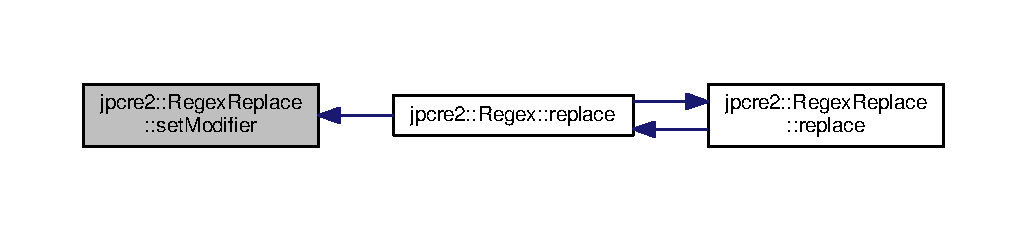
\includegraphics[width=350pt]{classjpcre2_1_1RegexReplace_ae2abe2994b0fbe54950f88e63000c910_icgraph}
\end{center}
\end{figure}


\index{jpcre2\+::\+Regex\+Replace@{jpcre2\+::\+Regex\+Replace}!set\+Pcre2\+Option@{set\+Pcre2\+Option}}
\index{set\+Pcre2\+Option@{set\+Pcre2\+Option}!jpcre2\+::\+Regex\+Replace@{jpcre2\+::\+Regex\+Replace}}
\paragraph[{\texorpdfstring{set\+Pcre2\+Option(\+Uint x)}{setPcre2Option(Uint x)}}]{\setlength{\rightskip}{0pt plus 5cm}{\bf Regex\+Replace}\& jpcre2\+::\+Regex\+Replace\+::set\+Pcre2\+Option (
\begin{DoxyParamCaption}
\item[{{\bf Uint}}]{x}
\end{DoxyParamCaption}
)\hspace{0.3cm}{\ttfamily [inline]}}\hypertarget{classjpcre2_1_1RegexReplace_aec36272d351fdc3a8cb02a4a3efea5a2}{}\label{classjpcre2_1_1RegexReplace_aec36272d351fdc3a8cb02a4a3efea5a2}


Set P\+C\+R\+E2 option \hyperlink{classjpcre2_1_1RegexReplace_afc79699cfcad8b7cbb26864b6b67cdc7}{replace\+\_\+opts} (overwrite existing option) 


\begin{DoxyParams}{Parameters}
{\em x} & Option value \\
\hline
\end{DoxyParams}
\begin{DoxyReturn}{Returns}
\hyperlink{classjpcre2_1_1RegexReplace}{Regex\+Replace}\& 
\end{DoxyReturn}
\begin{DoxySeeAlso}{See also}
\hyperlink{classjpcre2_1_1RegexMatch_ae4ab558c2bec0bc9639dbca70ab47496}{Regex\+Match\+::set\+Pcre2\+Option()} 

\hyperlink{classjpcre2_1_1Regex_acdc6f97f4030ae109c4e1a4e2310bceb}{Regex\+::set\+Pcre2\+Option()} 
\end{DoxySeeAlso}
\index{jpcre2\+::\+Regex\+Replace@{jpcre2\+::\+Regex\+Replace}!set\+Replace\+With@{set\+Replace\+With}}
\index{set\+Replace\+With@{set\+Replace\+With}!jpcre2\+::\+Regex\+Replace@{jpcre2\+::\+Regex\+Replace}}
\paragraph[{\texorpdfstring{set\+Replace\+With(const String \&s)}{setReplaceWith(const String &s)}}]{\setlength{\rightskip}{0pt plus 5cm}{\bf Regex\+Replace}\& jpcre2\+::\+Regex\+Replace\+::set\+Replace\+With (
\begin{DoxyParamCaption}
\item[{const {\bf String} \&}]{s}
\end{DoxyParamCaption}
)\hspace{0.3cm}{\ttfamily [inline]}}\hypertarget{classjpcre2_1_1RegexReplace_af1069f489de9b343493da2dc77b04c73}{}\label{classjpcre2_1_1RegexReplace_af1069f489de9b343493da2dc77b04c73}


Set the replacement string \hyperlink{classjpcre2_1_1RegexReplace_a73d0da1aac8b83a0a47b24629b5013f4}{r\+\_\+replw}. 


\begin{DoxyParams}{Parameters}
{\em s} & String to replace with \\
\hline
\end{DoxyParams}
\begin{DoxyReturn}{Returns}
\hyperlink{classjpcre2_1_1RegexReplace}{Regex\+Replace}\& 
\end{DoxyReturn}


Referenced by jpcre2\+::\+Regex\+::replace().



Here is the caller graph for this function\+:\nopagebreak
\begin{figure}[H]
\begin{center}
\leavevmode
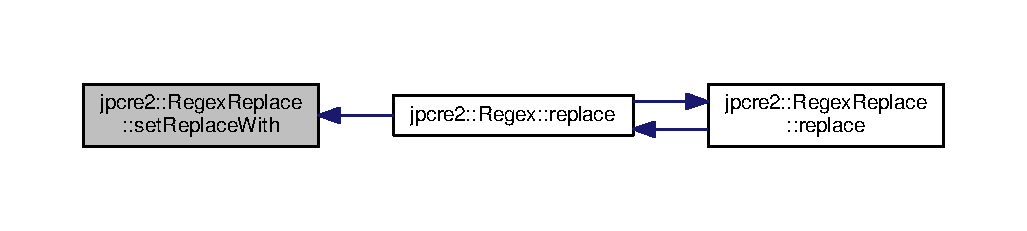
\includegraphics[width=350pt]{classjpcre2_1_1RegexReplace_af1069f489de9b343493da2dc77b04c73_icgraph}
\end{center}
\end{figure}


\index{jpcre2\+::\+Regex\+Replace@{jpcre2\+::\+Regex\+Replace}!set\+Subject@{set\+Subject}}
\index{set\+Subject@{set\+Subject}!jpcre2\+::\+Regex\+Replace@{jpcre2\+::\+Regex\+Replace}}
\paragraph[{\texorpdfstring{set\+Subject(const String \&s)}{setSubject(const String &s)}}]{\setlength{\rightskip}{0pt plus 5cm}{\bf Regex\+Replace}\& jpcre2\+::\+Regex\+Replace\+::set\+Subject (
\begin{DoxyParamCaption}
\item[{const {\bf String} \&}]{s}
\end{DoxyParamCaption}
)\hspace{0.3cm}{\ttfamily [inline]}}\hypertarget{classjpcre2_1_1RegexReplace_a46eefdb105827920bebc8436721fa4cb}{}\label{classjpcre2_1_1RegexReplace_a46eefdb105827920bebc8436721fa4cb}


Set the subject string \hyperlink{classjpcre2_1_1RegexReplace_a2290e5d9f1c2336abd431fef97e72c93}{r\+\_\+subject}. 


\begin{DoxyParams}{Parameters}
{\em s} & Subject string \\
\hline
\end{DoxyParams}
\begin{DoxyReturn}{Returns}
\hyperlink{classjpcre2_1_1RegexReplace}{Regex\+Replace}\& 
\end{DoxyReturn}
\begin{DoxySeeAlso}{See also}
\hyperlink{classjpcre2_1_1RegexMatch_a635c652195deaa8ebb9e107c4f972aab}{Regex\+Match\+::set\+Subject()} 
\end{DoxySeeAlso}


Referenced by jpcre2\+::\+Regex\+::replace().



Here is the caller graph for this function\+:\nopagebreak
\begin{figure}[H]
\begin{center}
\leavevmode
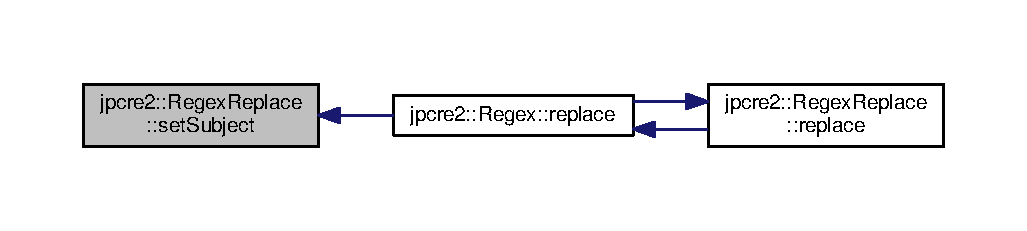
\includegraphics[width=350pt]{classjpcre2_1_1RegexReplace_a46eefdb105827920bebc8436721fa4cb_icgraph}
\end{center}
\end{figure}




The documentation for this class was generated from the following files\+:\begin{DoxyCompactItemize}
\item 
\hyperlink{jpcre2_8hpp}{jpcre2.\+hpp}\item 
jpcre2.\+cpp\end{DoxyCompactItemize}

\section{File Documentation}
\hypertarget{jpcre2_8hpp}{}\section{jpcre2.\+hpp File Reference}
\label{jpcre2_8hpp}\index{jpcre2.\+hpp@{jpcre2.\+hpp}}


Main header file for J\+P\+C\+RE library to be included by programs that call J\+P\+C\+R\+E2 functions.  


{\ttfamily \#include $<$pcre2.\+h$>$}\\*
{\ttfamily \#include $<$stdint.\+h$>$}\\*
{\ttfamily \#include $<$cstddef$>$}\\*
{\ttfamily \#include $<$string$>$}\\*
{\ttfamily \#include $<$vector$>$}\\*
{\ttfamily \#include $<$map$>$}\\*
Include dependency graph for jpcre2.\+hpp\+:\nopagebreak
\begin{figure}[H]
\begin{center}
\leavevmode
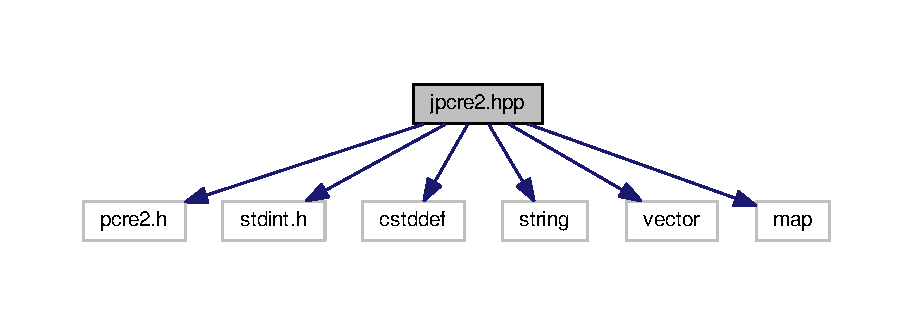
\includegraphics[width=350pt]{jpcre2_8hpp__incl}
\end{center}
\end{figure}
\subsection*{Classes}
\begin{DoxyCompactItemize}
\item 
class \hyperlink{classjpcre2_1_1RegexMatch}{jpcre2\+::\+Regex\+Match}
\begin{DoxyCompactList}\small\item\em Performs regex matching. \end{DoxyCompactList}\item 
class \hyperlink{classjpcre2_1_1RegexReplace}{jpcre2\+::\+Regex\+Replace}
\begin{DoxyCompactList}\small\item\em Performs regex replace on a string. \end{DoxyCompactList}\item 
class \hyperlink{classjpcre2_1_1Regex}{jpcre2\+::\+Regex}
\begin{DoxyCompactList}\small\item\em This is the main class that is to be used to perform all J\+P\+C\+R\+E2 related actions. \end{DoxyCompactList}\end{DoxyCompactItemize}
\subsection*{Namespaces}
\begin{DoxyCompactItemize}
\item 
 \hyperlink{namespacejpcre2}{jpcre2}
\begin{DoxyCompactList}\small\item\em Main namespace of J\+P\+C\+R\+E2. \end{DoxyCompactList}\item 
 \hyperlink{namespacejpcre2_1_1ERROR}{jpcre2\+::\+E\+R\+R\+OR}
\begin{DoxyCompactList}\small\item\em Namespace for error codes. \end{DoxyCompactList}\end{DoxyCompactItemize}
\subsection*{Macros}
\begin{DoxyCompactItemize}
\item 
\#define \hyperlink{jpcre2_8hpp_acff91275abcc225454675d6dfc39a58d}{P\+C\+R\+E2\+\_\+\+C\+O\+D\+E\+\_\+\+U\+N\+I\+T\+\_\+\+W\+I\+D\+TH}~8\hypertarget{jpcre2_8hpp_acff91275abcc225454675d6dfc39a58d}{}\label{jpcre2_8hpp_acff91275abcc225454675d6dfc39a58d}

\begin{DoxyCompactList}\small\item\em Code unit width 8 is used by default. \end{DoxyCompactList}\end{DoxyCompactItemize}
\subsection*{Typedefs}
\begin{DoxyCompactItemize}
\item 
typedef std\+::size\+\_\+t \hyperlink{namespacejpcre2_a2aac465ddcb123560c7c8215dd69246c}{jpcre2\+::\+S\+I\+Z\+E\+\_\+T}\hypertarget{namespacejpcre2_a2aac465ddcb123560c7c8215dd69246c}{}\label{namespacejpcre2_a2aac465ddcb123560c7c8215dd69246c}

\begin{DoxyCompactList}\small\item\em Used for match count and vector size. \end{DoxyCompactList}\item 
typedef uint32\+\_\+t \hyperlink{namespacejpcre2_a078242d38221a13fb3543b9edd78c099}{jpcre2\+::\+Uint}\hypertarget{namespacejpcre2_a078242d38221a13fb3543b9edd78c099}{}\label{namespacejpcre2_a078242d38221a13fb3543b9edd78c099}

\begin{DoxyCompactList}\small\item\em Used for options (bitwise operation) \end{DoxyCompactList}\item 
typedef std\+::string \hyperlink{namespacejpcre2_a91f03070152fb228bc116c5a737f1d16}{jpcre2\+::\+String}\hypertarget{namespacejpcre2_a91f03070152fb228bc116c5a737f1d16}{}\label{namespacejpcre2_a91f03070152fb228bc116c5a737f1d16}

\begin{DoxyCompactList}\small\item\em Used as std\+::string. \end{DoxyCompactList}\item 
typedef std\+::map$<$ String, String $>$ \hyperlink{namespacejpcre2_a20bd901c9ca3c949806aa6b9e324f6cf}{jpcre2\+::\+Map\+Nas}\hypertarget{namespacejpcre2_a20bd901c9ca3c949806aa6b9e324f6cf}{}\label{namespacejpcre2_a20bd901c9ca3c949806aa6b9e324f6cf}

\begin{DoxyCompactList}\small\item\em Map for Named substrings. \end{DoxyCompactList}\item 
typedef std\+::map$<$ S\+I\+Z\+E\+\_\+T, String $>$ \hyperlink{namespacejpcre2_a947e37f0e4a1678157e7f1f855638e82}{jpcre2\+::\+Map\+Num}\hypertarget{namespacejpcre2_a947e37f0e4a1678157e7f1f855638e82}{}\label{namespacejpcre2_a947e37f0e4a1678157e7f1f855638e82}

\begin{DoxyCompactList}\small\item\em Map for Numbered substrings. \end{DoxyCompactList}\item 
typedef std\+::map$<$ String, S\+I\+Z\+E\+\_\+T $>$ \hyperlink{namespacejpcre2_a753ebedfb8caf4a16ffbf47d8d705656}{jpcre2\+::\+Map\+NtN}\hypertarget{namespacejpcre2_a753ebedfb8caf4a16ffbf47d8d705656}{}\label{namespacejpcre2_a753ebedfb8caf4a16ffbf47d8d705656}

\begin{DoxyCompactList}\small\item\em Substring name to Substring number map. \end{DoxyCompactList}\item 
typedef std\+::vector$<$ Map\+Nas $>$ \hyperlink{namespacejpcre2_a2b121ae776ea5b2913839f418a7d856b}{jpcre2\+::\+Vec\+Nas}\hypertarget{namespacejpcre2_a2b121ae776ea5b2913839f418a7d856b}{}\label{namespacejpcre2_a2b121ae776ea5b2913839f418a7d856b}

\begin{DoxyCompactList}\small\item\em Vector of matches with named substrings. \end{DoxyCompactList}\item 
typedef std\+::vector$<$ Map\+NtN $>$ \hyperlink{namespacejpcre2_a88a7aaf84cad627d34c8152e726168eb}{jpcre2\+::\+Vec\+NtN}\hypertarget{namespacejpcre2_a88a7aaf84cad627d34c8152e726168eb}{}\label{namespacejpcre2_a88a7aaf84cad627d34c8152e726168eb}

\begin{DoxyCompactList}\small\item\em Vector of substring name to Substring number map. \end{DoxyCompactList}\item 
typedef std\+::vector$<$ Map\+Num $>$ \hyperlink{namespacejpcre2_ac1cf752c8fbb0be78020be3b80e77ce3}{jpcre2\+::\+Vec\+Num}\hypertarget{namespacejpcre2_ac1cf752c8fbb0be78020be3b80e77ce3}{}\label{namespacejpcre2_ac1cf752c8fbb0be78020be3b80e77ce3}

\begin{DoxyCompactList}\small\item\em Vector of matches with numbered substrings. \end{DoxyCompactList}\end{DoxyCompactItemize}
\subsection*{Enumerations}
\subsection*{Functions}
\begin{DoxyCompactItemize}
\item 
String \hyperlink{jpcre2_8hpp_a433f24d37008ed65f829be30aa0f2c73}{jpcre2\+::utils\+::to\+String} (int a)\hypertarget{jpcre2_8hpp_a433f24d37008ed65f829be30aa0f2c73}{}\label{jpcre2_8hpp_a433f24d37008ed65f829be30aa0f2c73}

\begin{DoxyCompactList}\small\item\em Converts an integer to String. \end{DoxyCompactList}\item 
String \hyperlink{jpcre2_8hpp_a8951a9c2c01a87cee04b55d0a032c73e}{jpcre2\+::utils\+::to\+String} (char a)\hypertarget{jpcre2_8hpp_a8951a9c2c01a87cee04b55d0a032c73e}{}\label{jpcre2_8hpp_a8951a9c2c01a87cee04b55d0a032c73e}

\begin{DoxyCompactList}\small\item\em Converts a char to String. \end{DoxyCompactList}\item 
String \hyperlink{jpcre2_8hpp_a67c67163e03c18ca3418f5f59f90b435}{jpcre2\+::utils\+::to\+String} (const char $\ast$a)\hypertarget{jpcre2_8hpp_a67c67163e03c18ca3418f5f59f90b435}{}\label{jpcre2_8hpp_a67c67163e03c18ca3418f5f59f90b435}

\begin{DoxyCompactList}\small\item\em Converts const char$\ast$ to String. \end{DoxyCompactList}\item 
String \hyperlink{jpcre2_8hpp_a84c5c4e28feda8b093d700a911d59c72}{jpcre2\+::utils\+::to\+String} (P\+C\+R\+E2\+\_\+\+U\+C\+H\+AR $\ast$a)\hypertarget{jpcre2_8hpp_a84c5c4e28feda8b093d700a911d59c72}{}\label{jpcre2_8hpp_a84c5c4e28feda8b093d700a911d59c72}

\begin{DoxyCompactList}\small\item\em Converts a P\+C\+R\+E2\+\_\+\+U\+C\+H\+A\+R$\ast$ to String. \end{DoxyCompactList}\item 
String \hyperlink{jpcre2_8hpp_a186305c70ad9dc4137aae2bcbf644805}{jpcre2\+::utils\+::get\+Pcre2\+Error\+Message} (int err\+\_\+num)\hypertarget{jpcre2_8hpp_a186305c70ad9dc4137aae2bcbf644805}{}\label{jpcre2_8hpp_a186305c70ad9dc4137aae2bcbf644805}

\begin{DoxyCompactList}\small\item\em Get P\+C\+R\+E2 error message for an error number. \end{DoxyCompactList}\end{DoxyCompactItemize}
\subsection*{Variables}
\begin{DoxyCompactItemize}
\item 
const S\+I\+Z\+E\+\_\+T \hyperlink{namespacejpcre2_a80cb201f2e733137b22a8ed98465096a}{jpcre2\+::\+S\+U\+B\+S\+T\+I\+T\+U\+T\+E\+\_\+\+R\+E\+S\+U\+L\+T\+\_\+\+I\+N\+I\+T\+\_\+\+S\+I\+ZE} = std\+::numeric\+\_\+limits$<$int$>$\+::max()
\begin{DoxyCompactList}\small\item\em Used by default to provide big enough buffer for replaced string. \end{DoxyCompactList}\item 
const String \hyperlink{namespacejpcre2_ad2236dcdcc14d580724b256ce7f168e5}{jpcre2\+::\+L\+O\+C\+A\+L\+E\+\_\+\+N\+O\+NE} = \char`\"{}J\+P\+C\+R\+E2\+\_\+\+N\+O\+NE\char`\"{}
\begin{DoxyCompactList}\small\item\em Don\textquotesingle{}t do anything about locale if it is set to L\+O\+C\+A\+L\+E\+\_\+\+N\+O\+NE. \end{DoxyCompactList}\item 
const String \hyperlink{namespacejpcre2_adfdd3d1fff99e685734ae4e59771e84d}{jpcre2\+::\+L\+O\+C\+A\+L\+E\+\_\+\+D\+E\+F\+A\+U\+LT} = L\+O\+C\+A\+L\+E\+\_\+\+N\+O\+NE
\begin{DoxyCompactList}\small\item\em Default locale. \end{DoxyCompactList}\item 
const String \hyperlink{namespacejpcre2_abf6c3bff9268a572c299958d334ff26e}{jpcre2\+::\+J\+I\+T\+\_\+\+E\+R\+R\+O\+R\+\_\+\+M\+E\+S\+S\+A\+G\+E\+\_\+\+P\+R\+E\+F\+IX} = \char`\"{}J\+IT compilation failed! \char`\"{}\hypertarget{namespacejpcre2_abf6c3bff9268a572c299958d334ff26e}{}\label{namespacejpcre2_abf6c3bff9268a572c299958d334ff26e}

\begin{DoxyCompactList}\small\item\em Prefix to be added to J\+IT error message. \end{DoxyCompactList}\end{DoxyCompactItemize}


\subsection{Detailed Description}
Main header file for J\+P\+C\+RE library to be included by programs that call J\+P\+C\+R\+E2 functions. 

It includes the pcre2.\+h header, therefore you shouldn\textquotesingle{}t include pcre2.\+h separately in your program. Make sure to link pcre2 library when compiling. If you are using J\+P\+C\+R\+E2 as a library, then link this library too. \begin{DoxyAuthor}{Author}
Md. Jahidul Hamid. 
\end{DoxyAuthor}

\hypertarget{test__match_8cpp}{}\subsection{test\+\_\+match.\+cpp File Reference}
\label{test__match_8cpp}\index{test\+\_\+match.\+cpp@{test\+\_\+match.\+cpp}}


An example of performing regex match against a pattern with J\+P\+C\+R\+E2 and getting the match count and match results.  


{\ttfamily \#include $<$iostream$>$}\\*
{\ttfamily \#include \char`\"{}jpcre2.\+hpp\char`\"{}}\\*
Include dependency graph for test\+\_\+match.\+cpp\+:\nopagebreak
\begin{figure}[H]
\begin{center}
\leavevmode
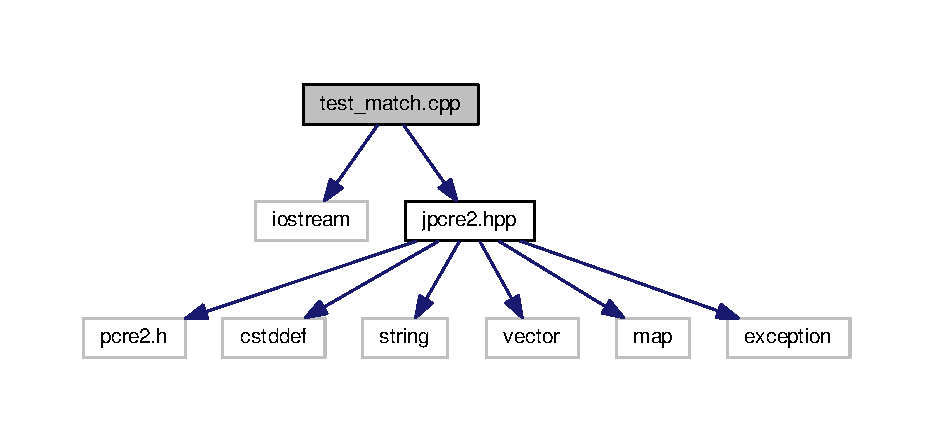
\includegraphics[width=350pt]{test__match_8cpp__incl}
\end{center}
\end{figure}


\subsubsection{Detailed Description}
An example of performing regex match against a pattern with J\+P\+C\+R\+E2 and getting the match count and match results. 

Shows how to iterate over the match results to get the captured groups/substrings. 
\begin{DoxyCodeInclude}
\textcolor{comment}{/**@file test\_match.cpp}
\textcolor{comment}{ * An example of performing regex match against a pattern with JPCRE2 and getting the}
\textcolor{comment}{ * match count and match results.}
\textcolor{comment}{ * Shows how to iterate over the match results to get the captured groups/substrings.}
\textcolor{comment}{ * @include test\_match.cpp}
\textcolor{comment}{ * @author [Md Jahidul Hamid](https://github.com/neurobin)}
\textcolor{comment}{ * */}

\textcolor{preprocessor}{#include <iostream>}
\textcolor{preprocessor}{#include "\hyperlink{jpcre2_8hpp}{jpcre2.hpp}"}


\textcolor{keywordtype}{int} main()\{

    \hyperlink{namespacejpcre2_ac1cf752c8fbb0be78020be3b80e77ce3}{jpcre2::VecNum} vec\_num0;   \textcolor{comment}{///Vector to store numbered substring Maps.}
\textcolor{comment}{}    \hyperlink{namespacejpcre2_a2b121ae776ea5b2913839f418a7d856b}{jpcre2::VecNas} vec\_nas0;   \textcolor{comment}{///Vector to store named substring Maps.}
\textcolor{comment}{}    \hyperlink{namespacejpcre2_a88a7aaf84cad627d34c8152e726168eb}{jpcre2::VecNtN} vec\_nn0;    \textcolor{comment}{///Vector to store Named substring to Number Maps.}
\textcolor{comment}{}    
    \hyperlink{classjpcre2_1_1Regex}{jpcre2::Regex} re;     \textcolor{comment}{///It's not supposed to throw any exception.}
\textcolor{comment}{}    \textcolor{comment}{}
\textcolor{comment}{    ///Compile the pattern}
\textcolor{comment}{}    \textcolor{keywordflow}{try}\{re.\hyperlink{classjpcre2_1_1Regex_a85d9a514ea86ae68533223adac6c6bd8}{setPattern}(\textcolor{stringliteral}{"(?:(?<word>[?.#@:]+)|(?<word>\(\backslash\)\(\backslash\)w+))\(\backslash\)\(\backslash\)s*(?<digit>\(\backslash\)\(\backslash\)d+)"})  \textcolor{comment}{//set pattern}
          .\hyperlink{classjpcre2_1_1Regex_aed9865b58c60945e19f36fa310f5a595}{setModifier}(\textcolor{stringliteral}{"nJ"})                                                    \textcolor{comment}{//set modifier}
          .\hyperlink{classjpcre2_1_1Regex_a03974fa7ba8f7c47186cb8d6f54934de}{addJpcre2Option}(\hyperlink{namespacejpcre2_a85c143271501e383843f45b9999c2f00a9124b768bcae4d51430aa7f26126f387}{jpcre2::VALIDATE\_MODIFIER}               
                   \textcolor{comment}{//modifier goes through validation check}
                            | \hyperlink{namespacejpcre2_a85c143271501e383843f45b9999c2f00a5e8bab7c478015b19baf3e84ed00876e}{jpcre2::JIT\_COMPILE}                               \textcolor{comment}{//
      perform JIT compile (warning if JIT is not available)}
                            | \hyperlink{namespacejpcre2_a85c143271501e383843f45b9999c2f00a6fec35fc9fdd8a606bed430c1816c552}{jpcre2::ERROR\_ALL})                                \textcolor{comment}{//treat
       warnings as errors}
          .\hyperlink{classjpcre2_1_1Regex_a2c7dcf12f26b2b046e147b013c8b5087}{addPcre2Option}(0)                                                    \textcolor{comment}{//add pcre2
       option}
          .\hyperlink{classjpcre2_1_1Regex_aad1d5ef1e87f762f68a587eec4022e69}{compile}();\}                                                          \textcolor{comment}{//Finally compile
       it.}
    \textcolor{keywordflow}{catch}(\textcolor{keywordtype}{int} e)\{std::cerr<<re.\hyperlink{classjpcre2_1_1Regex_a92b75c438ccff871205b2175a6141fd5}{getErrorMessage}(e);\}
    \textcolor{comment}{}
\textcolor{comment}{    /// The above `jpcre2::VALIDATE\_MODIFIER` option won't have any effect as modifier was passe before it.}
\textcolor{comment}{    /// You can pass a modifier (~ or &) to turn this validation check on. In that case}
\textcolor{comment}{    /// validation will start after ~ or & modifier is encountered,}
\textcolor{comment}{}
    \textcolor{comment}{/******************************************************************************************************
      *********}
\textcolor{comment}{     * Always use try catch to catch any exception and avoid unexpected termination of the program.}
\textcolor{comment}{     * All jpcre2 exceptions are of type int (integer)}
\textcolor{comment}{     * ****************************************************************************************************
      *********/}
    \textcolor{comment}{}
\textcolor{comment}{    ///subject string}
\textcolor{comment}{}    std::string subject = \textcolor{stringliteral}{"(I am a string with words and digits 45 and specials chars: ?.#@ 443 অ আ ক খ গ ঘ
        56)"};
    
    \textcolor{keywordtype}{size\_t} count=0;
    
    \textcolor{keywordflow}{try}\{count = re.\hyperlink{classjpcre2_1_1Regex_a519b0915bf1163c6ce6a4d674b30cfcd}{initMatch}()                                  \textcolor{comment}{//Invoke the initMatch() function}
                  .\hyperlink{classjpcre2_1_1RegexMatch_a9df7e92f96b61553f62720cb8f5f23e5}{setModifier}(\textcolor{stringliteral}{"gf"})                            \textcolor{comment}{//set various parameters (f:
       invalid modifier)}
                  .\hyperlink{classjpcre2_1_1RegexMatch_a635c652195deaa8ebb9e107c4f972aab}{setSubject}(subject)                          \textcolor{comment}{//...}
                  .\hyperlink{classjpcre2_1_1RegexMatch_a2c7efe1ec2e13827f670db4ecedcd0a0}{setNumberedSubstringVector}(&vec\_num0)        \textcolor{comment}{//...}
                  .\hyperlink{classjpcre2_1_1RegexMatch_ae495431f57cae54363331237ab21b56c}{setNamedSubstringVector}(&vec\_nas0)           \textcolor{comment}{//...}
                  .\hyperlink{classjpcre2_1_1RegexMatch_a04926e61d8b5f1d8bdf344efecd567d8}{setNameToNumberMapVector}(&vec\_nn0)           \textcolor{comment}{//...}
                  .\hyperlink{classjpcre2_1_1RegexMatch_a0a4cf8554a7e00f3cf2db34f60a43f60}{addJpcre2Option}(\hyperlink{namespacejpcre2_a85c143271501e383843f45b9999c2f00a9124b768bcae4d51430aa7f26126f387}{jpcre2::VALIDATE\_MODIFIER})   \textcolor{comment}{//
      ...}
                  .\hyperlink{classjpcre2_1_1RegexMatch_aac4857cd8f5eae15b29b9afbe9023522}{addPcre2Option}(0)                            \textcolor{comment}{//...}
                  .\hyperlink{classjpcre2_1_1RegexMatch_a5868aef3a146594ea1ebef34d122bb33}{match}();\}                                    \textcolor{comment}{//Finally perform the match}
    \textcolor{keywordflow}{catch}(\textcolor{keywordtype}{int} e)\{std::cerr<<\textcolor{stringliteral}{"\(\backslash\)n"}<<re.\hyperlink{classjpcre2_1_1Regex_a92b75c438ccff871205b2175a6141fd5}{getErrorMessage}(e);\}
    
    std::cerr<<re.\hyperlink{classjpcre2_1_1Regex_a1a639ae4090b88609c03e9268faf02d8}{getWarningMessage}(); \textcolor{comment}{//(f: invalid modifier) warning}
    \textcolor{comment}{}
\textcolor{comment}{    /// re.reset(); /// re-initialize re}
\textcolor{comment}{}    
    
    std::cout<<\textcolor{stringliteral}{"\(\backslash\)nTotal number of mathces: "}<<count<<std::endl;\textcolor{comment}{}
\textcolor{comment}{    ///Now let's access the matched data}
\textcolor{comment}{}    \textcolor{comment}{}
\textcolor{comment}{    ///Each of these vectors contains maps.}
\textcolor{comment}{    ///Each element in the vector specifies a particular match}
\textcolor{comment}{    ///First match is the vector element 0, second is at index 1 and so forth}
\textcolor{comment}{    ///A map for a vector element, i.e for a match contains all of its substrings/capture groups}
\textcolor{comment}{    ///The first element of the map is capture group 0 i.e total match}
\textcolor{comment}{}    
    
    \textcolor{keywordflow}{for}(\textcolor{keywordtype}{size\_t} i=0;i<vec\_num0.size();++i)\{
        
        
        std::cout<< \textcolor{stringliteral}{"\(\backslash\)n################## Match no: "}<<i+1<<\textcolor{stringliteral}{" ####################\(\backslash\)n"};
        
        
        \textcolor{comment}{}
\textcolor{comment}{        ///This vector contains maps with number as the key and the corresponding substring as the value}
\textcolor{comment}{}        std::cout<<\textcolor{stringliteral}{"\(\backslash\)n-------------------------------------------------------------------------"};
        std::cout<< \textcolor{stringliteral}{"\(\backslash\)n--- Numbered Substrings (number: substring) for match "}<<i+1<<\textcolor{stringliteral}{" ---\(\backslash\)n"};
        \textcolor{keywordflow}{for}(jpcre2::MapNum::iterator ent=vec\_num0[i].begin();ent!=vec\_num0[i].end();++ent)\{
            std::cout<<\textcolor{stringliteral}{"\(\backslash\)n\(\backslash\)t"}<<ent->first<<\textcolor{stringliteral}{": "}<<ent->second<<\textcolor{stringliteral}{"\(\backslash\)n"};
        \}
        
        
        \textcolor{comment}{}
\textcolor{comment}{        ///This vector contains maps with name as the key and the corresponding substring as the value}
\textcolor{comment}{}        std::cout<<\textcolor{stringliteral}{"\(\backslash\)n-------------------------------------------------------------------------"};
        std::cout<< \textcolor{stringliteral}{"\(\backslash\)n--- Named Substrings (name: substring) for match "}<<i+1<<\textcolor{stringliteral}{" ---\(\backslash\)n"};
        \textcolor{keywordflow}{for}(jpcre2::MapNas::iterator ent=vec\_nas0[i].begin();ent!=vec\_nas0[i].end();++ent)\{
            std::cout<<\textcolor{stringliteral}{"\(\backslash\)n\(\backslash\)t"}<<ent->first<<\textcolor{stringliteral}{": "}<<ent->second<<\textcolor{stringliteral}{"\(\backslash\)n"};
        \}
        
        
        \textcolor{comment}{}
\textcolor{comment}{        ///This vector contains maps with name as the key and number as the value}
\textcolor{comment}{        ///i.e the number (of substring) can be accessed with the name for named substring.}
\textcolor{comment}{}        std::cout<<\textcolor{stringliteral}{"\(\backslash\)n-------------------------------------------------------------------------"};
        std::cout<< \textcolor{stringliteral}{"\(\backslash\)n--- Name to number mapping (name: number/position) for match "}<<i+1<<\textcolor{stringliteral}{" ---\(\backslash\)n"};
        \textcolor{keywordflow}{for}(jpcre2::MapNtN::iterator ent=vec\_nn0[i].begin();ent!=vec\_nn0[i].end();++ent)\{
            std::cout<<\textcolor{stringliteral}{"\(\backslash\)n\(\backslash\)t"}<<ent->first<<\textcolor{stringliteral}{": "}<<ent->second<<\textcolor{stringliteral}{"\(\backslash\)n"};
        \}
    \}
    \textcolor{keywordflow}{return} 0;
\}
\end{DoxyCodeInclude}
 \begin{DoxyAuthor}{Author}
\href{https://github.com/neurobin}{\tt Md Jahidul Hamid} 
\end{DoxyAuthor}

\hypertarget{test__match2_8cpp}{}\section{test\+\_\+match2.\+cpp File Reference}
\label{test__match2_8cpp}\index{test\+\_\+match2.\+cpp@{test\+\_\+match2.\+cpp}}
{\ttfamily \#include $<$iostream$>$}\\*
{\ttfamily \#include \char`\"{}jpcre2.\+hpp\char`\"{}}\\*
\subsection*{Macros}
\begin{DoxyCompactItemize}
\item 
\#define \hyperlink{test__match2_8cpp_a0efdcb15269092623bd8d80b8d129239}{get\+Line}(a)~std\+::getline(std\+::cin,a,\textquotesingle{}\textbackslash{}n\textquotesingle{});
\end{DoxyCompactItemize}
\subsection*{Functions}
\begin{DoxyCompactItemize}
\item 
int \hyperlink{test__match2_8cpp_ae66f6b31b5ad750f1fe042a706a4e3d4}{main} ()
\end{DoxyCompactItemize}


\subsection{Macro Definition Documentation}
\index{test\+\_\+match2.\+cpp@{test\+\_\+match2.\+cpp}!get\+Line@{get\+Line}}
\index{get\+Line@{get\+Line}!test\+\_\+match2.\+cpp@{test\+\_\+match2.\+cpp}}
\subsubsection[{\texorpdfstring{get\+Line}{getLine}}]{\setlength{\rightskip}{0pt plus 5cm}\#define get\+Line(
\begin{DoxyParamCaption}
\item[{}]{a}
\end{DoxyParamCaption}
)~std\+::getline(std\+::cin,a,\textquotesingle{}\textbackslash{}n\textquotesingle{});}\hypertarget{test__match2_8cpp_a0efdcb15269092623bd8d80b8d129239}{}\label{test__match2_8cpp_a0efdcb15269092623bd8d80b8d129239}


\subsection{Function Documentation}
\index{test\+\_\+match2.\+cpp@{test\+\_\+match2.\+cpp}!main@{main}}
\index{main@{main}!test\+\_\+match2.\+cpp@{test\+\_\+match2.\+cpp}}
\subsubsection[{\texorpdfstring{main()}{main()}}]{\setlength{\rightskip}{0pt plus 5cm}int main (
\begin{DoxyParamCaption}
{}
\end{DoxyParamCaption}
)}\hypertarget{test__match2_8cpp_ae66f6b31b5ad750f1fe042a706a4e3d4}{}\label{test__match2_8cpp_ae66f6b31b5ad750f1fe042a706a4e3d4}
Vector to store numbured substring Map.

Vector to store named substring Map.

Vector to store Named substring to Number Map.

create an object

This should not throw any exception

Compile pattern

subject string

Now let\textquotesingle{}s access the matched data

Each of these vectors contains a map and each of the maps contains all the substrings that are matched against the pattern. All the matches in all the maps combines the total match throughout the entire string.

This vector contains maps with number as the key and the corresponding substring as the value

This vector contains maps with name as the key and the corresponding substring as the value

This vector contains maps with name as the key and number as the value i.\+e the number (of substring) can be accessed with the name for named substring. 
\hypertarget{test__replace_8cpp}{}\subsection{test\+\_\+replace.\+cpp File Reference}
\label{test__replace_8cpp}\index{test\+\_\+replace.\+cpp@{test\+\_\+replace.\+cpp}}


An example of doing regex replace with J\+P\+C\+R\+E2.  


{\ttfamily \#include $<$iostream$>$}\\*
{\ttfamily \#include \char`\"{}jpcre2.\+hpp\char`\"{}}\\*
Include dependency graph for test\+\_\+replace.\+cpp\+:\nopagebreak
\begin{figure}[H]
\begin{center}
\leavevmode
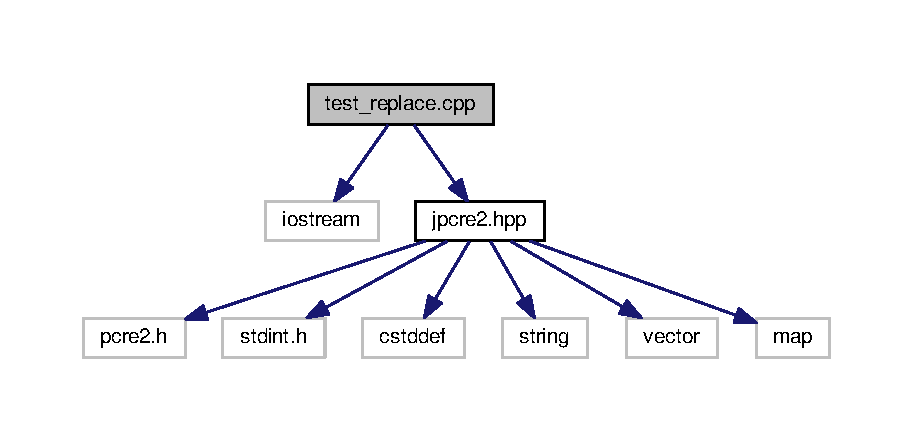
\includegraphics[width=350pt]{test__replace_8cpp__incl}
\end{center}
\end{figure}


\subsubsection{Detailed Description}
An example of doing regex replace with J\+P\+C\+R\+E2. 


\begin{DoxyCodeInclude}
\textcolor{comment}{/**@file test\_replace.cpp}
\textcolor{comment}{ * An example of doing regex replace with JPCRE2}
\textcolor{comment}{ * @include test\_replace.cpp}
\textcolor{comment}{ * @author [Md Jahidul Hamid](https://github.com/neurobin)}
\textcolor{comment}{ * */}

\textcolor{preprocessor}{#include <iostream>}
\textcolor{preprocessor}{#include "\hyperlink{jpcre2_8hpp}{jpcre2.hpp}"}


\textcolor{keywordtype}{int} main()\{
    \hyperlink{classjpcre2_1_1Regex}{jpcre2::Regex} re;     \textcolor{comment}{/// This is not supposed to throw any exception.}
\textcolor{comment}{}\textcolor{comment}{}
\textcolor{comment}{    ///Compile the pattern}
\textcolor{comment}{}    \textcolor{keywordflow}{try}\{re.\hyperlink{classjpcre2_1_1Regex_a85d9a514ea86ae68533223adac6c6bd8}{setPattern}(\textcolor{stringliteral}{"(?:(?<word>[?.#@:]+)|(?<word>\(\backslash\)\(\backslash\)w+))\(\backslash\)\(\backslash\)s*(?<digit>\(\backslash\)\(\backslash\)d+)"})     \textcolor{comment}{//Set various
       parameters}
          .\hyperlink{classjpcre2_1_1Regex_aed9865b58c60945e19f36fa310f5a595}{setModifier}(\textcolor{stringliteral}{"Jin"})                                                      \textcolor{comment}{//...}
          .\hyperlink{classjpcre2_1_1Regex_a03974fa7ba8f7c47186cb8d6f54934de}{addJpcre2Option}(\hyperlink{namespacejpcre2_a85c143271501e383843f45b9999c2f00a9124b768bcae4d51430aa7f26126f387}{jpcre2::VALIDATE\_MODIFIER})              
                      \textcolor{comment}{//...}
          .\hyperlink{classjpcre2_1_1Regex_a2c7dcf12f26b2b046e147b013c8b5087}{addPcre2Option}(0)                                                       \textcolor{comment}{//...}
          .\hyperlink{classjpcre2_1_1Regex_aad1d5ef1e87f762f68a587eec4022e69}{compile}();\}                                                             \textcolor{comment}{//Finally compile
       it.}
    \textcolor{keywordflow}{catch}(\textcolor{keywordtype}{int} e)\{std::cerr<<re.\hyperlink{classjpcre2_1_1Regex_a92b75c438ccff871205b2175a6141fd5}{getErrorMessage}(e);\}
        
    \textcolor{comment}{/******************************************************************************************************
      ************}
\textcolor{comment}{     * Use try catch block to catch any exception and avoid unexpected termination of the program in case
       of error}
\textcolor{comment}{     * All jpcre2 exceptions are of type int (integer)}
\textcolor{comment}{     * ****************************************************************************************************
      ************/}
    
    \textcolor{comment}{//subject string}
    std::string s=\textcolor{stringliteral}{"I am a string with words and digits 45 and specials chars: ?.#@ 443 অ আ ক খ গ ঘ  56"};
    
    \textcolor{keywordflow}{try}\{std::cout<<\textcolor{stringliteral}{"\(\backslash\)nreplaced string: \(\backslash\)n"}<<
        re.\hyperlink{classjpcre2_1_1Regex_ae7235a991492fa88f1bd3fb02d59cd0a}{initReplace}()                                                    \textcolor{comment}{//Invoke the
       initReplace() function}
          .\hyperlink{classjpcre2_1_1RegexReplace_a46eefdb105827920bebc8436721fa4cb}{setSubject}(s)                                                    \textcolor{comment}{//Set various
       parameters}
          .\hyperlink{classjpcre2_1_1RegexReplace_af1069f489de9b343493da2dc77b04c73}{setReplaceWith}(\textcolor{stringliteral}{"(replaced:$1)(replaced:$2)(replaced:$\{word\})"})   \textcolor{comment}{//...}
          .\hyperlink{classjpcre2_1_1RegexReplace_ae2abe2994b0fbe54950f88e63000c910}{setModifier}(\textcolor{stringliteral}{"xE"})                                                \textcolor{comment}{//...}
          .\hyperlink{classjpcre2_1_1RegexReplace_a3f86b1e11d08d0153a08244771e59061}{addJpcre2Option}(\hyperlink{namespacejpcre2_a85c143271501e383843f45b9999c2f00a9124b768bcae4d51430aa7f26126f387}{jpcre2::VALIDATE\_MODIFIER})              
               \textcolor{comment}{//...}
          .\hyperlink{classjpcre2_1_1RegexReplace_a3cfd03568b23bebcbb530a2c120b5d33}{addPcre2Option}(0)                                                \textcolor{comment}{//...}
          .\hyperlink{classjpcre2_1_1RegexReplace_afd087fa7a9bfedec802d1a3dd7edbdd0}{replace}();                                                       \textcolor{comment}{//Finally perform the
       replace operation.}
    \}
    \textcolor{keywordflow}{catch}(\textcolor{keywordtype}{int} e)\{std::cerr<<re.\hyperlink{classjpcre2_1_1Regex_a92b75c438ccff871205b2175a6141fd5}{getErrorMessage}(e);\}
    
    \textcolor{keywordflow}{return} 0;
\}
\end{DoxyCodeInclude}
 \begin{DoxyAuthor}{Author}
\href{https://github.com/neurobin}{\tt Md Jahidul Hamid} 
\end{DoxyAuthor}

\hypertarget{test__replace2_8cpp}{}\subsection{test\+\_\+replace2.\+cpp File Reference}
\label{test__replace2_8cpp}\index{test\+\_\+replace2.\+cpp@{test\+\_\+replace2.\+cpp}}


Contains an example to take subject string, replacement string, modifier and pattern from user input and perform regex replace with J\+P\+C\+R\+E2.  


{\ttfamily \#include $<$iostream$>$}\\*
{\ttfamily \#include \char`\"{}jpcre2.\+hpp\char`\"{}}\\*
Include dependency graph for test\+\_\+replace2.\+cpp\+:\nopagebreak
\begin{figure}[H]
\begin{center}
\leavevmode
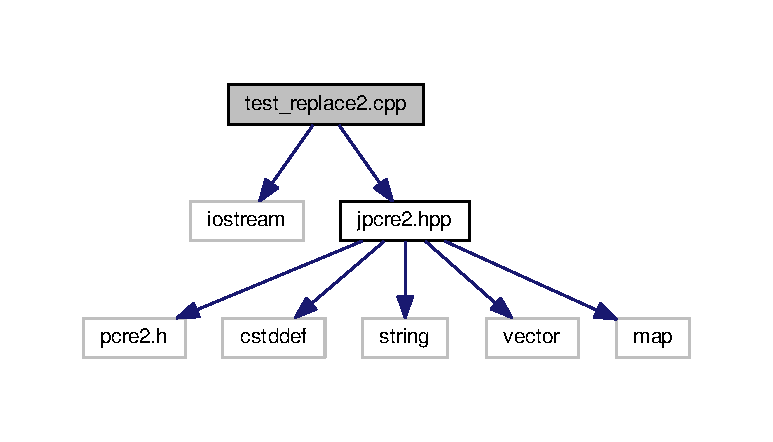
\includegraphics[width=350pt]{test__replace2_8cpp__incl}
\end{center}
\end{figure}


\subsubsection{Detailed Description}
Contains an example to take subject string, replacement string, modifier and pattern from user input and perform regex replace with J\+P\+C\+R\+E2. 


\begin{DoxyCodeInclude}
\textcolor{comment}{/**@file test\_replace2.cpp}
\textcolor{comment}{ * Contains an example to take subject string, replacement string, modifier and pattern}
\textcolor{comment}{ * from user input and perform regex replace with JPCRE2}
\textcolor{comment}{ * @include test\_replace2.cpp}
\textcolor{comment}{ * @author [Md Jahidul Hamid](https://github.com/neurobin)}
\textcolor{comment}{ * */}


\textcolor{preprocessor}{#include <iostream>}
\textcolor{preprocessor}{#include "\hyperlink{jpcre2_8hpp}{jpcre2.hpp}"}


\textcolor{preprocessor}{#define getLine(a) std::getline(std::cin,a,'\(\backslash\)n')}


\textcolor{keywordtype}{int} main()\{
    std::string pat,mod,subject,repl,repl\_mod;

    std::cout<<\textcolor{stringliteral}{"\(\backslash\)nEnter pattern: "};
    getLine(pat);

    std::cout<<\textcolor{stringliteral}{"\(\backslash\)nEnter compile modifiers (eijmnsuxADJSU): "};
    getLine(mod);
    \hyperlink{classjpcre2_1_1Regex}{jpcre2::Regex} re;     \textcolor{comment}{/// This is not supposed to throw any exception.}
\textcolor{comment}{}
\textcolor{comment}{}
\textcolor{comment}{    /// Compile the pattern}
\textcolor{comment}{}    \textcolor{keywordflow}{try}\{re.\hyperlink{classjpcre2_1_1Regex_aad1d5ef1e87f762f68a587eec4022e69}{compile}(pat,mod);\}
    \textcolor{keywordflow}{catch}(\textcolor{keywordtype}{int} e)\{std::cerr<<re.\hyperlink{classjpcre2_1_1Regex_a92b75c438ccff871205b2175a6141fd5}{getErrorMessage}(e);\}


    \textcolor{comment}{/******************************************************************************************************
      *********}
\textcolor{comment}{     * Use try catch block to catch any exception and avoid unexpected termination of the program in case
       of error.}
\textcolor{comment}{     * All jpcre2 exceptions are of type int (integer)}
\textcolor{comment}{     * ****************************************************************************************************
      *********/}

\textcolor{comment}{}
\textcolor{comment}{    ///subject string}
\textcolor{comment}{}    std::cout<<\textcolor{stringliteral}{"\(\backslash\)nEnter subject string (enter quit to quit): "}<<std::endl;
    getLine(subject);
    \textcolor{keywordflow}{if}(subject==\textcolor{stringliteral}{"quit"})\textcolor{keywordflow}{return} 0;\textcolor{comment}{}
\textcolor{comment}{     ///replacement string}
\textcolor{comment}{}    std::cout<<\textcolor{stringliteral}{"\(\backslash\)nEnter replacement string: "}<<std::endl;
    getLine(repl);
\textcolor{comment}{}
\textcolor{comment}{    /// Continue loop as long as error occurs}
\textcolor{comment}{}    \textcolor{keywordflow}{while}(\textcolor{keyword}{true})\{
        std::cout<<\textcolor{stringliteral}{"\(\backslash\)nEnter action (replacement) modifiers (eEgx): "};
        getLine(repl\_mod);

        \textcolor{comment}{//perform replace}

        \textcolor{keywordflow}{try}\{std::cout<<\textcolor{stringliteral}{"\(\backslash\)nreplaced string: "}<<re.\hyperlink{classjpcre2_1_1Regex_ae7235a991492fa88f1bd3fb02d59cd0a}{initReplace}()
                                                .\hyperlink{classjpcre2_1_1RegexReplace_a46eefdb105827920bebc8436721fa4cb}{setSubject}(subject)
                                                .\hyperlink{classjpcre2_1_1RegexReplace_af1069f489de9b343493da2dc77b04c73}{setReplaceWith}(repl)
                                                .\hyperlink{classjpcre2_1_1RegexReplace_a3f86b1e11d08d0153a08244771e59061}{addJpcre2Option}(
      \hyperlink{namespacejpcre2_a85c143271501e383843f45b9999c2f00a9124b768bcae4d51430aa7f26126f387}{jpcre2::VALIDATE\_MODIFIER})
                                                .\hyperlink{classjpcre2_1_1RegexReplace_a06a57430f62058822d48722a2a6425d7}{addModifier}(repl\_mod)
                                                .\hyperlink{classjpcre2_1_1RegexReplace_afd087fa7a9bfedec802d1a3dd7edbdd0}{replace}();\}
        \textcolor{keywordflow}{catch}(\textcolor{keywordtype}{int} e)\{std::cerr<<re.\hyperlink{classjpcre2_1_1Regex_a92b75c438ccff871205b2175a6141fd5}{getErrorMessage}(e);
            \textcolor{keywordflow}{if}(e==\hyperlink{namespacejpcre2_1_1ERROR_a4b2998984439438fa9da8d7043909bc2a4115340549b623f4e2da285bf0aa9bff}{jpcre2::ERROR::INVALID\_MODIFIER}) \textcolor{keywordflow}{continue};
        \}
        \textcolor{keywordflow}{break};
    \}
    std::cout<<\textcolor{stringliteral}{"\(\backslash\)n\(\backslash\)n--------------------------------------------------\(\backslash\)n"};
    \textcolor{comment}{//main();}
    \textcolor{keywordflow}{return} 0;
\}
\end{DoxyCodeInclude}
 \begin{DoxyAuthor}{Author}
\href{https://github.com/neurobin}{\tt Md Jahidul Hamid} 
\end{DoxyAuthor}

\hypertarget{test__shorts_8cpp}{}\section{test\+\_\+shorts.\+cpp File Reference}
\label{test__shorts_8cpp}\index{test\+\_\+shorts.\+cpp@{test\+\_\+shorts.\+cpp}}
{\ttfamily \#include $<$iostream$>$}\\*
{\ttfamily \#include \char`\"{}jpcre2.\+cpp\char`\"{}}\\*
\subsection*{Functions}
\begin{DoxyCompactItemize}
\item 
int \hyperlink{test__shorts_8cpp_ae66f6b31b5ad750f1fe042a706a4e3d4}{main} ()
\end{DoxyCompactItemize}


\subsection{Function Documentation}
\index{test\+\_\+shorts.\+cpp@{test\+\_\+shorts.\+cpp}!main@{main}}
\index{main@{main}!test\+\_\+shorts.\+cpp@{test\+\_\+shorts.\+cpp}}
\subsubsection[{\texorpdfstring{main()}{main()}}]{\setlength{\rightskip}{0pt plus 5cm}int main (
\begin{DoxyParamCaption}
{}
\end{DoxyParamCaption}
)}\hypertarget{test__shorts_8cpp_ae66f6b31b5ad750f1fe042a706a4e3d4}{}\label{test__shorts_8cpp_ae66f6b31b5ad750f1fe042a706a4e3d4}
Check if string matches the pattern

The following uses a temporary Regex object.

The above is a good example of using temporary objects to perform match (or replace)

Using the modifier S (i.\+e jpcre2\+::\+J\+I\+T\+\_\+\+C\+O\+M\+P\+I\+LE) with temporary object may or may not give you any performance boost (depends on the complexity of the pattern). The more complex the pattern gets, the more sense the S modifier makes.

If you want to match all and get the match count, use the action modifier \textquotesingle{}g\textquotesingle{}\+:

Modifiers passed to the Regex constructor or with compile() function are compile modifiers Modifiers passed with the match() or replace() functions are action modifiers

Substrings/\+Captured groups\+:

$\ast$$\ast$$\ast$ Getting captured groups/substring $\ast$$\ast$$\ast$

captured groups or substrings are stored in maps for each match, and each match is stored in a vector. Thus captured groups are in a vector of maps.

P\+C\+R\+E2 provides two types of substrings\+:
\begin{DoxyEnumerate}
\item numbered (index) substring
\item named substring
\end{DoxyEnumerate}

For the above two, we have two vectors respectively\+:
\begin{DoxyEnumerate}
\item jpcre2\+::\+Vec\+Num (Corresponding map\+: jpcre2\+::\+Map\+Num)
\item jpcre2\+::\+Vec\+Nas (Corresponding map\+: jpcre2\+::\+Map\+Nas)
\end{DoxyEnumerate}

Another additional vector is available to get the substring position/number for a particular captured group by name. It\textquotesingle{}s a vector of name to number maps
\begin{DoxyItemize}
\item jpcre2\+::\+Vec\+NtN (Corresponding map\+: jpcre2\+:Map\+NtN)
\end{DoxyItemize}

$\ast$$\ast$$\ast$$\ast$$\ast$ Get numbered substring $\ast$$\ast$$\ast$$\ast$$\ast$ ///

count (the return value) is guaranteed to give you the correct number of matches, while vec\+\_\+num.\+size() may give you wrong result if any match result was failed to be inserted in the vector. This should not happen i.\+e count and vec\+\_\+num.\+size() should always be equal.

Now vec\+\_\+num is populated with numbered substrings for each match The size of vec\+\_\+num is the total match count vec\+\_\+num\mbox{[}0\mbox{]} is the first match The type of vec\+\_\+num\mbox{[}0\mbox{]} is jpcre2\+::\+Map\+Num

Total match (group 0) from first match

captured group 1 from first match

captured group 2 from first match

captured group 3 doesn\textquotesingle{}t exist, it will give you empty string

Using the \mbox{[}\mbox{]} operator with jpcre2\+::\+Map\+Num will create new element if it doesn\textquotesingle{}t exist i.\+e vec\+\_\+num\mbox{[}0\mbox{]}\mbox{[}3\mbox{]} were created in the above example. This should be ok, if existence of a particular substring is not important

If the existence of a substring is important, use the std\+::map\+::find() or std\+::map\+::at() ($>$=C++11) function to access map elements

There were two matches found (vec\+\_\+num.\+size() == 2) in the above example

Total match (group 0) from second match

captured group 1 from second match

captured group 2 from second match

$\ast$$\ast$$\ast$$\ast$$\ast$ Get named substring $\ast$$\ast$$\ast$$\ast$$\ast$ ///

We will get name to number map vector too

.set\+Numbered\+Substring\+Vector(vec\+\_\+num) /// We don\textquotesingle{}t need it in this example

Additional (name to number maps)

Now vec\+\_\+nas is populated with named substrings for each match The size of vec\+\_\+nas is the total match count vec\+\_\+nas\mbox{[}0\mbox{]} is the first match The type of vec\+\_\+nas\mbox{[}0\mbox{]} is jpcre2\+::\+Map\+Nas

If the existence of a substring is important, use the std\+::map\+::find() or std\+::map\+::at() ($>$=C++11) function to access map elements

There were two matches found (vec\+\_\+nas.\+size() == 2) in the above example

Get the position (number) of a captured group name (that was found in match)

Replacement Examples Replace pattern in a string with a replacement string

The init\+Replace() function can take a subject and replacement string as argument. You can also pass the subject with set\+Subject() function in method chain, replacement string with set\+Replace\+With() function in method chain, etc ...

A call to replace() will return the resultant string

replace first occurrence of a digit with @

replace all occrrences of a digit with @

swap two parts of a string 
%--- End generated contents ---

% Index
\newpage
\phantomsection
\clearemptydoublepage
\addcontentsline{toc}{section}{Index}
\printindex

\end{document}
